\documentclass{book}
\usepackage[german]{babel}
\usepackage{amsmath,amssymb,graphicx,stmaryrd,enumerate,latexsym,alltt,theorem}

%%%%%%%%%% Start TeXmacs macros
\newcommand{\assign}{:=}
\newcommand{\backassign}{=:}
\newcommand{\infixor}{\text{ or }}
\newcommand{\nobracket}{}
\newcommand{\textdots}{...}
\newcommand{\tmdummy}{$\mbox{}$}
\newcommand{\tmmathbf}[1]{\ensuremath{\boldsymbol{#1}}}
\newcommand{\tmop}[1]{\ensuremath{\operatorname{#1}}}
\newcommand{\tmscriptoutput}[4]{#4}
\newcommand{\tmtextbf}[1]{\text{{\bfseries{#1}}}}
\newcommand{\tmtextit}[1]{\text{{\itshape{#1}}}}
\newcommand{\tmtextup}[1]{\text{{\upshape{#1}}}}
\newcommand{\tmverbatim}[1]{\text{{\ttfamily{#1}}}}
\newenvironment{enumeratealpha}{\begin{enumerate}[a{\textup{)}}] }{\end{enumerate}}
\newenvironment{enumerateroman}{\begin{enumerate}[i.] }{\end{enumerate}}
\newenvironment{itemizedot}{\begin{itemize} \renewcommand{\labelitemi}{$\bullet$}\renewcommand{\labelitemii}{$\bullet$}\renewcommand{\labelitemiii}{$\bullet$}\renewcommand{\labelitemiv}{$\bullet$}}{\end{itemize}}
\newenvironment{itemizeminus}{\begin{itemize} \renewcommand{\labelitemi}{$-$}\renewcommand{\labelitemii}{$-$}\renewcommand{\labelitemiii}{$-$}\renewcommand{\labelitemiv}{$-$}}{\end{itemize}}
\newenvironment{proof}{\noindent\textbf{Proof\ }}{\hspace*{\fill}$\Box$\medskip}
\newenvironment{tmcode}[1][]{\begin{alltt} }{\end{alltt}}
\newtheorem{corollary}{Corollary}
\newtheorem{definition}{Definition}
\newcounter{nnexample}
\def\thennexample{\unskip}
{\theorembodyfont{\rmfamily}\newtheorem{example*}[nnexample]{Example}}
\newtheorem{lemma}{Lemma}
\newcounter{nnremark}
\def\thennremark{\unskip}
{\theorembodyfont{\rmfamily}\newtheorem{remark*}[nnremark]{Remark}}
\newtheorem{theorem}{Theorem}
\providecommand{\xequal}[2][]{\mathop{=}\limits_{#1}^{#2}}
%%%%%%%%%% End TeXmacs macros

%


\begin{document}





\

\chapter{ODEs: Anfangswertsprobleme}

\tmtextbf{Motivation}
\begin{itemizedot}
  \item Viele Ph{\"a}nomene in Natur und Technik sind duch Systeme von
  gew{\"o}hnlichen Differenzialgleichungen (DGLn), auf Englisch ,,ordinary
  differential equations (ODEs)``, charakterisierbar.
  
  \item ODE bedeutet: Gleichung enth{\"a}lt Ableitungen der Funktion bzgl.
  einer Variablen (z.B. Zeit $t$ oder Ort $x$).
  
  \item Gleichungen, die Ableitungen einer Funktion nach mehreren Variablen
  enthalten, nennt man partielle DGLn (auf Englisch ,,partial differential
  equations``, PDEs).
  
  \item Viele solcher ODEs / PDEs sind nicht analytisch l{\"o}sbar, daher
  sind numerische Verfahren erforderlich. 
\end{itemizedot}
\begin{example*}
  \tmtextbf{(In-)Station{\"a}re W{\"a}rmeleitung}
  
  Gegeben ist ein Stab der L{\"a}nge $1$, und eine brennende Kerze unter dem
  Mittelpunkt des Stabs.
  
  Gesucht ist die Temperatur $y (x)$ von Position $x \in [0, 1]$ auf dem
  Stab.
  
  Intuitive w{\"u}rde man erwarten, dass die Temperatur im Mittelpunkt des
  Stabs am h{\"o}chsten ist und sie in beide Richtungen sinkt.
  
  In Mathematischer Modellierung lernt man, dass man das System durch einen
  ,,Diffusionsprozess`` beschreiben kann, genauer gesagt, durch die ODE
  \[ \forall x \in [0, 1] : \text{\enspace} - y'' (x) = f (x) \enspace \wedge
     \text{\enspace} y (0) = y (1) = 0, \]
  mit Querform $f : [0, 1] \rightarrow [0, 1]$ und Randbedingung $y (0) = y
  (1) = 0$.
  
  Obiges System wird als {\underline{station{\"a}re W{\"a}rmeleitung}}
  genannt.
  
  Eine Variante davon ist die {\underline{instation{\"a}re
  W{\"a}rmeleitung}}, die durch die PDE
  \[ \frac{\partial}{\partial t} u (x, t) - \frac{\partial^2}{\partial x^2} u
     (x, t) \cdot \kappa = f (x, t) \]
  mit W{\"a}rmeleitungskoeffizient $\kappa$ beschrieben werden kann.
  
  Beide F{\"a}lle werden wir im Kapitel zu PDEs behandeln. 
\end{example*}

\

\begin{example*}
  \tmtextbf{Teilchensysteme}
  
  Gegeben ist ein Teilchen, und gesucht ist die Position $y (t)$ und damit die
  Geschwindigkeit $y' (t)$ des Teilchens in einem Kraftfeld.
  
  Das System l{\"a}sst sich beschreiben mit der ODE
  \[ m \cdot y'' (t) = f (t), \text{ } y (0) = y_0, \text{ } y' (0) = v_0, \]
  wobei $m$ die Masse des Teilchens, $f$ die Funktion des Kraftfeldes, $y (0)
  = y_0$ die Anfangsposition und $y' (0) = v_0$ die Anfangsgeschwindigkeit
  bezeichnen.
\end{example*}

Dies ist ein Anfangswertproblem und wird in Kapitel 1 behandelt.

\

\section{Grundlagen}

Zun{\"a}chst kl{\"a}ren wir die grundlegenden Begriffe und wir versuchen, die
L{\"o}sbarkeit von analytischen Problemen sowie analytische Eigenschaften der
L{\"o}sungen zu untersuchen.

\begin{definition}
  \tmtextbf{(ODE-System $n$-ter Ordnung)}
  
  \tmtextit{Seien $d$, $k$, $n \in \mathbb{N}$, $m \assign 1 + d (n + 1)$, $D
  \subseteq \mathbb{R}^m$ ein Gebiet (d.h. offen und zusammenh{\"a}ngend) und
  $F : D \rightarrow \mathbb{R}^k$ stetig. Wir suchen ein Intervall $J \subset
  \mathbb{R}$ sowie eine Funktion $y : J \rightarrow \mathbb{R}^d$ mit }
  \begin{equation}
    \forall t \in I : \text{\enspace} (t, y (t), y' (t), \ldots, y^{(n)} (t))
    \subset D \enspace \wedge \text{\enspace} F (t, y (t), y' (t), \ldots,
    y^{(n)} (t)) = 0
  \end{equation}
  \tmtextit{und nennen dieses $y$ eine L{\"o}sung der
  {\underline{gew{\"o}hnlichen DGL $n$-ter Ordnung}}. }
\end{definition}

\begin{remark*}
  {\tmdummy}
  
  \begin{itemizedot}
    \item F{\"u}r ein $t \in J$ kann man $(t, y (t), y' (t), \ldots, y^{(n)}
    (t)) \in \mathbb{R}^m$ als ,,Zustandsvektor`` nennen, und $m$ entprechend
    ,,die Dimension des Zustandsvektors``. Ein konkretes Beispiel daf{\"u}r
    ist der Fall wenn $d = n = 1$ und $y$ die Position eines Teilchens
    beschreibt.
    
    \item Im Fall $d = 1$ handelt es sich um eine ,,skalare DGL``, z.B. die
    stabile W{\"a}rmeleitungsgleichung; sonst ,,System von DGLn``.
    
    \item Zur Vereinfachung k{\"u}rzt man die DGL (1.1) oft ab als $F (t, y,
    y', \ldots, y^{(n)}) = 0$.
    
    \item Falls die DGL (1.1) aufl{\"o}sbar nach der h{\"o}chsten Ableitung
    ist, d.h. es existiert eine Funktion $\exists f : \mathbb{R}^{m - d}
    \rightarrow \mathbb{R}^d$, so dass:
    \begin{equation}
      \text{} y^{(n)} = f (t, y, y^{(1)}, \ldots, y^{(n - 1)}),
    \end{equation}
    dann hei{\ss}t die DGL {\underline{\tmtextit{explizit}}}, bspw. die
    stabile W{\"a}rmeleitungsgleichung, \ sonst hei{\ss}t sie
    \tmtextit{{\underline{implizit}}}.
    
    \item Falls $f$ in (1.2) unabh{\"a}ngig von $t$ ist, \ nennen wir es ein
    \tmtextit{{\underline{automomes}}} System.
    
    \item {\underline{\tmtextit{Explizite Systeme h{\"o}herer Ordnung}}}
    k{\"o}nnen durch Einf{\"u}hrung neuer Variablen {\underline{\tmtextit{zu
    Systemen erster Ordnung umgeschrieben}}} werden:
    \begin{equation}
      y^{(n)} = f (t, y, y', \ldots, y^{(n - 1)})
    \end{equation}
    \[ \Leftrightarrow \]
    \begin{equation}
      \bar{y} \assign \left(\begin{array}{c}
        y\\
        y'\\
        \vdots\\
        y^{(n - 1)}
      \end{array}\right) \enspace \wedge \text{\enspace} \bar{y}' (t) =
      \left(\begin{array}{c}
        y'\\
        y''\\
        \vdots\\
        f (t, y, y', \ldots, y^{(n - 1)})
      \end{array}\right) \backassign \bar{f} (t, \bar{y}) .
    \end{equation}
  \end{itemizedot}
  \begin{itemizedot}
    \item Eine Anfangsbedingung f{\"u}r (1.4) entspricht also Anfangsbedingung
    f{\"u}r alle Ableitungen von $y$ bis $y^{(n - 1)}$, also
    \[ \bar{y} (0) = \left( v_0 \enspace v_1 \enspace \cdots \enspace v_{n -
       1} \right)^T \quad \Leftrightarrow \text{\quad} y (0) = v_0 \wedge
       \cdots \wedge y^{(n - 1)} (0) = v_{n - 1} . \]
    \item Obige {\"U}berlegung besagt:
    
    {\underline{\tmtextit{Bei expliziten DGLn reicht es, Systeme erster
    Ordnung zu betrachten}}}. 
  \end{itemizedot}
\end{remark*}

\begin{remark*}
  \tmtextbf{(Phasenraum)}
  
  Man kann die rechte Seite eines Systems erster Ordnung $f (t, y)$ als
  zeitabh{\"a}ngiges Vektorfeld und $y : I \rightarrow \mathbb{R}^d$ als
  Trajektorie eines Punktes im Vektorfeld interpretieren.
  
  DGL besagt also, dass der Punkt sich in Richtung $f$ bewegt \hrulefill 
  anschaulich steht $y$ tangential an Vektorfeld $f$, z.B.: f{\"u}r ein
  zeitunabh{\"a}ngiges $f$ (also autonomes System $y' = f (y)$ erhalten wir
  folgende Skizze:
  
  \tmscriptoutput{graph}{Graph}{\
  
  \begin{tmcode}
  \tmverbatim{\%pdflatex}
  \end{tmcode}
  
  \begin{tmcode}
  \tmverbatim{\textbackslash textbackslash
  documentclass\textbackslash\{standalone\textbackslash\} \ \ }
  \end{tmcode}
  
  \begin{tmcode}
  \tmverbatim{\textbackslash textbackslash
  usepackage\textbackslash\{tikz\textbackslash\} \ \ }
  \end{tmcode}
  
  \begin{tmcode}
  \tmverbatim{\textbackslash textbackslash
  usepackage\textbackslash\{amssymb\textbackslash\} \ }
  \end{tmcode}
  
  \begin{tmcode}
  \tmverbatim{\textbackslash textbackslash
  usepackage\textbackslash\{amsmath\textbackslash\}}
  \end{tmcode}
  
  \begin{tmcode}
  \tmverbatim{\textbackslash textbackslash
  usepackage\textbackslash\{quiver\textbackslash\}}
  \end{tmcode}
  
  \begin{tmcode}
  \tmverbatim{\textbackslash textbackslash
  usepackage\textbackslash\{mathrsfs\textbackslash\}}
  \end{tmcode}
  
  \begin{tmcode}
  \tmverbatim{\textbackslash textbackslash
  begin\textbackslash\{document\textbackslash\}}
  \end{tmcode}
  
  \begin{tmcode}
  \tmverbatim{\textbackslash textbackslash
  begin\textbackslash\{tikzpicture\textbackslash\}}
  \end{tmcode}
  
  \begin{tmcode}
  \tmverbatim{\% draw coordinate axis lines}
  \end{tmcode}
  
  \begin{tmcode}
  \tmverbatim{\textbackslash textbackslash
  draw[->](-0.4,0)--(4.4,0)node[left,below,font=\textbackslash textbackslash
  tiny]\textbackslash\{ \textbackslash\};}
  \end{tmcode}
  
  \begin{tmcode}
  \tmverbatim{\textbackslash textbackslash
  draw[->](0,-0.4)--(0,4.4)node[above,font=\textbackslash textbackslash
  tiny]\textbackslash\{ \textbackslash\};}
  \end{tmcode}
  
  \begin{tmcode}
  \tmverbatim{\\
  }
  \end{tmcode}
  
  \begin{tmcode}
  \tmverbatim{\% note the plane}
  \end{tmcode}
  
  \begin{tmcode}
  \tmverbatim{\textbackslash textbackslash draw(4,4) node[below]
  \textbackslash\{\$\textbackslash textbackslash
  mathbb\textbackslash\{R\textbackslash\}\^{}d\$\textbackslash\};}
  \end{tmcode}
  
  \begin{tmcode}
  \tmverbatim{\\
  }
  \end{tmcode}
  
  \begin{tmcode}
  \tmverbatim{\% draw the vector field name}
  \end{tmcode}
  
  \begin{tmcode}
  \tmverbatim{\textbackslash textbackslash draw[color=blue](3.5,1) node[below]
  \textbackslash\{\$f(y)\$\textbackslash\};}
  \end{tmcode}
  
  \begin{tmcode}
  \tmverbatim{\%draw the vector field arrows}
  \end{tmcode}
  
  \begin{tmcode}
  \tmverbatim{\%\textbackslash textbackslash foreach \textbackslash
  textbackslash x / \textbackslash textbackslash angle in \textbackslash\{2 /
  15\textbackslash\}\textbackslash\{\textbackslash textbackslash foreach
  \textbackslash textbackslash y in \textbackslash\{0.5 \textbackslash\}
  \textbackslash\{\textbackslash textbackslash draw[->,color=blue] \
  (\textbackslash textbackslash x, \textbackslash textbackslash y) -- +
  (\textbackslash textbackslash angle:0.5);\textbackslash\}\textbackslash\}}
  \end{tmcode}
  
  \begin{tmcode}
  \tmverbatim{\textbackslash textbackslash foreach \textbackslash
  textbackslash x / \textbackslash textbackslash angle in \textbackslash\{2.7
  / 45\textbackslash\}\textbackslash\{\textbackslash textbackslash foreach
  \textbackslash textbackslash y in \textbackslash\{0.7\textbackslash\}
  \textbackslash\{\textbackslash textbackslash draw[->,color=blue] \
  (\textbackslash textbackslash x, \textbackslash textbackslash y) -- +
  (\textbackslash textbackslash angle:0.5);\textbackslash\}\textbackslash\}}
  \end{tmcode}
  
  \begin{tmcode}
  \tmverbatim{\textbackslash textbackslash foreach \textbackslash
  textbackslash x / \textbackslash textbackslash angle in \textbackslash\{3.2
  / 75\textbackslash\}\textbackslash\{\textbackslash textbackslash foreach
  \textbackslash textbackslash y in \textbackslash\{1.2\textbackslash\}
  \textbackslash\{\textbackslash textbackslash draw[->,color=blue] \
  (\textbackslash textbackslash x, \textbackslash textbackslash y) -- +
  (\textbackslash textbackslash angle:0.5);\textbackslash\}\textbackslash\}}
  \end{tmcode}
  
  \begin{tmcode}
  \tmverbatim{\textbackslash textbackslash foreach \textbackslash
  textbackslash x / \textbackslash textbackslash angle in \textbackslash\{3.3
  / 105\textbackslash\}\textbackslash\{\textbackslash textbackslash foreach
  \textbackslash textbackslash y in \textbackslash\{1.9\textbackslash\}
  \textbackslash\{\textbackslash textbackslash draw[->,color=blue] \
  (\textbackslash textbackslash x, \textbackslash textbackslash y) -- +
  (\textbackslash textbackslash angle:0.5);\textbackslash\}\textbackslash\}}
  \end{tmcode}
  
  \begin{tmcode}
  \tmverbatim{\textbackslash textbackslash foreach \textbackslash
  textbackslash x / \textbackslash textbackslash angle in \textbackslash\{3.1
  / 135\textbackslash\}\textbackslash\{\textbackslash textbackslash foreach
  \textbackslash textbackslash y in \textbackslash\{2.6\textbackslash\}
  \textbackslash\{\textbackslash textbackslash draw[->,color=blue] \
  (\textbackslash textbackslash x, \textbackslash textbackslash y) -- +
  (\textbackslash textbackslash angle:0.5);\textbackslash\}\textbackslash\}}
  \end{tmcode}
  
  \begin{tmcode}
  \tmverbatim{\textbackslash textbackslash foreach \textbackslash
  textbackslash x / \textbackslash textbackslash angle in \textbackslash\{2.5
  / 165\textbackslash\}\textbackslash\{\textbackslash textbackslash foreach
  \textbackslash textbackslash y in \textbackslash\{3\textbackslash\}
  \textbackslash\{\textbackslash textbackslash draw[->,color=blue] \
  (\textbackslash textbackslash x, \textbackslash textbackslash y) -- +
  (\textbackslash textbackslash angle:0.5);\textbackslash\}\textbackslash\}}
  \end{tmcode}
  
  \begin{tmcode}
  \tmverbatim{\textbackslash textbackslash foreach \textbackslash
  textbackslash x / \textbackslash textbackslash angle in \textbackslash\{1.8
  / 195\textbackslash\}\textbackslash\{\textbackslash textbackslash foreach
  \textbackslash textbackslash y in \textbackslash\{3.1\textbackslash\}
  \textbackslash\{\textbackslash textbackslash draw[->,color=blue] \
  (\textbackslash textbackslash x, \textbackslash textbackslash y) -- +
  (\textbackslash textbackslash angle:0.5);\textbackslash\}\textbackslash\}}
  \end{tmcode}
  
  \begin{tmcode}
  \tmverbatim{\textbackslash textbackslash foreach \textbackslash
  textbackslash x / \textbackslash textbackslash angle in \textbackslash\{1.2
  / 225\textbackslash\}\textbackslash\{\textbackslash textbackslash foreach
  \textbackslash textbackslash y in \textbackslash\{2.9\textbackslash\}
  \textbackslash\{\textbackslash textbackslash draw[->,color=blue] \
  (\textbackslash textbackslash x, \textbackslash textbackslash y) -- +
  (\textbackslash textbackslash angle:0.5);\textbackslash\}\textbackslash\}}
  \end{tmcode}
  
  \begin{tmcode}
  \tmverbatim{\textbackslash textbackslash foreach \textbackslash
  textbackslash x / \textbackslash textbackslash angle in \textbackslash\{0.8
  / 255\textbackslash\}\textbackslash\{\textbackslash textbackslash foreach
  \textbackslash textbackslash y in \textbackslash\{2.4\textbackslash\}
  \textbackslash\{\textbackslash textbackslash draw[->,color=blue] \
  (\textbackslash textbackslash x, \textbackslash textbackslash y) -- +
  (\textbackslash textbackslash angle:0.5);\textbackslash\}\textbackslash\}}
  \end{tmcode}
  
  \begin{tmcode}
  \tmverbatim{\textbackslash textbackslash foreach \textbackslash
  textbackslash x / \textbackslash textbackslash angle in \textbackslash\{0.7
  / 285\textbackslash\}\textbackslash\{\textbackslash textbackslash foreach
  \textbackslash textbackslash y in \textbackslash\{1.7\textbackslash\}
  \textbackslash\{\textbackslash textbackslash draw[->,color=blue] \
  (\textbackslash textbackslash x, \textbackslash textbackslash y) -- +
  (\textbackslash textbackslash angle:0.5);\textbackslash\}\textbackslash\}}
  \end{tmcode}
  
  \begin{tmcode}
  \tmverbatim{\% draw the red curve }
  \end{tmcode}
  
  \begin{tmcode}
  \tmverbatim{\textbackslash textbackslash draw[color=red, line width = 1pt,
  domain=2:3]plot (\textbackslash textbackslash x,
  \textbackslash\{1.8-sqrt(1-(\textbackslash textbackslash
  x-2)\^{}2)\textbackslash\})node[left]\textbackslash\{\$y(t)\$
  \textbackslash\};}
  \end{tmcode}
  
  \begin{tmcode}
  \tmverbatim{\textbackslash textbackslash draw[color=red, line width = 1pt,
  domain=1.1:3]plot (\textbackslash textbackslash x,
  \textbackslash\{1.7+sqrt(1-(\textbackslash textbackslash
  x-2)\^{}2)\textbackslash\})node[above]\textbackslash\{ \textbackslash\};}
  \end{tmcode}
  
  \begin{tmcode}
  \tmverbatim{\% draw the arrow of the red curve }
  \end{tmcode}
  
  \begin{tmcode}
  \tmverbatim{\textbackslash textbackslash foreach \textbackslash
  textbackslash x / \textbackslash textbackslash angle in \textbackslash\{1.13
  / 245\textbackslash\}\textbackslash\{\textbackslash textbackslash foreach
  \textbackslash textbackslash y in \textbackslash\{2.2\textbackslash\}
  \textbackslash\{\textbackslash textbackslash draw[->,thick, color=red] \
  (\textbackslash textbackslash x, \textbackslash textbackslash y) -- +
  (\textbackslash textbackslash angle:0.2);\textbackslash\}\textbackslash\}}
  \end{tmcode}
  
  \begin{tmcode}
  \tmverbatim{\% draw the orthogonal red arrows}
  \end{tmcode}
  
  \begin{tmcode}
  \tmverbatim{\textbackslash textbackslash foreach \textbackslash
  textbackslash x / \textbackslash textbackslash angle in \textbackslash\{2 /
  270\textbackslash\}\textbackslash\{\textbackslash textbackslash foreach
  \textbackslash textbackslash y in \textbackslash\{0.8\textbackslash\}
  \textbackslash\{\textbackslash textbackslash draw[->,color=orange,thick] \
  (\textbackslash textbackslash x, \textbackslash textbackslash y) -- +
  (\textbackslash textbackslash angle:0.5)node[left]\textbackslash\{\$y(0)\$
  \textbackslash\}; \textbackslash\}\textbackslash\}}
  \end{tmcode}
  
  \begin{tmcode}
  \tmverbatim{\textbackslash textbackslash foreach \textbackslash
  textbackslash x / \textbackslash textbackslash angle in \textbackslash\{3 /
  0\textbackslash\}\textbackslash\{\textbackslash textbackslash foreach
  \textbackslash textbackslash y in \textbackslash\{1.8\textbackslash\}
  \textbackslash\{\textbackslash textbackslash draw[->,color=orange,thick] \
  (\textbackslash textbackslash x, \textbackslash textbackslash y) -- +
  (\textbackslash textbackslash
  angle:0.5)node[right]\textbackslash\{\$y(t\_1)\$ \textbackslash\};
  \textbackslash\}\textbackslash\}}
  \end{tmcode}
  
  \begin{tmcode}
  \tmverbatim{\textbackslash textbackslash foreach \textbackslash
  textbackslash x / \textbackslash textbackslash angle in \textbackslash\{1.5
  / 130\textbackslash\}\textbackslash\{\textbackslash textbackslash foreach
  \textbackslash textbackslash y in \textbackslash\{2.6\textbackslash\}
  \textbackslash\{\textbackslash textbackslash draw[->,color=orange,thick] \
  (\textbackslash textbackslash x, \textbackslash textbackslash y) -- +
  (\textbackslash textbackslash
  angle:0.5)node[above]\textbackslash\{\$y(t\_n)\$ \textbackslash\};
  \textbackslash\}\textbackslash\}}
  \end{tmcode}
  
  \begin{tmcode}
  \tmverbatim{\textbackslash textbackslash
  end\textbackslash\{tikzpicture\textbackslash\}}
  \end{tmcode}
  
  \begin{tmcode}
  \tmverbatim{\textbackslash textbackslash
  end\textbackslash\{document\textbackslash\}}
  \end{tmcode}}{{\hspace{11em}}\raisebox{-0.00182552020194817\height}{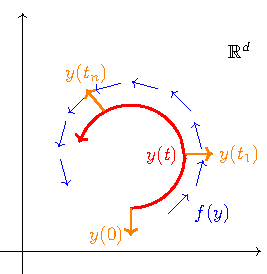
\includegraphics[width=4.47904368358914cm,height=4.59904237176964cm]{k1-1.pdf}}}
\end{remark*}

\begin{remark*}
  \tmtextbf{(Translationsinvarianz)}
  
  Bei einem autonomen System $y' = f (y)$ mit L{\"o}sung $y : I \rightarrow
  \mathbb{R}^d$ ist jede zeitversetzte Funktion ebenfalls eine L{\"o}sung des
  Systems. Konkret hei{\ss}t es:
  
  F{\"u}r $\Delta_t \in \mathbb{R}$, $\overline{I} \assign \{ t - \Delta_t |
  t \in I \nobracket \}$ ein verschobenes Zeitinvervall setze
  \[ \forall t \in \bar{I} : \text{\enspace} \bar{y} (t) \assign y (t +
     \Delta_t) . \]
  {\hspace{1.7em}}$\Rightarrow$ \ $\bar{y}' (t) = y' (t + \Delta_t) = f (y (t
  + \Delta_t)) = f (\bar{y} (t)) .$
  
  D.h. i.A. ist keine Eindeutigkeit der L{\"o}sungen von DGLn zu erwarten. 
\end{remark*}

Die Eigenschaft der Translationsinvarianz motiviert auch die Einf{\"u}hrung
der Anfangswertbedingung. Bevor dies tats{\"a}chlich geschieht, schauen wir
uns weitere Beispiele an:

\begin{example*}
  \tmtextbf{(Populationsmodelle)}
  
  Unter einer unbekannten {\underline{\tmtextit{Populationsgr{\"o}{\ss}e}}} $p
  (t)$ bzgl. Zeitparameter $t$ und Startzeit $t_0$ versetht man eine
  L{\"o}sung von
  \[ p (t_0) = p_0 \in \mathbb{R}_+ \enspace \wedge \text{\enspace} \forall t
     \in [t_0, \infty) : \text{ } p' (t) = r (t, p (t)) \cdot p (t) \]
  mit $r (t, p)$ der {\underline{\tmtextit{relativen {\"A}nderungsrate}}}.
  \begin{enumerateroman}
    \item Eine {\underline{\tmtextit{konstante Wachstumsrate}}} $r (t, p) =
    \alpha \in \mathbb{R}$ liefert ein exponentielles Wachstum mit L{\"o}sung
    \[ p (t) = p_0  \cdot \mathbf{e}^{\alpha (t - t_0)} . \]
    D.h. wir erhalten
    \[ \lim_{t \rightarrow \infty} p (t) = \left\{\begin{array}{l}
         \infty, \alpha > 0,\\
         p_0, \alpha = 0,\\
         0 \enspace, \alpha < 0.
       \end{array}\right. \]
    Graphisch sieht es dann aus wie
    
    \tmscriptoutput{graph}{Graph}{\
    
    \begin{tmcode}
    \tmverbatim{\%pdflatex}
    \end{tmcode}
    
    \begin{tmcode}
    \tmverbatim{\textbackslash textbackslash
    documentclass\textbackslash\{standalone\textbackslash\} \ \ }
    \end{tmcode}
    
    \begin{tmcode}
    \tmverbatim{\textbackslash textbackslash
    usepackage\textbackslash\{tikz\textbackslash\} \ \ }
    \end{tmcode}
    
    \begin{tmcode}
    \tmverbatim{\textbackslash textbackslash
    usepackage\textbackslash\{amssymb\textbackslash\} \ }
    \end{tmcode}
    
    \begin{tmcode}
    \tmverbatim{\textbackslash textbackslash
    usepackage\textbackslash\{amsmath\textbackslash\}}
    \end{tmcode}
    
    \begin{tmcode}
    \tmverbatim{\textbackslash textbackslash
    usepackage\textbackslash\{quiver\textbackslash\}}
    \end{tmcode}
    
    \begin{tmcode}
    \tmverbatim{\textbackslash textbackslash
    usepackage\textbackslash\{mathrsfs\textbackslash\}}
    \end{tmcode}
    
    \begin{tmcode}
    \tmverbatim{\textbackslash textbackslash
    begin\textbackslash\{document\textbackslash\}}
    \end{tmcode}
    
    \begin{tmcode}
    \tmverbatim{\textbackslash textbackslash
    begin\textbackslash\{tikzpicture\textbackslash\}}
    \end{tmcode}
    
    \begin{tmcode}
    \tmverbatim{\% drawing coordinate axis}
    \end{tmcode}
    
    \begin{tmcode}
    \tmverbatim{\textbackslash textbackslash
    draw[->](-0.3,0)--(3.2,0)node[left,below,font=\textbackslash textbackslash
    tiny]\textbackslash\{\$t\$\textbackslash\};}
    \end{tmcode}
    
    \begin{tmcode}
    \tmverbatim{\textbackslash textbackslash
    draw[->](0,-0.3)--(0,3.2)node[above,font=\textbackslash textbackslash
    tiny]\textbackslash\{\$p(t)\$\textbackslash\};}
    \end{tmcode}
    
    \begin{tmcode}
    \tmverbatim{\%noting points on axis}
    \end{tmcode}
    
    \begin{tmcode}
    \tmverbatim{\textbackslash textbackslash draw(0.4,0) node[below]
    \textbackslash\{\$t\_0\$\textbackslash\};}
    \end{tmcode}
    
    \begin{tmcode}
    \tmverbatim{\textbackslash textbackslash foreach \textbackslash
    textbackslash x in \textbackslash\{0.4\textbackslash\}
    \textbackslash\{\textbackslash textbackslash draw(\textbackslash
    textbackslash x,0)--(\textbackslash textbackslash x,0.1);\textbackslash\}}
    \end{tmcode}
    
    \begin{tmcode}
    \tmverbatim{\textbackslash textbackslash draw(0,0.8) node[left]
    \textbackslash\{\$p\_0\$\textbackslash\};}
    \end{tmcode}
    
    \begin{tmcode}
    \tmverbatim{\textbackslash textbackslash foreach \textbackslash
    textbackslash y in \textbackslash\{0.8\textbackslash\}
    \textbackslash\{\textbackslash textbackslash draw(0,\textbackslash
    textbackslash y)--(0.1,\textbackslash textbackslash y);\textbackslash\}}
    \end{tmcode}
    
    \begin{tmcode}
    \tmverbatim{\%drawing functions}
    \end{tmcode}
    
    \begin{tmcode}
    \tmverbatim{\textbackslash textbackslash draw[color=blue, smooth, line
    width = 1pt,domain=0.4:3]plot(\textbackslash textbackslash
    x,0.8)node[above]\textbackslash\{\$\textbackslash textbackslash
    alpha=0\$\textbackslash\};}
    \end{tmcode}
    
    \begin{tmcode}
    \tmverbatim{\textbackslash textbackslash draw[color=blue, line width =
    1pt, domain=0.4:3]plot (\textbackslash textbackslash x,
    \textbackslash\{0.8*exp(0.5*(\textbackslash textbackslash
    x-0.4))\textbackslash\})node[above]\textbackslash\{\$\textbackslash
    textbackslash alpha>0\$\textbackslash\};}
    \end{tmcode}
    
    \begin{tmcode}
    \tmverbatim{\textbackslash textbackslash draw[color=blue, line width =
    1pt, domain=0.4:3]plot (\textbackslash textbackslash x,
    \textbackslash\{0.8*exp(-1*(\textbackslash textbackslash
    x-0.4))\textbackslash\})node[above]\textbackslash\{\$\textbackslash
    textbackslash alpha<0\$\textbackslash\};}
    \end{tmcode}
    
    \begin{tmcode}
    \tmverbatim{\%\textbackslash textbackslash draw[color=red,
    thick,smooth,domain=-1:-0.02]plot(\textbackslash textbackslash x,0);}
    \end{tmcode}
    
    \begin{tmcode}
    \tmverbatim{\%\textbackslash textbackslash
    draw[color=red,smooth]circle(0.02);}
    \end{tmcode}
    
    \begin{tmcode}
    \tmverbatim{\textbackslash textbackslash
    end\textbackslash\{tikzpicture\textbackslash\}}
    \end{tmcode}
    
    \begin{tmcode}
    \tmverbatim{\textbackslash textbackslash
    end\textbackslash\{document\textbackslash\}}
    \end{tmcode}
    
    \begin{tmcode}
    \tmverbatim{\\
    }
    \end{tmcode}}{{\hspace{11em}}\raisebox{-0.00189410754979431\height}{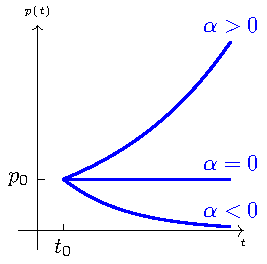
\includegraphics[width=4.47904368358914cm,height=4.43250688705234cm]{k1-2.pdf}}{\hspace{10em}}
    Sp{\"a}ter bezeichnen wir den Fall $\alpha > 0$
    {\underline{\tmtextit{instabil}}} und den Fall $\alpha \leq 0$
    {\underline{\tmtextit{stabil}}}. Im Allgemeinen ist konstante
    Wachstumsrate in biologischen Systemen eher unrealistisch.}
    
    \item Das Modell mit einem {\underline{\tmtextit{beschr{\"a}nkten}
    \tmtextit{Wachstums}\tmtextit{}}} ist eine Modifikation und dabei
    verwendet man den Ansatz
    \[ r (t, p) = \beta \cdot (\xi - p) \enspace \text{mit} \enspace \beta,
       \xi \in \mathbb{R_+} . \]
    Die Motivation des Ansatzes besteht darin, dass die Population mit der
    Zeit gegen einen Schwellwert $\xi$ konvergieren sollte. Um dies zu sehen,
    betrachenten wir die DGL unter diesem Ansatz:
    \[ p' = r \cdot p = \beta (\xi - p) \cdot p = \beta \xi p - \beta p^2 .
    \]
    Mit $\alpha \assign \beta \xi$ erhalten wir die sogenannte
    {\underline{\tmtextit{logistische DGL}}}
    \[ p' = \alpha p - \beta p^2 . \]
    Die L{\"o}sung der logistische DGL erweist sich als
    \begin{equation}
      p (t) = \xi \frac{p_0}{p_0 + (\xi - p_0) \mathbf{e}^{- \alpha (t - t
      0)}}
    \end{equation}
    und somit sieht man leicht, dass
    \[ \lim_{t \rightarrow \infty} p (t) = \xi \]
    gilt, bzw. graphisch erh{\"a}lt man
    
    \tmscriptoutput{graph}{Graph}{\
    
    \begin{tmcode}
    \tmverbatim{\%pdflatex}
    \end{tmcode}
    
    \begin{tmcode}
    \tmverbatim{\textbackslash textbackslash
    documentclass\textbackslash\{standalone\textbackslash\} \ \ }
    \end{tmcode}
    
    \begin{tmcode}
    \tmverbatim{\textbackslash textbackslash
    usepackage\textbackslash\{tikz\textbackslash\} \ \ }
    \end{tmcode}
    
    \begin{tmcode}
    \tmverbatim{\textbackslash textbackslash
    usepackage\textbackslash\{amssymb\textbackslash\} \ }
    \end{tmcode}
    
    \begin{tmcode}
    \tmverbatim{\textbackslash textbackslash
    usepackage\textbackslash\{amsmath\textbackslash\}}
    \end{tmcode}
    
    \begin{tmcode}
    \tmverbatim{\textbackslash textbackslash
    usepackage\textbackslash\{quiver\textbackslash\}}
    \end{tmcode}
    
    \begin{tmcode}
    \tmverbatim{\textbackslash textbackslash
    usepackage\textbackslash\{mathrsfs\textbackslash\}}
    \end{tmcode}
    
    \begin{tmcode}
    \tmverbatim{\textbackslash textbackslash
    begin\textbackslash\{document\textbackslash\}}
    \end{tmcode}
    
    \begin{tmcode}
    \tmverbatim{\textbackslash textbackslash
    begin\textbackslash\{tikzpicture\textbackslash\}}
    \end{tmcode}
    
    \begin{tmcode}
    \tmverbatim{\% drawing coordinate axis lines}
    \end{tmcode}
    
    \begin{tmcode}
    \tmverbatim{\textbackslash textbackslash
    draw[->](-0.3,0)--(3.2,0)node[left,below,font=\textbackslash textbackslash
    tiny]\textbackslash\{\$t\$\textbackslash\};}
    \end{tmcode}
    
    \begin{tmcode}
    \tmverbatim{\textbackslash textbackslash
    draw[->](0,-0.3)--(0,3.2)node[above,font=\textbackslash textbackslash
    tiny]\textbackslash\{\$p(t)\$ \textbackslash\};}
    \end{tmcode}
    
    \begin{tmcode}
    \tmverbatim{\%noting points on axis}
    \end{tmcode}
    
    \begin{tmcode}
    \tmverbatim{\textbackslash textbackslash draw(0.4,0) node[below]
    \textbackslash\{\$t\_0\$\textbackslash\};}
    \end{tmcode}
    
    \begin{tmcode}
    \tmverbatim{\textbackslash textbackslash foreach \textbackslash
    textbackslash x in \textbackslash\{0.4\textbackslash\}
    \textbackslash\{\textbackslash textbackslash draw(\textbackslash
    textbackslash x,0)--(\textbackslash textbackslash x,0.1);\textbackslash\}}
    \end{tmcode}
    
    \begin{tmcode}
    \tmverbatim{\textbackslash textbackslash draw(0,0.8) node[left]
    \textbackslash\{\$\textbackslash textbackslash xi\$\textbackslash\};}
    \end{tmcode}
    
    \begin{tmcode}
    \tmverbatim{\textbackslash textbackslash foreach \textbackslash
    textbackslash y in \textbackslash\{0.8\textbackslash\}
    \textbackslash\{\textbackslash textbackslash draw(0,\textbackslash
    textbackslash y)--(0.1,\textbackslash textbackslash y);\textbackslash\}}
    \end{tmcode}
    
    \begin{tmcode}
    \tmverbatim{\%drawing functions}
    \end{tmcode}
    
    \begin{tmcode}
    \tmverbatim{\textbackslash textbackslash draw[color=blue, smooth, line
    width = 1pt,domain=0.4:3.2]plot(\textbackslash textbackslash
    x,0.8)node[above]\textbackslash\{ \textbackslash\};}
    \end{tmcode}
    
    \begin{tmcode}
    \tmverbatim{\textbackslash textbackslash draw[color=blue, line width =
    1pt, domain=0.4:3.2]plot (\textbackslash textbackslash x,
    \textbackslash\{0.8*2.4/(2.4 + (0.8-2.4)*exp(0.8*(0.4-\textbackslash
    textbackslash x)) ) \ \textbackslash\})node[right]\textbackslash\{
    \textbackslash\};}
    \end{tmcode}
    
    \begin{tmcode}
    \tmverbatim{\textbackslash textbackslash draw[color=blue, line width =
    1pt, domain=0.4:3.2]plot (\textbackslash textbackslash x,
    \textbackslash\{0.8*0.2/(0.2 + (0.8-0.2)*exp(1.3*(0.4-\textbackslash
    textbackslash x)) ) \ \textbackslash\})node[below]\textbackslash\{ \
    \textbackslash\};}
    \end{tmcode}
    
    \begin{tmcode}
    \tmverbatim{\textbackslash textbackslash draw[color=blue](1,2.7)
    node[below] \textbackslash\{\$p\_0>\textbackslash textbackslash
    xi\$\textbackslash\};}
    \end{tmcode}
    
    \begin{tmcode}
    \tmverbatim{\textbackslash textbackslash draw[color=blue](0.6,1.3)
    node[below] \textbackslash\{\$p\_0=\textbackslash textbackslash
    xi\$\textbackslash\};}
    \end{tmcode}
    
    \begin{tmcode}
    \tmverbatim{\textbackslash textbackslash draw[color=blue](2,0.6)
    node[below] \textbackslash\{\$p\_0<\textbackslash textbackslash
    xi\$\textbackslash\};}
    \end{tmcode}
    
    \begin{tmcode}
    \tmverbatim{\textbackslash textbackslash
    end\textbackslash\{tikzpicture\textbackslash\}}
    \end{tmcode}
    
    \begin{tmcode}
    \tmverbatim{\textbackslash textbackslash
    end\textbackslash\{document\textbackslash\}}
    \end{tmcode}}{{\hspace{11em}}\raisebox{-0.00176482956641033\height}{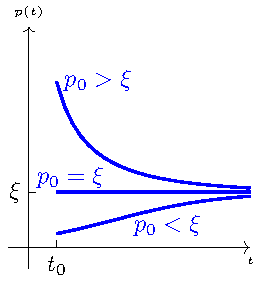
\includegraphics[width=4.47904368358914cm,height=4.75719860947134cm]{k1-3.pdf}}{\hspace{12em}}
    Man kann auch leicht ausrechnen, dass $\tmop{sgn} (p') = \tmop{sgn} (\xi -
    p_0)$ konstant ist, und das zeigt nochmal die monotone Konvergenz von $p$
    gegen $\xi .$}
  \end{enumerateroman}
\end{example*}

Obige beiden Modelle beschreiben biologische Systeme mit einer Spezies, aber
typischerweise sind biologische Systeme komplizierter. Das folgende Modell
betrachtet die Populationen zweier Spezies mit einem gewissen Zusammenhang:

\begin{example*}
  \tmtextbf{(R{\"a}uber-Beute-Modelle)}
  
  Sei $x (t)$ die Populationsgr{\"o}{\ss}e der Beutespezies und $y (t)$ die
  Populationsgr{\"o}{\ss}e der R{\"a}uberspezies.
  
  Intuitive w{\"u}rde man schon erwarten, dass die relativen
  {\"A}nderungsraten beider Spezies durch jeweils die Andere beeinflusst
  werden.
  
  Diese Situation kann man mit den
  {\underline{\tmtextit{Lotka-Volterra-Gleichungen}}} bzgl. Paramter $\alpha,
  \beta, \gamma, \delta > 0$ modellieren, also
  \[ \left\{\begin{array}{l}
       x' = (\alpha - \beta y) x,\\
       y' = (- \gamma + \delta x) y,
     \end{array}\right. \]
  mit den folgenden Interpretationen:
  
  {\hspace{3em}}$\alpha \hspace{0.47em} :$\quad Wachstumsrate von $x$ ohne
  R{\"a}uber $y$,
  
  {\hspace{3em}}$\beta y :$\quad Sterberate von $x$ durch R{\"a}uber $y$,
  
  {\hspace{3em}}$\gamma \hspace{0.37em} :$\quad Sterberate von $y$ ohne Beute
  $y$,
  
  {\hspace{3em}}$\delta x :$\quad Wachstumsrate von $y$ bei Vorhandensein von
  Beute $x$.
  
  F{\"u}r solche Systeme sind ihre station{\"a}re Punkte interessant, d.h.
  Punkte, wo die Ableitungen verschwinden. Dazu kann man sich leicht
  {\"u}berlegen:
  \[ \left(\begin{array}{c}
       x'\\
       y'
     \end{array}\right) = \left(\begin{array}{c}
       0\\
       0
     \end{array}\right) \quad \Leftrightarrow \text{\quad}
     \left(\begin{array}{c}
       x (t)\\
       y (t)
     \end{array}\right) \equiv \left(\begin{array}{c}
       0\\
       0
     \end{array}\right) \infixor \left(\begin{array}{c}
       x (t)\\
       y (t)
     \end{array}\right) = \left(\begin{array}{c}
       \gamma / \delta\\
       \alpha / \beta
     \end{array}\right) . \]
  
  
  Die m{\"o}glichen L{\"o}sungskurven kann man im Phasenraum visualisieren:
  
  \tmscriptoutput{graph}{Graph}{\
  
  \begin{tmcode}
  \tmverbatim{\%pdflatex}
  \end{tmcode}
  
  \begin{tmcode}
  \tmverbatim{\textbackslash textbackslash
  documentclass\textbackslash\{standalone\textbackslash\} \ \ }
  \end{tmcode}
  
  \begin{tmcode}
  \tmverbatim{\textbackslash textbackslash
  usepackage\textbackslash\{pgf\textbackslash\}}
  \end{tmcode}
  
  \begin{tmcode}
  \tmverbatim{\textbackslash textbackslash
  begin\textbackslash\{document\textbackslash\}}
  \end{tmcode}
  
  \begin{tmcode}
  \tmverbatim{\textbackslash textbackslash
  input\textbackslash\{/Users/Simba/Downloads/RBM1.pgf\textbackslash\}}
  \end{tmcode}
  
  \begin{tmcode}
  \tmverbatim{\textbackslash textbackslash
  end\textbackslash\{document\textbackslash\}}
  \end{tmcode}}{{\hspace{6em}}\raisebox{-0.0012163080300086\height}{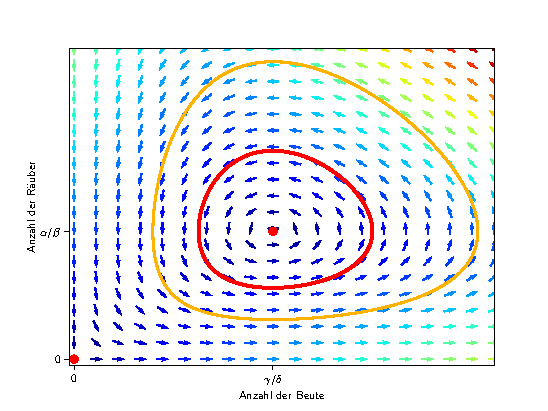
\includegraphics[width=9.20902203856749cm,height=6.90256460711006cm]{k1-4.pdf}}}
  
  Im Bild werden die Kurven mit negativen $x$ oder $y$ Werten nicht
  gezeichnet. Solche Kurven sind zwar mathematisch m{\"o}glich, aber wenig
  realistisch.
  
  Die Kurven sind geschlossen, denn sie sind H{\"o}henlinien von der Funktion
  \[ J : \mathbb{(R^+)^2 \rightarrow R}, \text{ } (x, y) \mapsto \gamma \ln
     (x) - \delta x + \alpha \ln (y) - \beta y. \]
  {\hspace{1.7em}}Genauer gesagt kann man zeigen, dass f{\"u}r jede L{\"o}sung
  $\left(\begin{array}{c}
    x (t)\\
    y (t)
  \end{array}\right)$ mit $t \in \mathbb{R}$ gilt
  \[ \frac{\upright{d}}{\upright{d} t} J (x (t), y (t)) = 0. \]
  {\hspace{1.7em}}Das bedeutet: Eine L{\"o}sung ist periodisch, wenn ein Punkt
  zum zweiten Mal erreicht wird, also:
  \[ \left(\begin{array}{c}
       x (\tau)\\
       y (\tau)
     \end{array}\right) = \left(\begin{array}{c}
       x (0)\\
       y (0)
     \end{array}\right) \quad \Rightarrow \text{\quad} \forall t \in
     \mathbb{R} \forall k \in \mathbb{Z} : \left(\begin{array}{c}
       x (t + k \tau)\\
       y (t + k \tau)
     \end{array}\right) = \left(\begin{array}{c}
       x (t)\\
       y (t)
     \end{array}\right) . \]
\end{example*}

Wir sehen: Ohne ,,Startpunkt`` ist keine eindeutige L{\"o}sung zu erwarten.

F{\"u}r den Rest des Kapitels betrachten wir nur noch Anfangswertprobleme:

\begin{definition}
  \tmtextbf{(AWP)}
  
  \tmtextit{Sei $d \in \mathbb{N}$, $D \subseteq \mathbb{R}^{d + 1}$}
  \tmtextit{ein Gebiet, $(t_0, y_0) \in D$ und $f : D \rightarrow
  \mathbb{R}^d$ stetig}.
  
  \tmtextit{Gesucht ist ein Intervall $I \subseteq \mathbb{R}$ mit $t_0 \in
  I$ und ein $y \in C^1 (I, \mathbb{R}^d)$, so dass}
  \begin{equation}
    y (t_0) = y_0 \quad \wedge \text{\quad} \forall t \in I : \text{ } y' (t)
    = f (t, y)
  \end{equation}
  \tmtextit{und man nennt $y$ die L{\"o}sung vom}
  {\underline{\tmtextit{Anfangswertproblem}}} (1.6). 
\end{definition}

Beachte: Der Fall $I = \mathbb{R}$ ist auch m{\"o}glich, falls es $D$ passt.

Der folgende Satz besagt, dass man ein Anfangswertproblem {\"a}quivalent
umformen kann:

\begin{theorem}
  \tmtextbf{(Volterra'sche Integralgleichung)}
  
  \tmtextit{Wir definieren die {\underline{Volterra'sche Integralgleichung
  (VI)}} als}
  \begin{equation}
    y (t) = y_0 + \int_{t_0}^t f (s, y (s)) \textrm{\upright{d}} s
  \end{equation}
  \tmtextit{und stellen fest, dass die folgende zwei Bedingungen
  {\"a}quivalent sind: }\tmtextit{}
  \begin{enumerateroman}
    \item \tmtextit{Eine L{\"o}sung $y \in C^1 (I, \mathbb{R}^d)$ des AWP
    (1.6) erf{\"u}llt (1.7) f{\"u}r alle $t \in I$;}
    
    \item \tmtextit{Eine Funktion $y \in C (I, \mathbb{R}^d)$, welche (1.7)
    f{\"u}r alle $t \in I$ erf{\"u}llt, ist eine L{\"o}sung des AWP (1.6),
    insbesondere ist $y$ stetig differenzierbar.}
  \end{enumerateroman}
\end{theorem}

\begin{proof}
  ,,i. $\Rightarrow$ ii.``
  
  Sei $y : I \rightarrow \mathbb{R}^d$ eine L{\"o}sung des AWPs.
  
  Die Fundamentalsatz der Differenzial-\&Integralrechnung liefert dann
  \[ \forall t \in I : \text{\quad} y (t) = y (t_0) + \int_{t_0}^t y' (s)
     \upright{d} s = y (t_0) + \int_{t_0}^t f (s, y (s)) \upright{d} s. \]
  {\hspace{5em}},,ii. $\Rightarrow$ i.``
  
  Sei $y : I \rightarrow \mathbb{R}^d$ stetig mit $t_0 \in I$ und $y$
  erf{\"u}lle VI (1.7).
  
  $y$ erf{\"u}llt die Anfangswertbedingung, denn mit $t = t_0$ gilt
  \[ y (t_0) = y_0 + \int_{t_0}^{t_0} f (s, y (s)) \upright{d} s = y_0 . \]
  {\hspace{1.7em}}Da $f (s, y (s))$ stetig bzgl. $s$ ist, ist $y (t) =
  \int_{t_0}^t f (s, y (s)) \upright{d} s$ als Integral stetiger Funktion
  differenzierbar, und somit
  \[ y' (t) = \frac{\upright{d}}{\upright{d} t} \left( y (t_0) + \int_{t_0}^t
     f (s, y (s)) \upright{d} s \right) = 0 + f (t, y (t)) \]
  also ist $y$ eine L{\"o}sung vom AWP (1.6). 
\end{proof}

Besitzt ein AWP (1.6) immer eine L{\"o}sung? Ja, da $f$ als stetig
vorausgesetzt ist:

\begin{theorem}
  \tmtextbf{(Existenzsatz von Peano)}
  
  \tmtextit{Jedes AWP (1.6) mit stetigem $f : D \rightarrow \mathbb{R}^d$
  besitzt mindestens eine lokale L{\"o}sung $y : I_0 \rightarrow
  \mathbb{R}^d$, welche sich auf den Rand von $D$ fortsetzen l{\"a}sst. }
\end{theorem}

Wir verzichten hier auf den Beweis dieses Satzes.

\begin{remark*}
  \tmtextbf{(zur Fortsetzbarkeit einer L{\"o}sung)}
  
  Sei $I_0 = (t_1, t_2)$. Dann ist die Fortsetzung eventuell sowohl f{\"u}r $t
  > t_2$ als auch f{\"u}r $t < t_1$ m{\"o}glich, bis Rand $\partial D$
  erreicht wird.
  
  Zu einer L{\"o}sung $y : I_0 \rightarrow \mathbb{R}^d$ existiert also ein
  maximales Existenzintervall $I_{\max}$, welches wir im folgenden oft einfach
  als $I$ bezeichnen.
  
  Dieses maximale Existenzintervall $I_{\max} = I$ kann aber ,,alle
  m{\"o}glichen Formen`` haben: vielleicht beschr{\"a}nkt, oder vielleicht
  unbeschr{\"a}nkt, oder vielleicht abgeschlossen, halb-offen{\textdots}Wir
  schauen uns einige Beispiele an:
  \begin{enumerateroman}
    \item L{\"o}sung nur auf Halbachsen, d.h. f{\"u}r endliche Zeit:
    \[ y' = y^2 \enspace \wedge \text{\enspace} D = \mathbb{R^2} . \]
    F{\"u}r $a \in \mathbb{R}$ (von der Anfangswertbedingung abh{\"a}ngig) ist
    die Funktion
    \[ y (t) = \frac{1}{a - t} \]
    eine L{\"o}sung dieser DGL, denn
    \[ y' (t) = - \frac{1}{(a - t)^2} (- 1) = \frac{1}{(a - t)^2} = y (t)^2 .
    \]
    \tmscriptoutput{graph}{Graph}{\
    
    \begin{tmcode}
    \tmverbatim{\%pdflatex}
    \end{tmcode}
    
    \begin{tmcode}
    \tmverbatim{\textbackslash textbackslash
    documentclass\textbackslash\{standalone\textbackslash\} \ \ }
    \end{tmcode}
    
    \begin{tmcode}
    \tmverbatim{\textbackslash textbackslash
    usepackage\textbackslash\{tikz\textbackslash\} \ \ }
    \end{tmcode}
    
    \begin{tmcode}
    \tmverbatim{\textbackslash textbackslash
    usepackage\textbackslash\{amssymb\textbackslash\} \ }
    \end{tmcode}
    
    \begin{tmcode}
    \tmverbatim{\textbackslash textbackslash
    usepackage\textbackslash\{amsmath\textbackslash\}}
    \end{tmcode}
    
    \begin{tmcode}
    \tmverbatim{\textbackslash textbackslash
    usepackage\textbackslash\{quiver\textbackslash\}}
    \end{tmcode}
    
    \begin{tmcode}
    \tmverbatim{\textbackslash textbackslash
    usepackage\textbackslash\{mathrsfs\textbackslash\}}
    \end{tmcode}
    
    \begin{tmcode}
    \tmverbatim{\textbackslash textbackslash
    begin\textbackslash\{document\textbackslash\}}
    \end{tmcode}
    
    \begin{tmcode}
    \tmverbatim{\textbackslash textbackslash
    begin\textbackslash\{tikzpicture\textbackslash\}}
    \end{tmcode}
    
    \begin{tmcode}
    \tmverbatim{\% drawing coordinate axis lines}
    \end{tmcode}
    
    \begin{tmcode}
    \tmverbatim{\textbackslash textbackslash
    draw[->](-3,0)--(4,0)node[left,below,font=\textbackslash textbackslash
    tiny]\textbackslash\{\$t\$\textbackslash\};}
    \end{tmcode}
    
    \begin{tmcode}
    \tmverbatim{\textbackslash textbackslash
    draw[->](0,-3)--(0,4)node[above,font=\textbackslash textbackslash
    tiny]\textbackslash\{\textbackslash\};}
    \end{tmcode}
    
    \begin{tmcode}
    \tmverbatim{\textbackslash textbackslash draw[densely
    dotted](1,-3)--(1,4)node[above,font=\textbackslash textbackslash
    tiny]\textbackslash\{\textbackslash\};}
    \end{tmcode}
    
    \begin{tmcode}
    \tmverbatim{\%noting points on axis}
    \end{tmcode}
    
    \begin{tmcode}
    \tmverbatim{\textbackslash textbackslash draw(1,0) node[below]
    \textbackslash\{\$a\$\textbackslash\};}
    \end{tmcode}
    
    \begin{tmcode}
    \tmverbatim{\textbackslash textbackslash foreach \textbackslash
    textbackslash x in \textbackslash\{1\textbackslash\}
    \textbackslash\{\textbackslash textbackslash draw(\textbackslash
    textbackslash x,0)--(\textbackslash textbackslash x,0.1);\textbackslash\}}
    \end{tmcode}
    
    \begin{tmcode}
    \tmverbatim{\%\textbackslash textbackslash draw(0,0.8) node[left]
    \textbackslash\{\$p\_0\$\textbackslash\};}
    \end{tmcode}
    
    \begin{tmcode}
    \tmverbatim{\%\textbackslash textbackslash foreach \textbackslash
    textbackslash y in \textbackslash\{0.8\textbackslash\}
    \textbackslash\{\textbackslash textbackslash draw(0,\textbackslash
    textbackslash y)--(0.1,\textbackslash textbackslash y);\textbackslash\}}
    \end{tmcode}
    
    \begin{tmcode}
    \tmverbatim{\\
    }
    \end{tmcode}
    
    \begin{tmcode}
    \tmverbatim{\%drawing functions}
    \end{tmcode}
    
    \begin{tmcode}
    \tmverbatim{\textbackslash textbackslash draw[color=blue, line width =
    1pt, domain=-3:0.75]plot (\textbackslash textbackslash x, \textbackslash\{
    1/(1-\textbackslash textbackslash x)
    \textbackslash\})node[right]\textbackslash\{ \textbackslash\};}
    \end{tmcode}
    
    \begin{tmcode}
    \tmverbatim{\textbackslash textbackslash draw[color=blue, line width =
    1pt, domain=1.35:4]plot (\textbackslash textbackslash x, \textbackslash\{
    1/(1-\textbackslash textbackslash x)
    \textbackslash\})node[below]\textbackslash\{\$y(t)\$ \textbackslash\};}
    \end{tmcode}
    
    \begin{tmcode}
    \tmverbatim{\%\textbackslash textbackslash draw[color=blue, line width =
    1pt, domain=0.4:3]plot (\textbackslash textbackslash x,
    \textbackslash\{0.8*exp(-1*(\textbackslash textbackslash
    x-0.4))\textbackslash\})node[above]\textbackslash\{\$\textbackslash
    textbackslash alpha<0\$\textbackslash\};}
    \end{tmcode}
    
    \begin{tmcode}
    \tmverbatim{\textbackslash textbackslash
    end\textbackslash\{tikzpicture\textbackslash\}}
    \end{tmcode}
    
    \begin{tmcode}
    \tmverbatim{\textbackslash textbackslash
    end\textbackslash\{document\textbackslash\}}
    \end{tmcode}}{{\hspace{12em}}\raisebox{-0.00192366939937932\height}{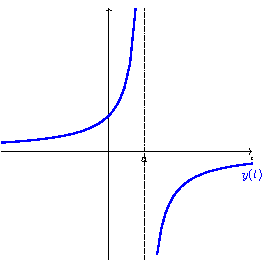
\includegraphics[width=4.47904368358914cm,height=4.36439065984521cm]{k1-5.pdf}}{\hspace{11em}}
    Offensichtlich ist $y$ nur auf $(- \infty, a)$ oder $(a, \infty)$ sinnvoll
    definiert, und welches Intervall der Beiden als $I_{\max}$ genommen wird,
    h{\"a}ngt davon ab, in welchem Intervall $t_0$ liegt.}
    
    \item L{\"o}sung nur auf endlichem Intervall:
    \[ y' = 1 + y^2 . \]
    F{\"u}r $c \in \mathbb{R}$ (von der Anfangswertbedingung abh{\"a}ngig) ist
    die Funktion
    \[ y (t) = \tan (t - c) \]
    eine L{\"o}sung der DGL und wegen der Polstellen von $\tan$ kann
    $I_{\max}$ h{\"o}chstens $\left( c - \frac{\pi}{2}, c + \frac{\pi}{2}
    \right)$ sein.
    
    \tmscriptoutput{graph}{Graph}{\
    
    \begin{tmcode}
    \tmverbatim{\%pdflatex}
    \end{tmcode}
    
    \begin{tmcode}
    \tmverbatim{\textbackslash textbackslash
    documentclass\textbackslash\{standalone\textbackslash\} \ \ }
    \end{tmcode}
    
    \begin{tmcode}
    \tmverbatim{\textbackslash textbackslash
    usepackage\textbackslash\{tikz\textbackslash\} \ \ }
    \end{tmcode}
    
    \begin{tmcode}
    \tmverbatim{\textbackslash textbackslash
    usepackage\textbackslash\{amssymb\textbackslash\} \ }
    \end{tmcode}
    
    \begin{tmcode}
    \tmverbatim{\textbackslash textbackslash
    usepackage\textbackslash\{amsmath\textbackslash\}}
    \end{tmcode}
    
    \begin{tmcode}
    \tmverbatim{\textbackslash textbackslash
    usepackage\textbackslash\{quiver\textbackslash\}}
    \end{tmcode}
    
    \begin{tmcode}
    \tmverbatim{\textbackslash textbackslash
    usepackage\textbackslash\{mathrsfs\textbackslash\}}
    \end{tmcode}
    
    \begin{tmcode}
    \tmverbatim{\textbackslash textbackslash
    begin\textbackslash\{document\textbackslash\}}
    \end{tmcode}
    
    \begin{tmcode}
    \tmverbatim{\textbackslash textbackslash
    begin\textbackslash\{tikzpicture\textbackslash\}}
    \end{tmcode}
    
    \begin{tmcode}
    \tmverbatim{\% drawing coordinate axis lines}
    \end{tmcode}
    
    \begin{tmcode}
    \tmverbatim{\textbackslash textbackslash
    draw[->](-3,0)--(3,0)node[left,below,font=\textbackslash textbackslash
    tiny]\textbackslash\{\$t\$\textbackslash\};}
    \end{tmcode}
    
    \begin{tmcode}
    \tmverbatim{\textbackslash textbackslash
    draw[->](-0.5,-3)--(-0.5,3)node[above,font=\textbackslash textbackslash
    tiny]\textbackslash\{\textbackslash\};}
    \end{tmcode}
    
    \begin{tmcode}
    \tmverbatim{\textbackslash textbackslash draw[densely
    dotted](1.5,-3)--(1.5,3)node[above,font=\textbackslash textbackslash
    tiny]\textbackslash\{\textbackslash\};}
    \end{tmcode}
    
    \begin{tmcode}
    \tmverbatim{\textbackslash textbackslash draw[densely
    dotted](-1.5,-3)--(-1.5,3)node[above,font=\textbackslash textbackslash
    tiny]\textbackslash\{\textbackslash\};}
    \end{tmcode}
    
    \begin{tmcode}
    \tmverbatim{\%noting points on axis}
    \end{tmcode}
    
    \begin{tmcode}
    \tmverbatim{\textbackslash textbackslash draw(0,0) node[below]
    \textbackslash\{\$c\$\textbackslash\};}
    \end{tmcode}
    
    \begin{tmcode}
    \tmverbatim{\textbackslash textbackslash foreach \textbackslash
    textbackslash x in \textbackslash\{0\textbackslash\}
    \textbackslash\{\textbackslash textbackslash draw(\textbackslash
    textbackslash x,0)--(\textbackslash textbackslash x,0.1);\textbackslash\}}
    \end{tmcode}
    
    \begin{tmcode}
    \tmverbatim{\textbackslash textbackslash draw(1.5,0) node[below]
    \textbackslash\{\$c+\textbackslash textbackslash
    frac\textbackslash\{\textbackslash textbackslash
    pi\textbackslash\}\textbackslash\{2\textbackslash\}\$\textbackslash\};}
    \end{tmcode}
    
    \begin{tmcode}
    \tmverbatim{\textbackslash textbackslash foreach \textbackslash
    textbackslash x in \textbackslash\{1.5\textbackslash\}
    \textbackslash\{\textbackslash textbackslash draw(\textbackslash
    textbackslash x,0)--(\textbackslash textbackslash x,0.1);\textbackslash\}}
    \end{tmcode}
    
    \begin{tmcode}
    \tmverbatim{\textbackslash textbackslash draw(-1.5,0) node[below]
    \textbackslash\{\$c-\textbackslash textbackslash
    frac\textbackslash\{\textbackslash textbackslash
    pi\textbackslash\}\textbackslash\{2\textbackslash\}\$\textbackslash\};}
    \end{tmcode}
    
    \begin{tmcode}
    \tmverbatim{\textbackslash textbackslash foreach \textbackslash
    textbackslash x in \textbackslash\{-1.5\textbackslash\}
    \textbackslash\{\textbackslash textbackslash draw(\textbackslash
    textbackslash x,0)--(\textbackslash textbackslash x,0.1);\textbackslash\}}
    \end{tmcode}
    
    \begin{tmcode}
    \tmverbatim{\\
    }
    \end{tmcode}
    
    \begin{tmcode}
    \tmverbatim{\%\textbackslash textbackslash draw(0,0.8) node[left]
    \textbackslash\{\$p\_0\$\textbackslash\};}
    \end{tmcode}
    
    \begin{tmcode}
    \tmverbatim{\%\textbackslash textbackslash foreach \textbackslash
    textbackslash y in \textbackslash\{0.8\textbackslash\}
    \textbackslash\{\textbackslash textbackslash draw(0,\textbackslash
    textbackslash y)--(0.1,\textbackslash textbackslash y);\textbackslash\}}
    \end{tmcode}
    
    \begin{tmcode}
    \tmverbatim{\\
    }
    \end{tmcode}
    
    \begin{tmcode}
    \tmverbatim{\%drawing functions}
    \end{tmcode}
    
    \begin{tmcode}
    \tmverbatim{\textbackslash textbackslash draw[color=blue, line width =
    1pt, domain=-1.24:1.24]plot (\textbackslash textbackslash x,
    \textbackslash\{ tan(\textbackslash textbackslash x r)
    \textbackslash\})node[left]\textbackslash\{\$y(t)\$ \textbackslash\};}
    \end{tmcode}
    
    \begin{tmcode}
    \tmverbatim{\%\textbackslash textbackslash draw[color=blue, line width =
    1pt, domain=1.35:4]plot (\textbackslash textbackslash x, \textbackslash\{
    1/(1-\textbackslash textbackslash x)
    \textbackslash\})node[below]\textbackslash\{\$y(t)\$ \textbackslash\};}
    \end{tmcode}
    
    \begin{tmcode}
    \tmverbatim{\%\textbackslash textbackslash draw[color=blue, line width =
    1pt, domain=0.4:3]plot (\textbackslash textbackslash x,
    \textbackslash\{0.8*exp(-1*(\textbackslash textbackslash
    x-0.4))\textbackslash\})node[above]\textbackslash\{\$\textbackslash
    textbackslash alpha<0\$\textbackslash\};}
    \end{tmcode}
    
    \begin{tmcode}
    \tmverbatim{\textbackslash textbackslash
    end\textbackslash\{tikzpicture\textbackslash\}}
    \end{tmcode}
    
    \begin{tmcode}
    \tmverbatim{\textbackslash textbackslash
    end\textbackslash\{document\textbackslash\}}
    \end{tmcode}}{{\hspace{10em}}\raisebox{-0.00185676777347433\height}{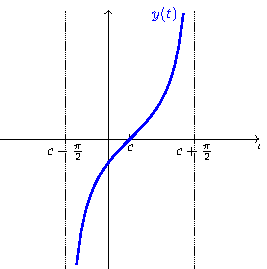
\includegraphics[width=4.47904368358914cm,height=4.52164502164502cm]{k1-6.pdf}}}
  \end{enumerateroman}
\end{remark*}

Satz von Peano besagt, jedes AWP mit stetigem $f$ besitzt eine L{\"o}sung,
aber diese muss nicht eindeutig sein:

\begin{example*}
  \tmtextbf{(Mehrdeutigkeit von L{\"o}sung eines AWPs)}
  
  F{\"u}r $d = 1$, $D = \mathbb{R \times \mathbb{R^+}}$ betrachte
  \[ y' = \sqrt{| y (t) |} \quad \wedge \text{\quad} y_0 \assign y (0) = 0.
  \]
  {\hspace{1.7em}}Das AWP besitzt zumindest zwei L{\"o}sungen $y (t) \equiv 0$
  und $y (t) = \frac{1}{4} t^2$.
\end{example*}

Also, f{\"u}r die (Existenz \&) Eindeutigkeit einer L{\"o}sung beim AWP sind
st{\"a}rkere Bedingungen erforderlich:

\begin{theorem}
  \tmtextbf{(Existenz \& Eindeutigkeit f{\"u}r AWP, Picard-Lindel{\"o}f)}
  
  \tmtextit{Sei ein AWP (1.6) gegeben, also insbesondere ist }$f$ stetig.
  
  \tmtextit{Sei au{\ss}erdem {\underline{$f$ Lipschitz-stetig bzgl. 2.
  Argument}}, d.h.}
  \[ \exists L \in \mathbb{R}_+ \hspace{0.3em} \forall (t, y), \left( t,
     \overline{y} \right) \in D : \text{ } \parallel f (t, y) - f \left( t,
     \overline{y} \right) \parallel \leq \text{ } L \parallel y - \overline{y}
     \parallel . \]
  {\hspace{1.7em}}\tmtextit{Dann existiert eine L{\"o}sung $y : I_0
  \rightarrow \mathbb{R}^d$, welche sich auf maximales Existenzintervall
  $I_{\max}$ fortsetzen l{\"a}sst und eindeutig ist.} 
\end{theorem}

\begin{remark*}
  {\tmdummy}
  
  \begin{itemizedot}
    \item Im Fall von \tmtextit{{\underline{steitgem, st{\"u}ckweise
    differenzierbarem $f$}}} gibt es eine Charakterisierung f{\"u}r die
    Lipschitz-Stetigkeit:
    \[ f \text{Lipschitz-stetig bzgl.} y \hspace{0.8em} \Leftrightarrow
       \text{{\hspace{0.8em}}} \frac{\partial}{\partial y} f
       \text{beschr{\"a}nkt durch Lipschitz-Konstante} L. \]
    Dies liefert dann auch einen einfachen und in der Praxis umsetzbaren Test.
    
    \item Die Funktion $f (t, y) = \sqrt{| y |}$ aus Beispiel zu
    Mehrdeutigkeit ist \tmtextit{{\underline{nicht}}} Lipschitz-stetig auf
    $D$, denn die partielle Ableitung
    \[ \frac{\partial}{\partial y} \sqrt{| y |} = \frac{1}{2 \sqrt{| y |}}
       \tmop{sgn} (y) \]
    ist unbeschr{\"a}nkt f{\"u}r $y \rightarrow 0$. Somit ist dabei der Satz
    1.5 nicht anwendbar.
  \end{itemizedot}
\end{remark*}

\begin{proof}
  (von 1.5)
  
  Existenz von L{\"o}sung $y : I \rightarrow \mathbb{R}^d$ f{\"u}r $I$ mit
  $I_0 \subseteq I \subseteq I_{\max}$ folgt aus Peano \& Fortsetzbarkeit.
  
  Interessant ist die Eindeutigkeit:
  
  OBdA sei $I$ kompakt (sonst folgt Eindeutigkeit durch Aussch{\"o}pfen von
  $I$ mit kompakten Intervallen).
  
  Wir zeigen die {\underline{\tmtextit{Eindeutigkeit mit dem Banach'schen
  Fixpunktsatzes (BFS)}}}.
  \begin{enumeratealpha}
    \item Definiere auf $C (I, \mathbb{R}^d)$ \ eine neue ,,gewichtete`` Norm
    $\parallel \bullet \parallel_{\alpha, t_0}$ zu Parametern $\alpha > 0$,
    $t_0 \in I$:
    \[ \forall u \in C (I, \mathbb{R}^d) : \text{\quad}  \parallel \text{ } u
       \parallel_{\alpha, t_0} \assign \sup_{t \in I} \left| u (t)
       {{\mathbf{e}^{- \alpha (t - t_0)}} }  \right| . \]
    {\hspace{1.7em}}Man kann nachrechnen, dass dies tats{\"a}chlich eine Norm
    ist (Beweis {\"a}hnlich zu $\parallel \bullet \parallel_{\infty}$) und
    Cauchy-Folgen in $C (I, \mathbb{R}^d)$ bzgl. dieser Norm
    gleichm{\"a}{\ss}ig konvergieren, d.h. $C (I, \mathbb{R}^d)$ ist
    vollst{\"a}ndig.
    
    \item W{\"a}hle von $C (I, \mathbb{R}^d)$ eine Teilmenge
    (Definitionsbereich von Kontraktion)
    \[ M \assign \{ \nobracket y \in C (I, \mathbb{R}^d) | y (t_0) = y_0 \} .
    \]
    $M$ ist abgeschlossen bzgl. $\parallel \bullet \parallel_{\alpha, t_0}$,
    denn f{\"u}r $(u_k)_{k \in \mathbb{N}} \in \tmop{CF} (C (I, \mathbb{R}^d),
    \parallel \bullet \parallel_{\alpha, t_0})$ existiert ein $u \in C (I,
    \mathbb{R}^d)$ so dass $u_k \xrightarrow{\text{glm.}} u$, da $(C (I,
    \mathbb{R}^d), \parallel \bullet \parallel_{\alpha, t_0})$ vollst{\"a}ndig
    ist. Damit gilt $u (t_0) = \lim_{k \rightarrow \infty} u_k (t_0) = y_0$,
    also ist $u \in M$.
    
    \item Definiere die Abbildung $\Phi$ durch die Volterra'sche
    Integralgleichung (VI), d.h. f{\"u}r $u \in M$ setze \
    \[ \Phi (u) (t) \assign y_0 + \int_{t_0}^t f (s, u (s)) \upright{d} s, t
       \in I. \]
    Es gilt $\Phi (u) \in C (I, \mathbb{R}^d)$, denn mit Stetigkeit von $u$
    und $f$ ist das Integrand stetig, und somit $\Phi (u)$ als Integral
    stetiger Funktion stetig.
    
    Zudem ist $\Phi (u) (t_0) = y_0$, also ist $\Phi : M \rightarrow M$ eine
    Selbstabbildung.
    
    Es bleibt noch die Kontraktionseigenschaft zu zeigen.
    
    \item F{\"u}hre eine punktweise Absch{\"a}tzung von $\Phi (-) (t)$ durch,
    also f{\"u}r $u, \bar{u} \in M$ und $t \geq t_0$ gilt:
    \begin{eqnarray*}
      \left| \Phi (u) (t) - \Phi \left( \overline{u} \right) (t) \right| & = &
      \left| \int_{t_0}^t f (s, u (s)) - f (s, \bar{u} (s)) \upright{d} s
      \right|\\
      & \leq & \int_{t_0}^t | f (s, u (s)) - f (s, \bar{u} (s)) | \upright{d}
      s\\
      & \leq & L \int_{t_0}^t | u (s) - \bar{u} (s) | \upright{d} s\\
      & = & L \int_{t_0}^t | u (s) - \bar{u} (s) | \mathbf{e}^{- \alpha | s -
      t_0 |} \mathbf{e}^{\alpha | s - t_0 |}  \upright{d} s\\
      & \leq & L \int_{t_0}^t \parallel u - \bar{u} \parallel_{\alpha, t_0}
      \mathbf{e}^{\alpha | s - t_0 |}  \upright{d} s\\
      & = & L \parallel u - \bar{u} \parallel_{\alpha, t_0} \int_{t_0}^t
      \mathbf{e}^{\alpha | s - t_0 |} \upright{d} s\\
      & = & L \parallel u - \bar{u} \parallel_{\alpha, t_0} \frac{1}{\alpha}
      (\mathbf{e}^{\alpha | t - t_0 |} - 1)\\
      & \leq & \frac{L}{\alpha} \parallel u - \bar{u} \parallel_{\alpha, t_0}
      \mathbf{e}^{\alpha | t - t_0 |} .
    \end{eqnarray*}
    Die 3. Zeile folgt aus Lipschitz-Stetigkeit von $f$ bzgl. 2. Arguments;
    bei 4. Zeile haben wir ,,mit $1$ multipliziert``; andere Stellen sind
    selbsterkl{\"a}rend.
    
    Die Absch{\"a}tzung gilt analog auch f{\"u}r $t < t_0$, und somit gilt
    \[ \forall u, \bar{u} \in M \forall t \in I : \text{\quad} | \Phi (u) (t)
       - \Phi (\bar{u}) (t) \mathbf{e}^{- \alpha | t - t_0 |}  | \leq
       \frac{L}{\alpha} \parallel u - \bar{u} \parallel_{\alpha, t_0} . \]
    \item Dank d) erhalten wir durch Supremumsbildung
    \[ \forall u, \bar{u} \in M : \text{\quad} \parallel \Phi (u) (t) - \Phi
       (\bar{u}) (t) \parallel_{\alpha, t_0} \leq \text{ } \frac{L}{\alpha}
       \parallel u - \bar{u} \parallel_{\alpha, t_0} . \]
    W{\"a}hle $\alpha > L$, dann ist der Faktor $q \assign \frac{L}{\alpha} <
    1$ und somit ist $\Phi$ eine Kontraktion.
    
    \item Nach BFS besitzt $\Phi$ einen eindeutigen Fixpunkt $y \in M$, also
    $\Phi (y) = y$.\quad \ Somit l{\"o}st $y$ eindeutig die Volterra'sche
    Integralgleichung, und mit 1.3 ii. ist $y$ auch die eindeutige L{\"o}sung
    des AWPs. 
  \end{enumeratealpha}
\end{proof}

Die Stabilit{\"a}t von AWP ist sehr relevant, also es stellt sich die Frage:

\qquad\tmtextit{{\underline{Wie unterscheiden sich L{\"o}sungen zu leicht
ver{\"a}ndertem $y_0$ bzw. $f$?}}}

Um diese Frage zu beantworten, benotigen wir einige Hilfss{\"a}tze:

\begin{lemma}
  \tmtextbf{(Gr{\"o}nwall)}
  
  \tmtextit{Seien $h$, $w$, $k$ stetige, nicht-negative Funktionen auf $[a,
  b]$ und es gelte
  \[ \forall t \in [a, b] : \text{\quad} h (t) \leq w (t) + \int_a^t k (s) h
     (s) \upright{d} s. \]
  {\hspace{1.7em}}Dann gilt
  \[ \forall t \in [a, b] : \text{\quad} h (t) \leq w (t) + \int_a^t K (s, t)
     k (s) w (s) \upright{d} s \]
  mit }
  \[ K (s, t) = \exp \left( \int_s^t k (\tau) \upright{d} \tau \right) . \]
\end{lemma}

Eine Interpretation f{\"u}r diesen Satz w{\"a}re:

Die Funktion $h$ kann man als die ,,Fehlerfunktion`` sehen, und wenn der
Fehler $h (t)$ zum Zeitpunkt $t$ durch ,,den bisher gesammelten Fehler``
$\int^t_a k (s) h (s) \upright{d} s$ abgesch{\"a}tzt werden kann, dann kann
man $h (t)$ unabh{\"a}ngig vom aktuellen Zeitpunkt absch{\"a}tzen.

\begin{proof}
  
  \begin{enumerateroman}
    \item Setze eine Hilfsfunktion
    \[ \text{} H (t) \assign \int_a^t k (s) h (s) \upright{d} s \]
    $\Rightarrow$ $H (a) = 0$ und $\forall t \in [a, b] : \text{} h (t) \leq w
    (t) + H (t) .${\hspace{14em}} $\Rightarrow$ $\forall t \in [a, b] : H' (t)
    = k (t) h (t) \leq k (t) (w (t) + H (t))$, also insbesondere gilt
    \[ \text{{\hspace{12em}}} H' (t) - k (t) H (t) \leq k (t) w (t) .
       \hspace{9em} (\ast) \]
    \item Untersuche $K$, also
    \begin{eqnarray*}
      K (a, t) K (s, a) = & \exp \left( \int_a^t k (\tau) \upright{d} \tau
      \right) \exp \left( \int_s^a k (\tau) \upright{d} \tau \right) & \\
      = & \exp \left( \int_a^t k (\tau) \upright{d} \tau + \int_s^a k (\tau)
      \upright{d} \tau \right) \qquad & \\
      = & \exp \left( \int_s^t k (\tau) \upright{d} \tau \right) = K (s, t) .
      \hspace{3em} & 
    \end{eqnarray*}
    D.h. $K (t, a) K (a, t) = K (t, t) = 1.${\hspace{21em}} Au{\ss}erdem gilt
    \[ \text{{\hspace{6em}}} \frac{\upright{d}}{\upright{d} t} K (t, a) =
       \frac{\upright{d}}{\upright{d} t} \exp \left( - \int_a^t k (\tau)
       \upright{d} \tau \right) = - K (t, a) k (\tau) . \hspace{4em} (\ast
       \ast) \]
    \item F{\"u}hre Ergebnisse zusammen und erhalte eine Ungleichung:
    \begin{eqnarray*}
      \frac{\upright{d}}{\upright{d} t} (K (t, a) H (t)) & = & K (t, a) H' (t)
      + \left( \frac{\upright{d}}{\upright{d} t} K (t, a) \right)' H (t)\\
      & = & K (t, a) (H' (t) - k (t) H (t))\\
      & \leq & K (t, a) k (t) w (t),
    \end{eqnarray*}
    wobei die 2. Zeile aus $(\ast \ast)$ und 3. Zeile aus $(\ast)$ folgt.
    
    \item Intergriere die Ungleichung aus 3. und erhalte
    \begin{eqnarray*}
      \int_a^t K (s, a) k (s) w (s) \upright{d} s & \geq & \int_a^t
      \frac{\upright{d}}{\upright{d} s} (K (s, a) H (s)) \upright{d} s\\
      & = & K (t, a) H (t) - K (a, a) H (a)\\
      & = & K (t, a) H (t) .
    \end{eqnarray*}
    Damit gilt
    \begin{eqnarray*}
      H (t) = 1 \cdot H (t) & = & K (t, a) K (a, t) H (t)\\
      & \leq & \int_a^t K (a, t) K (s, a) k (s) w (s) \upright{d} s\\
      & = & \int_a^t K (s, t) k (s) w (s) \upright{d} s.
    \end{eqnarray*}
    Insgesamt also
    \[ h (t) \leq w (t) + H (t) \leq w (t) + \int_a^t K (s, t) k (s) w (s)
       \upright{d} s. \]
  \end{enumerateroman}
\end{proof}

Der Fall $k (t) \equiv c \in \mathbb{R_+}$ liefert eine vereinfachte Version
des obigen Lemmas:

\begin{corollary}
  \tmtextbf{(Vereinfachtes Gr{\"o}nwall Lemma)}
  
  \tmtextit{Seien $h$, $w$ stetige, nichtnegative Funktionen auf $[a, b]$ und
  $c \in \mathbb{R_+}$ s.d. es gilt
  \[ \forall t \in [a, b] : \text{\quad} h (t) \leq w (t) + c \int_a^t h (s)
     \upright{d} s. \]
  {\hspace{1.7em}}Dann gilt }
  \begin{equation}
    h (t) \leq w (t) + c \int_a^t \mathbf{e}^{c (t - s)} w (s) \upright{d} s
    \leq (\max_{s \in [a, t]} w (s)) {\mathbf{e}^{c (t - a)}}  .
  \end{equation}
\end{corollary}

\begin{proof}
  $k (t) \equiv c$ liefert die erste Ungleichung in (1.8).
  
  Die 2. Ungleichung folgt aus der Rechnung
  \begin{eqnarray*}
    w (t) + c \int_a^t \mathbf{e}^{c (t - s)} w (s) \upright{d} s & \leq &
    \max_{s \in [a, t]} w (s) \left( 1 + c \int_a^t \mathbf{e}^{c (t - s)} 
    \upright{d} s \right)\\
    & = & \max_{s \in [a, t]} w (s) \mathbf{e}^{c (t - a)} .
  \end{eqnarray*}
  
\end{proof}

Nun zur Stabilit{\"a}tsaussage:

\begin{theorem}
  \tmtextbf{(Stabilit{\"a}tssatz AWP)}
  
  \tmtextit{Seien $f$, $g : D \rightarrow \mathbb{R}^d$ stetig, wobei $D$ ein
  Gebiet ist, und $(t_0, y_0)$, $(t_0, z_0) \in D.$
  
  Sei $f$ noch Lipschitz-stetig bzgl. 2. Argument mit Lipschitz-Konstante $L
  \in \mathbb{R}_+$.
  
  Seien $\varepsilon_1$, $\varepsilon_2 \in \mathbb{R_+}$ so dass
  \[ \forall (t, y) \in D : \text{ \quad} \parallel y_0 - z_0 \parallel \leq
     \varepsilon_1 \quad \wedge \text{\quad} \parallel f (t, y) - g (t, y)
     \parallel \leq \varepsilon_2 . \]
  {\hspace{1.7em}}Seien $y$, $z : I \rightarrow \mathbb{R}^d$ zwei
  L{\"o}sungen der AWP
  \begin{eqnarray*}
    & y' = f (t, y), \text{\quad} y (t_0) = y_0 & \\
    & z' = g (t, y), \text{\quad} z (t_0) = z_0 & 
  \end{eqnarray*}
  wobei $I$ der Schnitt der maximalen Intervalle beider L{\"o}sungen ist.
  
  Dann gilt
  \begin{equation}
    \forall t \in I : \text{\quad} \parallel y (t) - z (t) \parallel \leq
    \left( \varepsilon_1 + \varepsilon_2 \int_0^{| t - t_0 |} \mathbf{e}^{- L
    \text{} s}  \upright{d} s \right) \mathbf{e}^{L \text{} | t - t_0 |}
  \end{equation}
  sowie die gr{\"o}bere Absch{\"a}tzung
  \begin{equation}
    \forall t \in I : \text{\quad} \parallel y (t) - z (t) \parallel \leq
    (\varepsilon_1 + \varepsilon_2 | t - t_0 |) \mathbf{e}^{- L \text{} | t -
    t_0 |} .
  \end{equation}}
\end{theorem}

\begin{remark*}
  {\tmdummy}
  
  \begin{itemizedot}
    \item Der Stabilit{\"a}tssatz l{\"a}sst sich auch als
    ,,\tmtextit{{\underline{Stetigkeitssatz}}}`` oder
    ,,\tmtextit{{\underline{St{\"o}rungssatz}}}`` nennen, denn die
    L{\"o}sungen h{\"a}ngen stetig von Daten $(y_0, z_0, f, g)$ ab bzw. $g$,
    $z_0$ k{\"o}nnen als St{\"o}rungen von $f$ bzw. $y_0$ aufgefasst werden.
    
    \item Es existieren Beispiele, wo die Schranke in (1.9) scharf ist, d.h.
    ,,=`` anstatt ,,$\leq$``; aber auch Beispiele, wo $y (t) \xrightarrow{t
    \rightarrow \infty} 0$ und $z (t) \xrightarrow{t \rightarrow \infty} 0$
    aber die Schranke beliebig exponentiell w{\"a}chst, also wo der Satz
    nutzlos wird (Blatt1 Aufg.4). 
  \end{itemizedot}
\end{remark*}

\begin{proof}
  Sei $t \in I$. Wir zeigen nur den Fall $t \geq t_0$, denn der andere Fall
  folgt mit analoger Argumentation und einiger Anpassungen geeigneter
  Vorzeichen.
  \begin{enumerateroman}
    \item Sch{\"a}tze den punktweisen Fehler ab:
    \begin{eqnarray*}
      &  & \parallel y (t) - z (t) \parallel\\
      & = & \parallel y_0 + \int_{t_0}^t f (s, y (s)) \upright{d} s - z_0 -
      \int_{t_0 }^t g (s, z (s)) \upright{d} s \parallel\\
      & \leq & \parallel y_0 - z_0 \parallel + \int_{t_0}^t \parallel f (s, y
      (s)) - g (s, z (s)) \parallel \upright{d} s\\
      & \leq & \text{\qquad} \varepsilon_1 \hspace{1.3em} + \int_{t_0}^t
      \parallel f (s, y (s)) - g (s, z (s)) \parallel \upright{d} s\\
      & = & \varepsilon_1 + \int_{t_0}^t \parallel f (s, y (s)) - f (s, z
      (s)) + f (s, z (s)) - g (s, z (s)) \parallel \upright{d} s\\
      & \leq & \varepsilon_1 + \int_{t_0}^t \parallel f (s, y (s)) - f (s, z
      (s)) \parallel + \parallel f (s, z (s)) - g (s, z (s)) \parallel
      \upright{d} s\\
      & \leq & \varepsilon_1 + \int_{t_0}^t \text{\qquad} L \parallel y (s) -
      z (s) \parallel \text{\qquad} + \text{{\hspace{5em}}} \varepsilon_2
      \upright{\text{{\hspace{6em}}} d} s\\
      & = & \varepsilon_1 + \text{\quad} \int_{t_0}^t \text{} L \parallel y
      (s) - z (s) \parallel \upright{\text{} d} s \hspace{1.4em} +
      \text{{\hspace{4em}}} \int_{t_0}^t \varepsilon_2  \upright{d} s\\
      & = & \varepsilon_1 + \varepsilon_2 (t - t_0) + L \int_{t_0}^t
      \parallel y (s) - z (s) \parallel \upright{\text{} d} s.
    \end{eqnarray*}
    Das hei{\ss}t, wir erhalten
    \[ \parallel y (t) - z (t) \parallel \leq \varepsilon_1 + \varepsilon_2
       (t - t_0) + L \int_{t_0}^t \parallel y (s) - z (s) \parallel
       \upright{\text{} d} s. \]
    \item Wende das vereinfachte Gr{\"o}nwall Lemma an:{\hspace{13em}} Mit $h
    (t) \assign \parallel y (t) - z (t) \parallel$, $w (t) \assign
    \varepsilon_1 + \varepsilon_2 (t - t_0)$, $c \assign L$, $a \assign t_0$
    und $b$ der Art, dass $[a, b] \subset I$ ist, liefert das vereinfachte
    Gr{\"o}nwall Lemma:
    \begin{equation}
      \parallel y (t) - z (t) \parallel \leq \varepsilon_1 + \varepsilon_2 (t
      - t_0) + L \int_{t_0}^t \mathbf{e}^{L \text{} | t - s |} (\varepsilon_1
      + \varepsilon_2 (s - t_0)) \upright{\text{} d} s.
    \end{equation}
    \item Rechne der Teilintegrale von ii. aus (beachte $t \geq t_0$):
    \begin{eqnarray*}
      \int_{t_0}^t \mathbf{e}^{L \text{} | t - s |} \upright{\text{} d} s & =
      & - \frac{1}{L} (\mathbf{e}^{L (t - t)} -\mathbf{e}^{L (t - t_0)}) =
      \frac{1}{L} (\mathbf{e}^{L (t - t_0)} - 1) .\\
      \int_{t_0}^t \mathbf{e}^{L \text{} | t - s |} s \upright{\text{} d} s &
      = & \left( - \frac{1}{L} \mathbf{e}^{L (t - s)} \right)_{s = t_0}^{s =
      t} - \int_{t_0}^t \frac{- 1}{L} \mathbf{e}^{L (t - s)}  \upright{\text{}
      d} s\\
      & = & \frac{- 1}{L} t + \frac{1}{L} \mathbf{e}^{L (t - t_0)} +
      \frac{1}{L} \int_{t_0}^t \mathbf{e}^{L (t - s)} \upright{\text{} d} s.
    \end{eqnarray*}
    Beachte: Das zweite Integral wird mit partieller Integration
    weitergerechnet.
    
    \item Setze bisherige Ergebnisse zusammen und schlie{\ss}e den Beweis
    ab:\quad{\hspace{3em}} Durch Einsetzen von iii. zu (1.11) und sehr langes
    Rechnen erhalten wir
    \begin{equation}
      \parallel y (t) - z (t) \parallel \leq \varepsilon_1 \mathbf{e}^{L (t -
      t_0)} + \varepsilon_2 \int_{t_0}^t \mathbf{e}^{L (t - s)} \upright{d} s.
    \end{equation}
    Mit Substitution der Integralvariable $\xi \assign s - t_0$ gilt
    \[ \int_{t_0}^t \mathbf{e}^{L (t - s)} \upright{d} s = \int_0^{t - t_0}
       \mathbf{e}^{L (t - (\xi + t_0))} \upright{d} \xi = \left( \int_0^{t -
       t_0} \mathbf{e}^{- L \xi} \upright{d} \xi \right) \mathbf{e}^{L (t -
       t_0)} \]
    und somit folgt die erste Ungleichung (1.9) aus (1.12).{\hspace{11em}} Die
    Zweite Ungleichung (1.10) folgt aus (1.12) mit
    \[ \int_{t_0}^t \mathbf{e}^{L (t - s)} \upright{d} s \leq \mathbf{e}^{L
       (t - t_0)} (t - t_0) . \]
  \end{enumerateroman}
\end{proof}

Somit beenden wir den Theorieteil des Kapitels und als n{\"a}chstes schauen
wir uns konkrete numerische Verfahren an. \

\

\section{Einschrittverfahren}

Die \tmtextbf{Motivation} des Abschnitts besteht darin:
\begin{itemizedot}
  \item Sei oBdA $t_0 = 0$, $T \in \mathbb{R}_+$. Gesucht ist eine L{\"o}sung
  von AWP aus Definition 1.2 auf Intervall $[0, T]$.
  
  \item Idee: Volterra-Intergralgleichung und (zusammengesetzte) Quadratur des
  Integrals
  
  \item W{\"a}hle die ,,\tmtextit{{\underline{Anzahl der Schritte}}}`` \ $K
  \in \mathbb{N}$ , bestimme die Schrittweite $\tau \assign \frac{T}{K}$ und
  setze die ,,\tmtextit{{\underline{{\"a}quidistante Zeitschritte}}}``
  $\text{} t_k \assign k \tau$ f{\"u}r $k \in \{ 0, \ldots, K \}$.
  
  \item F{\"u}r ein $k \in \{ 0, \ldots, K \}$ sei eine Approximation $y_k
  \assign y (t_k)$ gegeben.
  
  \item W{\"a}hle eine Quadratur auf $[0, 1]$,
  also:{\hspace{0.7em}}$\hat{Q}_n (\hat{\varphi}) = \sum_{i = 0}^n \hat{w}_i
  \hat{\varphi}_i (\hat{s}_i) .$
  
  \item Transformiere $\hat{Q}_n$ auf $[t_k, t_{k + 1}]$, also:$Q_n (\varphi)
  = \sum_{i = 0}^n \hat{w}_i \varphi_i (t_k + \hat{s}_i \tau)$\quad und
  schreibe $s_i \assign t_k + \hat{s}_i \tau$.
  
  \item Dann liefert die Volterra-Integralgleichung:
  \begin{eqnarray*}
    y (t_{k + 1}) & = & y (t_k) + \int^{t_{k + 1}}_{t_k} f (s, y (s)) 
    \upright{d} s\\
    & \approx & y_k + \tau \sum_{i = 0}^n \hat{w}_i f (s_i, y (s_i)) .
  \end{eqnarray*}
  Wir m{\"u}ssen also nur geeignet $y (s_i)$ approximieren und erhalten dann
  die Approximation $y_{k + 1} \approx y (t_{k + 1})$.
  
  \item Einen solchen Ansatz nennen wir
  {\underline{\tmtextit{Einschrittverfahren}
  \tmtextit{(}\tmtextit{ESV}\tmtextit{)}}}, da nur $y_k$ als vorige L{\"o}sung
  erforderlich ist, um $y_{k + 1}$ zu berechnen. Dies steht im Gegensatz zu
  Mehrschrittverfahren (MSV), welche weitere Iteration $y_{k - 1}$, $y_{k -
  2}$, etc. ben{\"o}tigen und im n{\"a}chsten Abschnitt betrachtet werden.
\end{itemizedot}
Einfache ESV erhalten wir durch R{\"u}ckw{\"a}rts bzw.
Vorw{\"a}rts-Rechtecksregel:

\begin{definition}
  \tmtextbf{(Euler-Verfahren)}
  \begin{enumerateroman}
    \item \tmtextit{{\underline{Explizites Euler-Verfahren}}: }
    
    \tmtextit{F{\"u}r $k \in \{ 0, \ldots, K - 1 \}$ setze $y_{k + 1} \assign
    y_k + \tau f (t_k, y_k) .$}
    \[ \tmscriptoutput{graph}{Graph}{\
       
       \begin{tmcode}
       \tmverbatim{\% \tmop{pdflatex}}
       \end{tmcode}
       
       \begin{tmcode}
       \tmverbatim{\backslash \tmop{textbackslash} \tmop{documentclass}
       \backslash\{\tmop{standalone} \backslash\}}
       \end{tmcode}
       
       \begin{tmcode}
       \tmverbatim{\backslash \tmop{textbackslash} \tmop{usepackage}
       \backslash\{\tmop{tikz} \backslash\}}
       \end{tmcode}
       
       \begin{tmcode}
       \tmverbatim{\backslash \tmop{textbackslash} \tmop{usepackage}
       \backslash\{\tmop{amssymb} \backslash\}}
       \end{tmcode}
       
       \begin{tmcode}
       \tmverbatim{\backslash \tmop{textbackslash} \tmop{usepackage}
       \backslash\{\tmop{amsmath} \backslash\}}
       \end{tmcode}
       
       \begin{tmcode}
       \tmverbatim{\backslash \tmop{textbackslash} \tmop{usepackage}
       \backslash\{\tmop{quiver} \backslash\}}
       \end{tmcode}
       
       \begin{tmcode}
       \tmverbatim{\backslash \tmop{textbackslash} \tmop{usepackage}
       \backslash\{\tmop{mathrsfs} \backslash\}}
       \end{tmcode}
       
       \begin{tmcode}
       \tmverbatim{\backslash \tmop{textbackslash} \tmop{begin}
       \backslash\{\tmop{document} \backslash\}}
       \end{tmcode}
       
       \begin{tmcode}
       \tmverbatim{\backslash \tmop{textbackslash} \tmop{begin}
       \backslash\{\tmop{tikzpicture} \backslash\}}
       \end{tmcode}
       
       \begin{tmcode}
       \tmverbatim{\% \tmop{draw} a \tmop{rechtangle}}
       \end{tmcode}
       
       \begin{tmcode}
       \tmverbatim{\backslash \tmop{textbackslash} \tmop{filldraw}
       [\tmop{fill} = \tmop{green} !20! \tmop{white}, \tmop{draw} =
       \tmop{green} !40! \tmop{white}] (0.5, - 1) \tmop{rectangle} (1.5,
       0.035) ;}
       \end{tmcode}
       
       \begin{tmcode}
       \tmverbatim{\% \tmop{drawing} \tmop{coordinate} \tmop{axis}
       \tmop{lines}}
       \end{tmcode}
       
       \begin{tmcode}
       \tmverbatim{\backslash \tmop{textbackslash} \tmop{draw} [- >] (- 1.5, -
       1) - - (2.5, - 1) \tmop{node} [\tmop{left}, \tmop{below}, \tmop{font}
       =\backslash \tmop{textbackslash}
       \tmop{tiny}]\backslash\{\$t\$\backslash\};}
       \end{tmcode}
       
       \begin{tmcode}
       \tmverbatim{\backslash \tmop{textbackslash} \tmop{draw} [- >] (- 0.5, -
       1.5) - - (- 0.5, 2) \tmop{node} [\tmop{above}, \tmop{font} =\backslash
       \tmop{textbackslash} \tmop{tiny}]\backslash\{\backslash\};}
       \end{tmcode}
       
       \begin{tmcode}
       \tmverbatim{\% \tmop{drawing} \tmop{functions}}
       \end{tmcode}
       
       \begin{tmcode}
       \tmverbatim{\backslash \tmop{textbackslash} \tmop{draw} [\tmop{color} =
       \tmop{blue}, \tmop{line} \tmop{width} = 1 \tmop{pt}, \tmop{domain} = -
       1.5 : 2] \tmop{plot} (\backslash \tmop{textbackslash} x, \backslash\{1
       / 3\backslash \tmop{textbackslash} x (5 / 2)\backslash\}) \tmop{node}
       [\tmop{left}]\backslash\{\$f (t, y (t))\$\backslash\};}
       \end{tmcode}
       
       \begin{tmcode}
       \tmverbatim{\% \tmop{drawing} \tmop{the} \tmop{straight} \tmop{lines}}
       \end{tmcode}
       
       \begin{tmcode}
       \tmverbatim{\backslash \tmop{textbackslash} \tmop{draw} [\tmop{densely}
       \tmop{dotted}] (1.5, - 1) - - (1.5, 0.918) \tmop{node} [\tmop{above},
       \tmop{font} =\backslash \tmop{textbackslash}
       \tmop{tiny}]\backslash\{\backslash\};}
       \end{tmcode}
       
       \begin{tmcode}
       \tmverbatim{\backslash \tmop{textbackslash} \tmop{draw} [\tmop{color} =
       \tmop{green} !50! \tmop{white}, \tmop{line} \tmop{width} = 1 \tmop{pt}]
       (0.5, - 1) - - (0.5, 0.035) \tmop{node} [\tmop{above}, \tmop{font}
       =\backslash \tmop{textbackslash} \tmop{tiny}]\backslash\{\backslash\};}
       \end{tmcode}
       
       \begin{tmcode}
       \tmverbatim{\backslash \tmop{textbackslash} \tmop{draw} [\tmop{color} =
       \tmop{green} !50! \tmop{white}, \tmop{line} \tmop{width} = 1 \tmop{pt}]
       (1.5, - 1) - - (1.5, 0.035) \tmop{node} [\tmop{above}, \tmop{font}
       =\backslash \tmop{textbackslash} \tmop{tiny}]\backslash\{\backslash\};}
       \end{tmcode}
       
       \begin{tmcode}
       \tmverbatim{\backslash \tmop{textbackslash} \tmop{draw} [\tmop{color} =
       \tmop{green} !50! \tmop{white}, \tmop{line} \tmop{width} = 1 \tmop{pt}]
       (0.5, 0.035) - - (1.5, 0.035) \tmop{node} [\tmop{above}, \tmop{font}
       =\backslash \tmop{textbackslash} \tmop{tiny}]\backslash\{\backslash\};}
       \end{tmcode}
       
       \begin{tmcode}
       \tmverbatim{\%\backslash \tmop{textbackslash} \tmop{draw}
       [\tmop{densely} \tmop{dotted}] (- 1.5, - 3) - - (- 1.5, 3) \tmop{node}
       [\tmop{above}, \tmop{font} =\backslash \tmop{textbackslash}
       \tmop{tiny}]\backslash\{\backslash\};}
       \end{tmcode}
       
       \begin{tmcode}
       \tmverbatim{\% \tmop{noting} \tmop{points} \tmop{on} \tmop{axis}}
       \end{tmcode}
       
       \begin{tmcode}
       \tmverbatim{\%\backslash \tmop{textbackslash} \tmop{draw} (0, 0)
       \tmop{node} [\tmop{below}]\backslash\{\$c\$\backslash\};}
       \end{tmcode}
       
       \begin{tmcode}
       \tmverbatim{\%\backslash \tmop{textbackslash} \tmop{foreach} \backslash
       \tmop{textbackslash} x \tmop{in}
       \backslash\{0\backslash\}\backslash\{\backslash \tmop{textbackslash}
       \tmop{draw} (\backslash \tmop{textbackslash} x, 0) - - (\backslash
       \tmop{textbackslash} x, 0.1) ; \backslash\}}
       \end{tmcode}
       
       \begin{tmcode}
       \tmverbatim{\backslash \tmop{textbackslash} \tmop{draw} (0.5, - 1)
       \tmop{node} [\tmop{below}]\backslash\{\$t\_k\$\backslash\};}
       \end{tmcode}
       
       \begin{tmcode}
       \tmverbatim{\backslash \tmop{textbackslash} \tmop{draw} (1.5, - 1)
       \tmop{node} [\tmop{below}]\backslash\{\$t\_\backslash\{k +
       1\backslash\}\$\backslash\};}
       \end{tmcode}
       
       \begin{tmcode}
       \tmverbatim{\backslash \tmop{textbackslash} \tmop{end}
       \backslash\{\tmop{tikzpicture} \backslash\}}
       \end{tmcode}
       
       \begin{tmcode}
       \tmverbatim{\backslash \tmop{textbackslash} \tmop{end}
       \backslash\{\tmop{document} \backslash\}}
       \end{tmcode}}{\raisebox{-0.00207061107291625\height}{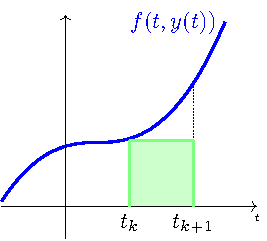
\includegraphics[width=4.47904368358914cm,height=4.05467007739735cm]{k1-7.pdf}}}
    \]
    \item \tmtextit{{\underline{Implizites Euler-Verfahren}}:}
    
    \tmtextit{F{\"u}r $k \in \{ 0, \ldots, K - 1 \}$ lose die folgenden
    nicht-lineare Gleichungssystem nach} $y_{k + 1}$:
    \[ y_{k + 1} = y_k + \tau f (t_{k + 1}, y_{k + 1}) . \]
    \[ \tmscriptoutput{graph}{Graph}{\
       
       \begin{tmcode}
       \tmverbatim{\% \tmop{pdflatex}}
       \end{tmcode}
       
       \begin{tmcode}
       \tmverbatim{\backslash \tmop{textbackslash} \tmop{documentclass}
       \backslash\{\tmop{standalone} \backslash\}}
       \end{tmcode}
       
       \begin{tmcode}
       \tmverbatim{\backslash \tmop{textbackslash} \tmop{usepackage}
       \backslash\{\tmop{tikz} \backslash\}}
       \end{tmcode}
       
       \begin{tmcode}
       \tmverbatim{\backslash \tmop{textbackslash} \tmop{usepackage}
       \backslash\{\tmop{amssymb} \backslash\}}
       \end{tmcode}
       
       \begin{tmcode}
       \tmverbatim{\backslash \tmop{textbackslash} \tmop{usepackage}
       \backslash\{\tmop{amsmath} \backslash\}}
       \end{tmcode}
       
       \begin{tmcode}
       \tmverbatim{\backslash \tmop{textbackslash} \tmop{usepackage}
       \backslash\{\tmop{quiver} \backslash\}}
       \end{tmcode}
       
       \begin{tmcode}
       \tmverbatim{\backslash \tmop{textbackslash} \tmop{usepackage}
       \backslash\{\tmop{mathrsfs} \backslash\}}
       \end{tmcode}
       
       \begin{tmcode}
       \tmverbatim{\backslash \tmop{textbackslash} \tmop{begin}
       \backslash\{\tmop{document} \backslash\}}
       \end{tmcode}
       
       \begin{tmcode}
       \tmverbatim{\backslash \tmop{textbackslash} \tmop{begin}
       \backslash\{\tmop{tikzpicture} \backslash\}}
       \end{tmcode}
       
       \begin{tmcode}
       \tmverbatim{\% \tmop{draw} a \tmop{rechtangle}}
       \end{tmcode}
       
       \begin{tmcode}
       \tmverbatim{\backslash \tmop{textbackslash} \tmop{filldraw}
       [\tmop{fill} = \tmop{green} !20! \tmop{white}, \tmop{draw} =
       \tmop{green} !40! \tmop{white}] (0.5, - 1) \tmop{rectangle} (1.5,
       0.918) ;}
       \end{tmcode}
       
       \begin{tmcode}
       \tmverbatim{\% \tmop{drawing} \tmop{coordinate} \tmop{axis}
       \tmop{lines}}
       \end{tmcode}
       
       \begin{tmcode}
       \tmverbatim{\backslash \tmop{textbackslash} \tmop{draw} [- >] (- 1.5, -
       1) - - (2.5, - 1) \tmop{node} [\tmop{left}, \tmop{below}, \tmop{font}
       =\backslash \tmop{textbackslash}
       \tmop{tiny}]\backslash\{\$t\$\backslash\};}
       \end{tmcode}
       
       \begin{tmcode}
       \tmverbatim{\backslash \tmop{textbackslash} \tmop{draw} [- >] (- 0.5, -
       1.5) - - (- 0.5, 2) \tmop{node} [\tmop{above}, \tmop{font} =\backslash
       \tmop{textbackslash} \tmop{tiny}]\backslash\{\backslash\};}
       \end{tmcode}
       
       \begin{tmcode}
       \tmverbatim{\% \tmop{drawing} \tmop{the} \tmop{straight} \tmop{lines}}
       \end{tmcode}
       
       \begin{tmcode}
       \tmverbatim{\backslash \tmop{textbackslash} \tmop{draw} [\tmop{densely}
       \tmop{dotted}] (1.5, - 1) - - (1.5, 0.918) \tmop{node} [\tmop{above},
       \tmop{font} =\backslash \tmop{textbackslash}
       \tmop{tiny}]\backslash\{\backslash\};}
       \end{tmcode}
       
       \begin{tmcode}
       \tmverbatim{\backslash \tmop{textbackslash} \tmop{draw} [\tmop{color} =
       \tmop{green} !50! \tmop{white}, \tmop{line} \tmop{width} = 1 \tmop{pt}]
       (0.5, - 1) - - (0.5, 0.918) \tmop{node} [\tmop{above}, \tmop{font}
       =\backslash \tmop{textbackslash} \tmop{tiny}]\backslash\{\backslash\};}
       \end{tmcode}
       
       \begin{tmcode}
       \tmverbatim{\backslash \tmop{textbackslash} \tmop{draw} [\tmop{color} =
       \tmop{green} !50! \tmop{white}, \tmop{line} \tmop{width} = 1 \tmop{pt}]
       (1.5, - 1) - - (1.5, 0.918) \tmop{node} [\tmop{above}, \tmop{font}
       =\backslash \tmop{textbackslash} \tmop{tiny}]\backslash\{\backslash\};}
       \end{tmcode}
       
       \begin{tmcode}
       \tmverbatim{\backslash \tmop{textbackslash} \tmop{draw} [\tmop{color} =
       \tmop{green} !50! \tmop{white}, \tmop{line} \tmop{width} = 1 \tmop{pt}]
       (0.5, 0.918) - - (1.5, 0.918) \tmop{node} [\tmop{above}, \tmop{font}
       =\backslash \tmop{textbackslash} \tmop{tiny}]\backslash\{\backslash\};}
       \end{tmcode}
       
       \begin{tmcode}
       \tmverbatim{\% \tmop{drawing} \tmop{functions}}
       \end{tmcode}
       
       \begin{tmcode}
       \tmverbatim{\backslash \tmop{textbackslash} \tmop{draw} [\tmop{color} =
       \tmop{blue}, \tmop{line} \tmop{width} = 1 \tmop{pt}, \tmop{domain} = -
       1.5 : 2] \tmop{plot} (\backslash \tmop{textbackslash} x, \backslash\{1
       / 3\backslash \tmop{textbackslash} x (5 / 2)\backslash\}) \tmop{node}
       [\tmop{left}]\backslash\{\$f (t, y (t))\$\backslash\};}
       \end{tmcode}
       
       \begin{tmcode}
       \tmverbatim{\% \tmop{noting} \tmop{points} \tmop{on} \tmop{axis}}
       \end{tmcode}
       
       \begin{tmcode}
       \tmverbatim{\backslash \tmop{textbackslash} \tmop{draw} (0.5, - 1)
       \tmop{node} [\tmop{below}]\backslash\{\$t\_k\$\backslash\};}
       \end{tmcode}
       
       \begin{tmcode}
       \tmverbatim{\backslash \tmop{textbackslash} \tmop{draw} (1.5, - 1)
       \tmop{node} [\tmop{below}]\backslash\{\$t\_\backslash\{k +
       1\backslash\}\$\backslash\};}
       \end{tmcode}
       
       \begin{tmcode}
       \tmverbatim{\backslash \tmop{textbackslash} \tmop{end}
       \backslash\{\tmop{tikzpicture} \backslash\}}
       \end{tmcode}
       
       \begin{tmcode}
       \tmverbatim{\backslash \tmop{textbackslash} \tmop{end}
       \backslash\{\tmop{document} \backslash\}}
       \end{tmcode}}{\raisebox{-0.00207061107291625\height}{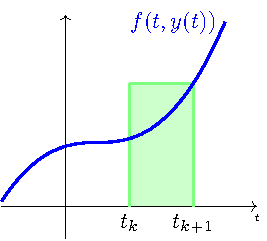
\includegraphics[width=4.47904368358914cm,height=4.05467007739735cm]{k1-8.pdf}}}
    \]
  \end{enumerateroman}
\end{definition}

\begin{remark*}
  {\tmdummy}
  
  \begin{itemizedot}
    \item \tmtextbf{}{\underline{\tmtextit{Geometrische}
    \tmtextit{Interpretation}}} explizites Euler-Verfahrens:
    
    Das explizite Euler-Verfahren kann als Polygonzugverfahren interpretiert
    werden, denn $f (t_k, y_k)$ ist aktuelle ,,Geschwindigkeit`` im
    Phasenraum. Die approximierende L{\"o}sungsmenge geht also von aktueller
    Position $y_k$ um $\tau$ in Richung aktueller Geschwindigkeit:
    
    
    \[ \tmscriptoutput{graph}{Graph}{\
       
       \begin{tmcode}
       \tmverbatim{\% \tmop{pdflatex}}
       \end{tmcode}
       
       \begin{tmcode}
       \tmverbatim{\backslash \tmop{textbackslash} \tmop{documentclass}
       \backslash\{\tmop{standalone} \backslash\}}
       \end{tmcode}
       
       \begin{tmcode}
       \tmverbatim{\backslash \tmop{textbackslash} \tmop{usepackage}
       \backslash\{\tmop{tikz} \backslash\}}
       \end{tmcode}
       
       \begin{tmcode}
       \tmverbatim{\backslash \tmop{textbackslash} \tmop{usepackage}
       \backslash\{\tmop{amssymb} \backslash\}}
       \end{tmcode}
       
       \begin{tmcode}
       \tmverbatim{\backslash \tmop{textbackslash} \tmop{usepackage}
       \backslash\{\tmop{amsmath} \backslash\}}
       \end{tmcode}
       
       \begin{tmcode}
       \tmverbatim{\backslash \tmop{textbackslash} \tmop{usepackage}
       \backslash\{\tmop{quiver} \backslash\}}
       \end{tmcode}
       
       \begin{tmcode}
       \tmverbatim{\backslash \tmop{textbackslash} \tmop{usepackage}
       \backslash\{\tmop{mathrsfs} \backslash\}}
       \end{tmcode}
       
       \begin{tmcode}
       \tmverbatim{\backslash \tmop{textbackslash} \tmop{begin}
       \backslash\{\tmop{document} \backslash\}}
       \end{tmcode}
       
       \begin{tmcode}
       \tmverbatim{\backslash \tmop{textbackslash} \tmop{begin}
       \backslash\{\tmop{tikzpicture} \backslash\}}
       \end{tmcode}
       
       \begin{tmcode}
       \tmverbatim{\% \tmop{draw} \tmop{coordinate} \tmop{axis} \tmop{lines}}
       \end{tmcode}
       
       \begin{tmcode}
       \tmverbatim{\backslash \tmop{textbackslash} \tmop{draw} [- >] (- 0.4,
       0) - - (4.4, 0) \tmop{node} [\tmop{left}, \tmop{below}, \tmop{font}
       =\backslash \tmop{textbackslash} \tmop{tiny}]\backslash\{\backslash\};}
       \end{tmcode}
       
       \begin{tmcode}
       \tmverbatim{\backslash \tmop{textbackslash} \tmop{draw} [- >] (0, -
       0.4) - - (0, 3.4) \tmop{node} [\tmop{above}, \tmop{font} =\backslash
       \tmop{textbackslash} \tmop{tiny}]\backslash\{\backslash\};}
       \end{tmcode}
       
       \begin{tmcode}
       \tmverbatim{\% \tmop{draw} \tmop{the} \tmop{red} \tmop{curve}}
       \end{tmcode}
       
       \begin{tmcode}
       \tmverbatim{\backslash \tmop{textbackslash} \tmop{draw} [\tmop{color} =
       \tmop{red}, \tmop{line} \tmop{width} = 1 \tmop{pt}, \tmop{domain} = 2 :
       3] \tmop{plot} (\backslash \tmop{textbackslash} x, \backslash\{1.8 -
       \tmop{sqrt} (1 - (\backslash \tmop{textbackslash} x - 2)
       2)\backslash\}) \tmop{node} [\tmop{left}]\backslash\{\$y
       (t)\$\backslash\};}
       \end{tmcode}
       
       \begin{tmcode}
       \tmverbatim{\backslash \tmop{textbackslash} \tmop{draw} [\tmop{color} =
       \tmop{red}, \tmop{line} \tmop{width} = 1 \tmop{pt}, \tmop{domain} = 1.1
       : 3] \tmop{plot} (\backslash \tmop{textbackslash} x, \backslash\{1.7 +
       \tmop{sqrt} (1 - (\backslash \tmop{textbackslash} x - 2)
       2)\backslash\}) \tmop{node} [\tmop{above}]\backslash\{\backslash\};}
       \end{tmcode}
       
       \begin{tmcode}
       \tmverbatim{\% \tmop{draw} \tmop{the} \tmop{arrow} \tmop{of} \tmop{the}
       \tmop{red} \tmop{curve}}
       \end{tmcode}
       
       \begin{tmcode}
       \tmverbatim{\backslash \tmop{textbackslash} \tmop{foreach} \backslash
       \tmop{textbackslash} x /\backslash \tmop{textbackslash} \tmop{angle}
       \tmop{in} \backslash\{1.13 / 245\backslash\}\backslash\{\backslash
       \tmop{textbackslash} \tmop{foreach} \backslash \tmop{textbackslash} y
       \tmop{in} \backslash\{2.2\backslash\}\backslash\{\backslash
       \tmop{textbackslash} \tmop{draw} [- >, \tmop{thick}, \tmop{color} =
       \tmop{red}] (\backslash \tmop{textbackslash} x, \backslash
       \tmop{textbackslash} y) - - + (\backslash \tmop{textbackslash}
       \tmop{angle} : 0.2) ; \backslash\}\backslash\}}
       \end{tmcode}
       
       \begin{tmcode}
       \tmverbatim{\\
       }
       \end{tmcode}
       
       \begin{tmcode}
       \tmverbatim{\\
       }
       \end{tmcode}
       
       \begin{tmcode}
       \tmverbatim{\% \tmop{draw} \tmop{the} \tmop{vector} \tmop{field}
       \tmop{name}}
       \end{tmcode}
       
       \begin{tmcode}
       \tmverbatim{\backslash \tmop{textbackslash} \tmop{draw} [\tmop{color} =
       \tmop{blue}] (2, 0.8) \tmop{node}
       [\tmop{below}]\backslash\{\$y\_\backslash\{k + 1\backslash\}= y\_k
       +\backslash \tmop{textbackslash} \tmop{tau} f (t\_k,
       y\_k)\$\backslash\};}
       \end{tmcode}
       
       \begin{tmcode}
       \tmverbatim{\% \tmop{draw} \tmop{the} \tmop{vector} \tmop{field}
       \tmop{arrows}}
       \end{tmcode}
       
       \begin{tmcode}
       \tmverbatim{\backslash \tmop{textbackslash} \tmop{foreach} \backslash
       \tmop{textbackslash} x /\backslash \tmop{textbackslash} \tmop{angle}
       \tmop{in} \backslash\{2 / 7\backslash\}\backslash\{\backslash
       \tmop{textbackslash} \tmop{foreach} \backslash \tmop{textbackslash} y
       \tmop{in} \backslash\{0.78\backslash\}\backslash\{\backslash
       \tmop{textbackslash} \tmop{draw} [- >, \tmop{color} = \tmop{blue}]
       (\backslash \tmop{textbackslash} x, \backslash \tmop{textbackslash} y)
       - - + (\backslash \tmop{textbackslash} \tmop{angle} : 0.5) ;
       \backslash\}\backslash\}}
       \end{tmcode}
       
       \begin{tmcode}
       \tmverbatim{\backslash \tmop{textbackslash} \tmop{foreach} \backslash
       \tmop{textbackslash} x /\backslash \tmop{textbackslash} \tmop{angle}
       \tmop{in} \backslash\{2.5 / 35\backslash\}\backslash\{\backslash
       \tmop{textbackslash} \tmop{foreach} \backslash \tmop{textbackslash} y
       \tmop{in} \backslash\{0.85\backslash\}\backslash\{\backslash
       \tmop{textbackslash} \tmop{draw} [- >, \tmop{color} = \tmop{blue}]
       (\backslash \tmop{textbackslash} x, \backslash \tmop{textbackslash} y)
       - - + (\backslash \tmop{textbackslash} \tmop{angle} : 0.55) ;
       \backslash\}\backslash\}}
       \end{tmcode}
       
       \begin{tmcode}
       \tmverbatim{\backslash \tmop{textbackslash} \tmop{foreach} \backslash
       \tmop{textbackslash} x /\backslash \tmop{textbackslash} \tmop{angle}
       \tmop{in} \backslash\{2.95 / 65\backslash\}\backslash\{\backslash
       \tmop{textbackslash} \tmop{foreach} \backslash \tmop{textbackslash} y
       \tmop{in} \backslash\{1.15\backslash\}\backslash\{\backslash
       \tmop{textbackslash} \tmop{draw} [- >, \tmop{color} = \tmop{blue}]
       (\backslash \tmop{textbackslash} x, \backslash \tmop{textbackslash} y)
       - - + (\backslash \tmop{textbackslash} \tmop{angle} : 0.6) ;
       \backslash\}\backslash\}}
       \end{tmcode}
       
       \begin{tmcode}
       \tmverbatim{\backslash \tmop{textbackslash} \tmop{foreach} \backslash
       \tmop{textbackslash} x /\backslash \tmop{textbackslash} \tmop{angle}
       \tmop{in} \backslash\{3.2 / 95\backslash\}\backslash\{\backslash
       \tmop{textbackslash} \tmop{foreach} \backslash \tmop{textbackslash} y
       \tmop{in} \backslash\{1.7\backslash\}\backslash\{\backslash
       \tmop{textbackslash} \tmop{draw} [- >, \tmop{color} = \tmop{blue}]
       (\backslash \tmop{textbackslash} x, \backslash \tmop{textbackslash} y)
       - - + (\backslash \tmop{textbackslash} \tmop{angle} : 0.65) ;
       \backslash\}\backslash\}}
       \end{tmcode}
       
       \begin{tmcode}
       \tmverbatim{\backslash \tmop{textbackslash} \tmop{foreach} \backslash
       \tmop{textbackslash} x /\backslash \tmop{textbackslash} \tmop{angle}
       \tmop{in} \backslash\{3.15 / 125\backslash\}\backslash\{\backslash
       \tmop{textbackslash} \tmop{foreach} \backslash \tmop{textbackslash} y
       \tmop{in} \backslash\{2.35\backslash\}\backslash\{\backslash
       \tmop{textbackslash} \tmop{draw} [- >, \tmop{color} = \tmop{blue}]
       (\backslash \tmop{textbackslash} x, \backslash \tmop{textbackslash} y)
       - - + (\backslash \tmop{textbackslash} \tmop{angle} : 0.7) ;
       \backslash\}\backslash\}}
       \end{tmcode}
       
       \begin{tmcode}
       \tmverbatim{\backslash \tmop{textbackslash} \tmop{foreach} \backslash
       \tmop{textbackslash} x /\backslash \tmop{textbackslash} \tmop{angle}
       \tmop{in} \backslash\{2.75 / 155\backslash\}\backslash\{\backslash
       \tmop{textbackslash} \tmop{foreach} \backslash \tmop{textbackslash} y
       \tmop{in} \backslash\{2.9\backslash\}\backslash\{\backslash
       \tmop{textbackslash} \tmop{draw} [- >, \tmop{color} = \tmop{blue}]
       (\backslash \tmop{textbackslash} x, \backslash \tmop{textbackslash} y)
       - - + (\backslash \tmop{textbackslash} \tmop{angle} : 0.75) ;
       \backslash\}\backslash\}}
       \end{tmcode}
       
       \begin{tmcode}
       \tmverbatim{\backslash \tmop{textbackslash} \tmop{foreach} \backslash
       \tmop{textbackslash} x /\backslash \tmop{textbackslash} \tmop{angle}
       \tmop{in} \backslash\{2.1 / 195\backslash\}\backslash\{\backslash
       \tmop{textbackslash} \tmop{foreach} \backslash \tmop{textbackslash} y
       \tmop{in} \backslash\{3.2\backslash\}\backslash\{\backslash
       \tmop{textbackslash} \tmop{draw} [- >, \tmop{color} = \tmop{blue}]
       (\backslash \tmop{textbackslash} x, \backslash \tmop{textbackslash} y)
       - - + (\backslash \tmop{textbackslash} \tmop{angle} : 0.8) ;
       \backslash\}\backslash\}}
       \end{tmcode}
       
       \begin{tmcode}
       \tmverbatim{\backslash \tmop{textbackslash} \tmop{foreach} \backslash
       \tmop{textbackslash} x /\backslash \tmop{textbackslash} \tmop{angle}
       \tmop{in} \backslash\{1.35 / 225\backslash\}\backslash\{\backslash
       \tmop{textbackslash} \tmop{foreach} \backslash \tmop{textbackslash} y
       \tmop{in} \backslash\{3\backslash\}\backslash\{\backslash
       \tmop{textbackslash} \tmop{draw} [- >, \tmop{color} = \tmop{blue}]
       (\backslash \tmop{textbackslash} x, \backslash \tmop{textbackslash} y)
       - - + (\backslash \tmop{textbackslash} \tmop{angle} : 0.85) ;
       \backslash\}\backslash\}}
       \end{tmcode}
       
       \begin{tmcode}
       \tmverbatim{\backslash \tmop{textbackslash} \tmop{end}
       \backslash\{\tmop{tikzpicture} \backslash\}}
       \end{tmcode}
       
       \begin{tmcode}
       \tmverbatim{\backslash \tmop{textbackslash} \tmop{end}
       \backslash\{\tmop{document} \backslash\}}
       \end{tmcode}}{\raisebox{-0.00196250541413847\height}{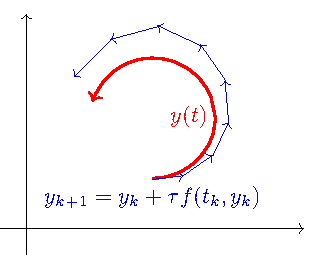
\includegraphics[width=5.22274695001968cm,height=4.27802374393283cm]{k1-9.pdf}}}
    \]
    \item {\underline{\tmtextit{Rechenaufwand}}} implizites Euler-Verfahrens:
    
    Das implizite Euler-Verfahren erfordert L{\"o}sung eines nicht-linearen
    Gleichungssystems in jedem Schritt, typischerweise z.B. mittels
    Newton-Verfahren. Dies ist aufwendiger als einzelne $f$-Auswertung im
    expliziten Euler-Verfahren. Als Startwert f{\"u}r Newton kann z.B. alter
    Wert $y_k$ verwendet werden. Wegen der i.A. lokalen Konvergenz von Newton
    sollte $\tau$ nicht zu gro{\ss} gew{\"a}hlt werden. 
  \end{itemizedot}
\end{remark*}

\begin{example*}
  (Euler-Verfahren f{\"u}r R{\"a}uber-Beute-Modell)
  \[ \tmop{hier} \tmop{kommt} \tmop{noch} \tmop{ein} \tmop{Bild} \tmop{aus}
     \tmop{Uebungsaufgabe} \tmop{PB} 1 \upright{A} 2 \]
  Aus dem Bild sehen wir:
  \begin{itemizedot}
    \item Explizites Euler: Gr{\"o}{\ss}eres $\tau$ liefert schnelleres
    Verfahren, aber Spiralen divergieren nach au{\ss}en und keine
    Periozit{\"a}t beobachtbar.
    
    \item Implizites Euler liefert auch Spiralen, die im Fixpunkt laufen,
    aber auch keine Periozit{\"a}t beobachtbar. 
  \end{itemizedot}
\end{example*}

Verbesserungen von Euler-Verfahren sind m{\"o}glich durch bessere Quadraturen,
z.B. mit der Trapezregel
\begin{equation}
  Q_1 (f) = \frac{\tau}{2} [f (t_k, y (t_k)) + f (t_{k + 1}, y (t_{k + 1}))] .
\end{equation}
Eine Wahl von $f (t_{k + 1}, y (t_{k + 1}))$ durch explizites Euler Verfahren
liefert:

\begin{definition}
  \tmtextbf{(Explizites Verfahren von Heun)}
  
  \tmtextit{F{\"u}r $k \in \{ 0, \ldots, K - 1 \}$ setze
  \[ y_{k + 1} \assign y_k + \frac{\tau}{2} (f_0 + f_1) \]
  $\text{mit\quad} f_0 \assign f (t_k, y_k) \quad \text{und\quad} f_1 \assign
  f (t_{k + 1}, y_k + \tau f (t_k, y_k)) .$}
\end{definition}

Eine Wahl $f (t_{k + 1}, y (t_{k + 1})) \approx f (t_{k + 1}, y_{k + 1})$
liefert in (1.13):

\begin{definition}
  \tmtextbf{(Crank-Nicolson-Verfahren)}
  
  \tmtextit{F{\"u}r $k \in \{ 0, \ldots, K - 1 \}$ l{\"o}se das nicht-lineare
  Gleichungssystem}
  \[ y_{k + 1} = y_k + \frac{\tau}{2} (f (t_k, y_k) + f (t_{k + 1}, y_{k +
     1})) . \]
\end{definition}

Das Crank-Nicolson-Verfahren, sowie das explizite und implizite
Euler-Verfahren, sind Spezialf{\"a}lle des
{\underline{\tmtextit{$\theta$-Verfahrens}}}, bei dem $\theta \in [0, 1]$ eine
Gewichtung des expliziten und impliziten Anteils mit Gewichten $\theta$ bzw.
$(1 - \theta)$ gew{\"a}hlt werden.

\

W{\"a}hrend das explizite Euler oder Heun-Verfahren f{\"u}r jedes $\tau > 0$
wohldefinierte Iterierte besitzen (solange die Argumente von $f$ in $D$
liegen), m{\"u}ssen bei {\underline{\tmtextit{impliziten Verfahren}}} in der
Regel {\underline{\tmtextit{Zeitschrittweiten-Beschr{\"a}nkungen}}} erfolgen,
{\underline{\tmtextit{damit}}} das \tmtextit{{\underline{Verfahren
wohldefiniert}}} ist.

Wir zeigen dies f{\"u}r das implizite Euler-Verfahren nach zwei
Hilfsaussagen:

\begin{theorem}
  \tmtextbf{(Brouwer'scher Fixpunktsatz)}
  
  \tmtextit{Sei} $B \assign \overline{B_1 (0)} \subseteq \mathbb{R}^d$
  \tmtextit{die abgeschlossene Einheitskugel und $h : B \rightarrow B$
  stetig.}
  
  \tmtextit{Dann besitzt $h$ einen Fixpunkt in $B$, d.h. $\exists x^{\ast} \in
  B : h (x^{\ast}) = x^{\ast}$}.
\end{theorem}

Der Brouwer'scher Fixpunktsatz verlangt schw{\"a}chere Bedingung von der
Funktion als Banach'scher Fixpunktsatz. Damit kann man zwar f{\"u}r eine
gr{\"o}{\ss}ere Klasse von Funktionen die Existenz eines Fixpunkts nachweisen,
aber man hat das iterative Konvergenzverfahren zur Bestimmung des Fixpunkts
nicht mehr.

\begin{proof}
  (aus Topologie von Prof. Eisermann)
  
  Gegenannahme: Es gilt $f (x) \neq x$ f{\"u}r alle $x \in B$.
  
  Zu jedes $x \in B$ existiert genau ein $t \in \mathbb{R}_+$ so dass $r (x)
  = f (x) + t (x - f (x))$ \ in $\partial B$ liegt. Dies de\textbackslash
  niert eine stetige Abbildung $r : B \rightarrow \partial \tmmathbf{} B$.
  F{\"u}r jedes $x \in \partial B$ gilt $r (x) = x$, also ist $r$ eine
  Retraktion von $B$ auf $\partial B$ . Das ist aber unm{\"o}glich, also muss
  $f$ mindestens einen Fixpunkt haben.
\end{proof}

\begin{corollary}
  \tmtextbf{(Existenz von Nullstelle)}
  
  \tmtextit{Sei $B_{\delta} \assign \overline{B_{\delta} (0)} \subset
  \mathbb{R}^d$ der abgeschlossene Ball mit Radius $\delta \in \mathbb{R}_+$
  um $0$.
  
  Sei $g : B_{\delta} \rightarrow \mathbb{R}^d$ stetig mit
  \[ \forall x \in \partial B_{\delta} : \text{\quad} \langle g (x), x
     \rangle \geq 0. \]
  {\hspace{1.7em}}Dann besitzt $g$ (mindestens) eine Nullstelle in
  $B_{\delta}$.}
\end{corollary}

\begin{proof}
  wieder durch Widerspruch:
  
  Angenommen, $\forall x \in B_{\delta} : g (x) \neq 0.$
  
  Definiere eine Normalisierungsabbildung auf Einheitskugel:
  \[ h : B_1 \rightarrow B_1, y \mapsto - \frac{g (\delta y)}{\parallel g
     (\delta y) \parallel} . \]
  {\hspace{1.7em}}$h$ ist wohldefiniert und stetig.
  
  Mit Brouwer'schem Fixpunktsatz existiert ein $y^{\ast } \in B_1$ mit
  $y^{\ast } = h (y^{\ast })$ und somit
  \[ x^{\ast } \assign \delta y^{\ast } = - \frac{\delta g (x^{\ast
     })}{\parallel g (x^{\ast }) \parallel} \in \partial B_{\delta} . \]
  {\hspace{1.7em}}Aber
  \[ \langle g (x^{\ast }), x^{\ast } \rangle = - \delta \frac{\langle g
     (x^{\ast }), g (x^{\ast }) \rangle}{\parallel g (x^{\ast }) \parallel} =
     - \delta \parallel g (x^{\ast }) \parallel < 0 \]
  ist ein Widerspruch zur Voraussetzung.
\end{proof}

Mit obigen Vorbereitungen kommen wir nun zur Wohldefiniertheit des impliziten
Euler-Verfahrens:

\begin{theorem}
  \tmtextbf{(Existenz und Eindeutigkeit der impliziten Euler-Iterierten)}
  
  \tmtextit{Sei $D = I \times \mathbb{R}^d$ ein Gebiet.
  
  Sei $f : D \rightarrow \mathbb{R}^d$ stetig und erf{\"u}lle die
  ,,{\underline{einseitige Lipschitz-Bedingung}}``
  \[ \exists L \in \mathbb{R} \enspace \forall (t, x), (t, y) \in D :
     \text{\quad} \langle f (t, x) - f (t, y), x - y \rangle \leq L \parallel
     x - y \parallel^2 . \]
  {\hspace{1.7em}}Falls $\tau L < 1$, dann hat die nicht-lineare Gleichung
  \[ y_{k + 1} = y_k + \tau f (t_{k + 1}, y_{k + 1}) \]
  genau eine L{\"o}sung $y_{k + 1}$ zu gegebenem $y_k$.}
\end{theorem}

\begin{proof}
  Zur Existenz der L{\"o}sung:
  
  Gesucht ist also eine Nullstelle $y_{k + 1}$ von stetiger Funktion
  \[ g (y) \assign y - (y_k + \tau f (t_{k + 1}, y)) \quad \text{f{\"u}r} y
     \in \mathbb{R}^d . \]
  {\hspace{1.7em}}Die einseitige Lipschitz-Bedingung liefert
  \begin{eqnarray*}
    \langle g (x) - g (y), x - y \rangle & = & \langle x - y_k - \tau f (t_{k
    + 1}, x) - y + y_k + \tau f (t_{k + 1}, y), x - y \rangle\\
    & = & \parallel x - y \parallel^2 - \tau \langle f (t_{k + 1}, x) - f
    (t_{k + 1}, y), x - y \rangle\\
    & \geq & \parallel x - y \parallel^2 - \tau \hspace{4em} L \parallel x -
    y \parallel^2\\
    & = & (1 - \tau L) \parallel x - y \parallel^2 .
  \end{eqnarray*}
  {\hspace{1.7em}}Wegen $\tau L < 1$ ist $c \assign 1 - \tau L > 0$, und wir
  erhalten:
  \begin{equation}
    \langle g (x) - g (y), x - y \rangle \geq c \parallel x - y \parallel^2 .
  \end{equation}
  {\hspace{1.7em}}Setze $y = 0$ in (1.14) und erhalte:
  \begin{eqnarray*}
    \langle g (x), x \rangle & = & \langle g (x) - g (0), x - 0 \rangle +
    \langle g (0), x - 0 \rangle\\
    & \geq & \langle g (x) - g (0), x - 0 \rangle + (- \parallel g (0)
    \parallel \cdot \parallel x \parallel)\\
    & \geq & \text{{\hspace{3em}}} c \parallel x - 0 \parallel^2
    \text{{\hspace{2.7em}}} - \parallel g (0) \parallel \cdot \parallel x
    \parallel\\
    & = & \parallel x \parallel (c \parallel x \parallel - \parallel g (0)
    \parallel)
  \end{eqnarray*}
  wobei die 2. Zeile aus Cauchy-Schwarz-Ungleichung und 3. Zeile aus (1.14)
  folgen.
  
  F{\"u}r jedes $\delta \geq \frac{\parallel g (0) \parallel}{c}$ und jedes $x
  \in \partial B_{\delta}$ gilt dann $\langle g (x), x \rangle \geq 0$.
  
  Dank 1.13 existiert mindestens eine Nullstelle $x \in B_{\delta}$.
  
  {\hspace{3em}}Zur Eindeutigkeit der L{\"o}sung:
  
  Seien $x_1$, $x_2 \in B_{\delta}$ Nullstellen von $g$, dann gilt
  \[ 0 = \langle 0, x_1 - x_2 \rangle = \langle g (x_1) - g (x_2), x_1 - x_2
     \rangle \geq c \parallel x_1 - x_2 \parallel^2 \]
  und damit muss $x_1 = x_2$ sein. 
\end{proof}

\begin{remark*}
  \tmtextbf{(Einseitige Lipschitz-Bedingung)}
  \begin{itemizedot}
    \item {\underline{\tmtextit{Einseitige Lipschitz-Bedingung}}} ist
    {\underline{\tmtextit{Abschw{\"a}chung}}} der Lipschitz-Stetigkeit:
    
    $f$ Lipschitz-stetig im 2. Arg.\enspace$\Rightarrow$\enspace$f$
    erf{\"u}llt einseitige Lipschitz-Bedingung:
    \[ \langle f (t, x) - f (t, y), x - y \rangle \leq \parallel f (t, x) - f
       (t, y) \parallel \cdot \parallel x - y \parallel \leq L \parallel x - y
       \parallel^2 . \]
    \item Es gibt Funktionen, welche die einseitige Lipschitz-Bedingung
    erf{\"u}llen, aber Lipschitz-stetig bzgl. einem gr{\"o}{\ss}eren/anderen
    $L$oder sogar nicht Lipschitz-stetig sind:
    \begin{itemizedot}
      \item $f (t, y) = - y$ erf{\"u}llt die einseitige Lipschitz-Bedingung
      mit $L = - 1$, aber $f$ ist Lipschitz-stetig bzgl. $y$ mit
      Lipschitz-Konstante $1$.
      
      \item $f (t, y) = - y^3$ erf{\"u}llt die einseitige Lipschitz-Bedingung
      mit $L = 0$, aber $f$ ist nicht Lipschitz-stetig als Funktion auf $I
      \times \mathbb{R}$.
    \end{itemizedot}
  \end{itemizedot}
\end{remark*}

Als n{\"a}chstes verwllgemeinern wir das Einschritt-Verfahren:

\begin{definition}
  \tmtextbf{(Allgemeines Einschritt-Verfahren)}
  
  \tmtextit{Sei ein AWP gem{\"a}{\ss} Definition 1.2 gegeben und oBdA $I = [0,
  T]$ f{\"u}r ein $T \in \mathbb{R}_+$.
  
  F{\"u}r ein $K \in \mathbb{N}$ seien Zeitpunkte $0 = : t_0 < t_1 < \cdots <
  t_K \assign T$ zu {\underline{Gitter}} $\Delta \assign \{ t_0, \ldots, t_K
  \}$ mit lokalen Schrittweiten $\tau_k \assign t_{k + 1} - t_k$ mit $k \in \{
  0, \ldots, K - 1 \}$ gegeben.
  
  Ein Verfahren der Form
  \[ \forall k \in \{ 0, \ldots, K - 1 \} : \text{\quad} y_{k + 1} : = y_k +
     \tau_k \phi (t_k, \tau_k, y_k, y_{k + 1}) \]
  hei{\ss}t {\underline{Einschrittverfahren (ESV) mit Verfahrensfunktion
  $\phi$}}, die als stetig vorausgesetzt wird. \ }
  
  \tmtextit{Falls $\phi$ nicht von $y_{k + 1}$ abh{\"a}ngt, hei{\ss}t das
  Verfahren {\underline{explizit}}, und wir schreiben abk{\"u}rzend $\phi
  (t_k, \tau_k, y_k)$; sonst hei{\ss}t das Verfahren {\underline{implizit}}.}
\end{definition}

Also ist explizites / implizites Euler-Verfahren aus Definition 1.9 \
Spezialart vom Einschrittverfahren.

Wir vereinbaren noch folgende \tmtextbf{Notationen}:
\begin{itemizedot}
  \item $\{ y_k \}_{k = 0}^K$ k{\"o}nnen als
  {\underline{\tmtextit{Gitterfunktion}}} $y_{\Delta} : \Delta \rightarrow
  \mathbb{R}^d$ interpretiert werden, in dem man $y_{\Delta} (t_k) \assign
  y_k$ setzt.
  
  \item Wir definieren die {\underline{\tmtextit{Gitterweite}}} eines Gitters
  $\Delta \assign \{ t_0, \ldots, t_K \}$ als
  \[ \tau_{\Delta} \assign \max_{k \in \{ 0, \ldots, K - 1 \}} \tau_k . \]
  \item Sei $y : I \rightarrow \mathbb{R}^d$ eine L{\"o}sung des AWP. Unser
  Ziel ist eine Approximation $y (t_k) \approx y_k$, daher definieren wir zu
  einem Gitter $\Delta \assign \{ t_0, \ldots, t_K \}$ die
  {\underline{\tmtextit{Fehlerfunktion}}} $e_{\Delta} : \Delta \rightarrow
  \mathbb{R}^d$ mit
  \[ \forall k \in \{ 0, \ldots, K \} : \text{\quad} e_{\Delta} (t_k) = e_k
     \assign y_k - y (t_k) \]
  sowie eine {\underline{\tmtextit{Gitternorm}}}
  \[ \parallel e_{\Delta} \parallel_{\Delta} \assign \max_{k \in \{ 0, \ldots,
     K \}} \parallel e_k \parallel_2, \]
  damit wir {\"u}ber Fehler und Konvergenz sprechen k{\"o}nnen.
\end{itemizedot}
\begin{definition}
  \tmtextbf{(Konvergenz, Konvergenzordnung)}
  
  \tmtextit{Ein ESV hei{\ss}t {\underline{konvergent}}
  
  $: \Leftrightarrow$ F{\"u}r alle Folgen $(\Delta_K)_{K \in \mathbb{N}}$ mit
  $\tau_{\Delta_K} \xrightarrow{K \rightarrow \infty} 0$ gilt
  \[ \lim_{K \rightarrow \infty} \parallel e_{\Delta_K} \parallel_{\Delta} =
     0. \]
  {\hspace{1.7em}}Das ESV hat {\underline{(mindestens) Konvergenzordnung $p
  \in \mathbb{R}_+$}}
  
  $: \Leftrightarrow$ $\exists C \in \mathbb{R}_+$ ${\exists \tau^{\ast}}^{}
  \in \mathbb{R}_+$ $\forall \Delta \text{ mit} \tau_{\Delta} \leq \tau^{\ast}
  :$
  \[ \parallel e_{\Delta} \parallel_{\Delta} \leq C \tau_{\Delta}^p . \]}
\end{definition}

\begin{example*}
  \tmtextbf{(Konv.Ord. des expliziten Euler-Verfahren beim skalaren AWP)}
  
  \tmtextit{\tmtextup{Wir wollen zeigen, dass das explizite Euler-Verfahren
  f{\"u}r lineares skalares AWP mit mind. Ordnung $1$ konvergiert.
  
  Betrachte der Einfachheit halber {\"a}quidistante Gitter $\Delta$ (F{\"u}r
  allgemeine Gitter gilt die Aussage auch, nur wird die Notation
  l{\"a}stiger{\textdots}).
  
  Ein lineares skalares AWP
  \[ y' = \lambda y, \text{\qquad} y (0) = y_0 \]
  hat eine L{\"o}sung $y : \mathbb{R} \rightarrow \mathbb{R}, t \mapsto y_0
  \mathbf{e}^{\lambda t}$.
  
  Auf {\"a}quidistantem Gitter $\Delta \assign \{ 0 = t_0, \ldots, t_K \}$,
  also
  \[ \tau \assign \tau_0 = \tau_1 = \cdots = \tau_{K - 1}, \]
  hat das explizite Euler-Verfahren die Verfahrensfunktion
  \[ \phi (t_k, \tau_k, y_k, y_{k + 1}) = f (y_k, t) = \lambda y_k \]
  und somit liefert es f{\"u}r alle $k \in \{ 0, \ldots, K - 1 \}$:}
  \[ y_{k + 1} = y_k + \tau \lambda y_k = (1 + \tau \lambda) y_k = \cdots = (1
     + \tau \lambda)^{k + 1} y_0 . \]}
  
  {\hspace{1.7em}}Mit Taylor-Entwicklung $1$. Grades auf die
  L{\"o}sungsfunktion $y (t) =\mathbf{e}^{\lambda t}$ um $0$ folgt
  \[ \mathbf{e}^{\lambda t} = 1 + \tau \lambda +\mathcal{O} (\tau^2) . \]
  {\hspace{1.7em}}Also gilt f{\"u}r alle $k \in \{ 0, \ldots, K - 1 \}$:
  \[ y_k = (1 + \tau \lambda)^k y_0 = (\mathbf{e}^{\lambda \tau} +\mathcal{O}
     (\tau^2))^k y_0 = (\mathbf{e}^{\lambda k \tau} +\mathcal{O} (k \tau^2))
     y_0 \]
  wobei die zweite Gleichheit aus binomischer Formel folgt.
  
  Da $\Delta \assign \{ 0 = t_0, \ldots, t_K \} ${\"a}quidistant ist, gilt \
  \[ \mathbf{e}^{\lambda k \tau} =\mathbf{e}^{\lambda t_k}, \]
  und somit
  \[ e_k = y_k -\mathbf{e}^{\lambda t_k} y_0 =\mathcal{O} (k \tau^2) y_0, \]
  welches zusammen mit $K = T / t$ besagt
  \[ \parallel e_{\Delta} \parallel_{\Delta} = \max_{k \in \{ 0, \ldots, K
     \}} \parallel e_k \parallel_2 =\mathcal{O} (K \tau^2) \parallel y_0
     \parallel = T \parallel y_0 \parallel \mathcal{O} (\tau) . \]
  {\hspace{1.7em}}$\Rightarrow$ Man erh{\"a}lt Konvergenzordnung mindestens $p
  = 1$.
\end{example*}

F{\"u}r allgemeine ESV h{\"a}ngt Konvergenz mit dem Begriff der Konsistenz
zusammen:

\begin{definition}
  \tmtextbf{(Konsistenz, Konsistenzordnung)}
  
  \tmtextit{Sei $\phi$ eine Verfahrensfunktion eines ESV zur Approximation von
  L{\"o}sung eines AWP $y' = f (t, y)$ (mit geeigneter AWB), d.h. f{\"u}r
  jedes $k \in \{ 0, \ldots, K - 1 \} $gilt \
  \[ y_{k + 1} = y_k + \tau_k \phi (t_k, \tau_k, y_k, y_{k + 1}) . \]
  {\hspace{1.7em}}Das Verfahren hei{\ss}t {\underline{konsistent}} mit dem
  AWP, g.d.w.
  \[ \forall (t, y) \in D : \text{\qquad} \lim_{\tau \rightarrow \infty} \phi
     (t, \tau, y, y + \tau) = f (t, y) . \]
  {\hspace{1.7em}}F{\"u}r $t, \tau \text{ s.d. } [t, t + \tau] \subseteq I$,
  $y : I \xrightarrow{} \mathbb{R}^d$ eine L{\"o}sung des AWP und $z \in
  \mathbb{R}^d$ eine L{\"o}sung von
  \[ z = y (t) + \tau \phi (t, \tau, y (t), z) \]
  definieren wir den {\underline{Iterationsfehler}}
  \[ \eta (t, \tau) \assign z - y (t + \tau) = y (t) + \tau \phi (t, \tau, y
     (t), z) - y (t + \tau) . \]
  {\hspace{1.7em}}Das Verfahren $\phi$ hei{\ss}t {\underline{konsistent mit
  (mindestens) Ordnung $p \in \mathbb{R}_+$}}
  
  $: \Leftrightarrow$ $\exists C_p \in \mathbb{R}_+$ $\forall t, \tau$ s.d.
  $[t, t + \tau] \subseteq I$:
  \[ \parallel \eta (t, \tau) \parallel \leq C_p \tau^{p + 1} . \]}
\end{definition}

\begin{remark*}
  (zu Definition 1.17)
  \begin{itemizedot}
    \item Die Gr{\"o}{\ss}e $z$ kann man interpretieren als die L{\"o}sung des
    Verfahrens von der exakten L{\"o}sung $y$ zum Zeitpunkt $t$ und
    Schrittweite $\tau$.
    
    \item $\eta$ misst somit, wie sehr ein einzelner Schritt des Verfahrens
    bei exakten Anfangswerten $y (t_k)$ die L{\"o}sung $y (t_{k + 1})$
    verpasst.
    
    \item Es sind {\"a}quivalent
    \[ \eta (t, \tau) =\mathcal{O} (\tau^{p + 1}) \quad \Leftrightarrow
       \text{\quad} \frac{y (t + \tau) - y (t)}{\tau} - \phi (t, \tau, y (t),
       z) =\mathcal{O} (\tau^p) . \]
    Die Gr{\"o}{\ss}e an der rechten Seite nennt man
    {\underline{\tmtextit{Abschneidefehler}}}, oder auf Englisch
    ,,\tmtextit{{\underline{truncation error}}}``.
    
    \item Konsistenzordnung eines ESV ist unter Annahme gewisser
    Differenzierbarkeit von $f$ durch Taylor-Approximation bestimmbar. Die
    Differenzierbarkeit von $f$ {\"u}bertr{\"a}gt sich auf die L{\"o}sung $y$,
    denn $y' = f (t, y)$. 
  \end{itemizedot}
\end{remark*}

\begin{example*}
  \tmtextbf{(Konsistenzordnung der beiden Euler-Verfahren f{\"u}r $d = 1$)}
  
  Sei $d = 1$ und $f \in C^1$, d.h. $y \in C^2$.
  \begin{enumerateroman}
    \item Das {\underline{\tmtextit{explizite Euler-Verfahren}}} lautet
    \[ \phi (t, \tau, y_k, y_{k + 1}) = f (t, y_k) . \]
    $\Rightarrow$ $\phi (t, 0, y, y) = f (t, y)$, also ist das explizite
    Euler-Verfahren konsistent.\qquad  Mit Taylor-Entwicklung $1$. Grades auf
    $y (t + \tau)$ nach $\tau$ folgt
    \[ y (t + \tau) = y (t) + \tau y' (t) + \frac{1}{2} \tau^2 y'' (\xi)
       \quad \text{mit\quad} \xi \in [t, t + \tau] . \]
    Wegen $y' (t) = f (t, y)$ ist
    \[ \eta (t, \tau) = y (t) + \tau f (t, y (t)) - y (t) - \tau f (t, y (t))
       - \frac{1}{2} \tau^2 y'' (\xi) = - \frac{1}{2} \tau^2 y'' (\xi) . \]
    Das bedeutet
    \[ | \eta (t, \tau) | = \left| \frac{\tau^2}{2} y'' (\xi) \right| \leq
       \frac{1}{2} \parallel y'' \parallel_{\infty} \tau^2, \]
    also betr{\"a}gt die Konsistenzordnung von mindestens $p = 1$.
    
    \item Das {\underline{\tmtextit{implizite Euler-Verfahren}}} lautet
    \[ \phi (t, \tau, y_k, y_{k + 1}) = f (t + \tau, y_{k + 1}) . \]
    $\Rightarrow$ $\phi (t, 0, y, y) = f (t, y)$, also ist das implizite
    Euler-Verfahren konsistent. \ Der Iterationsfehler lautet dann
    \[ \eta (t, \tau) \assign z - y (t + \tau) = y (t) + \tau f (t + \tau, z)
       - y (t + \tau) . \]
    Entwicklung von $f (t + \tau, z)$ durch Taylor nach $z$ um $y (t + \tau)$
    liefert
    \[ f (t + \tau, z) = f (t + \tau, y (t + \tau)) + (z - y (t + \tau))
       \frac{\partial}{\partial y} f \left( t + \tau, \overline{\xi} \right) 
       \text{mit } \overline{\xi} \in [y (t + \tau), z] . \]
    Beachte $f (t + \tau, y (t + \tau)) = y' (t + \tau)$ und $z - y (t + \tau)
    = \eta (t, \tau)$, also
    \[ \eta (t, \tau) = y (t) + \tau y' (t + \tau) + \tau \eta (t, \tau)
       \frac{\partial}{\partial y} f \left( t + \tau, \overline{\xi} \right) -
       y (t + \tau) \]
    \[ \text{\qquad} \Leftrightarrow \text{\enspace} \left( 1 - \tau
       \frac{\partial}{\partial y} f \left( t + \tau, \overline{\xi} \right)
       \right) \eta (t, \tau) = y (t) + \tau y' (t + \tau) - y (t + \tau)
       \hspace{4em} (\ast) \]
    Nochmal Taylor-Entwicklung von $y (t)$ um $t + \tau$ liefert:
    \[ y (t) = y (t + \tau) - \tau y' (t + \tau) + \frac{1}{2} \tau^2 y''
       (\xi) \quad \text{mit geeignetem } \xi . \]
    Einsetzen in $(\ast)$:
    \[ \left( 1 - \tau \frac{\partial}{\partial y} f \left( t + \tau,
       \overline{\xi} \right) \right) \eta (t, \tau) = \frac{1}{2} \tau^2 y''
       (\xi) . \]
    Falls es zus{\"a}tzlich ein $C_0 \in \mathbb{R}_+$ gibt s.d.
    \begin{equation}
      \left| 1 - \tau \frac{\partial}{\partial y} f \left( t + \tau,
      \overline{\xi} \right) \right| > C_0 > 0
    \end{equation}
    gilt, dann erh{\"a}lt man
    \[ \frac{1}{2} \tau^2 \parallel y'' \parallel_{\infty} \geq \frac{1}{2}
       \tau^2 | y'' (\xi) | = \left| 1 - \tau \frac{\partial}{\partial y} f
       \left( t + \tau, \overline{\xi} \right) \right| \cdot | \eta (t, \tau)
       | \geq C_0 | \eta (t, \tau) | \]
    und das bedeutet
    \[ | \eta (t, \tau) | \leq \frac{1}{2 C_0} \parallel y''
       \parallel_{\infty} \tau^2 \]
    also Konsistenzordnung von mindestens $p = 1$. 
  \end{enumerateroman}
\end{example*}

\begin{remark*}
  {\tmdummy}
  
  \begin{itemizedot}
    \item {\underline{\tmtextit{Zu obigem Beispiel, aber im Fall $d > 1$}:}}
    
    Die Konsistenzordnung $1$ bei beiden Euler-Verfahren gilt auch f{\"u}r
    Systeme, also $d > 1$, jedoch darf in Taylor-Darstellung
    \[ y (t + \tau) = \sum_{j = 0}^n \frac{1}{j!} y^{(j)} (t) \tau^j + R_{n +
       1} (t, \tau) \]
    keine Restglieddarstellung
    \[ R_{n + 1} (t, \tau) = \frac{\tau^{n + 1}}{(n + 1) !} y^{(n + 1)} (\xi)
       \quad \text{mit\quad} \xi \in (t, t + \tau) \]
    verwendet werden, denn dies gilt nicht f{\"u}r vektorwertige Funktionen!
    
    Dabei kann man aber komponentenweise betrachten:
    \[ \forall i \in \{ 1, \ldots, d \} : \text{\qquad} (R_{n + 1} (t,
       \tau))_i = \frac{\tau^{n + 1}}{(n + 1) !} (y^{(n + 1)})_i (\xi_i) \quad
       \text{mit\quad} \xi_i \in (t, t + \tau) . \]
  \end{itemizedot}
  \begin{itemizedot}
    \item (1.15) ist wieder eine Zeitschrittweitebeschr{\"a}nkung, diesmal
    f{\"u}r Konsistenz; in Satz 1.14 f{\"u}r die Wohldefiniertheit.
    
    \item Das Crank-Nicolson-Verfahren ist konsistent mit mindestens der
    Ordnung $p = 2$. 
  \end{itemizedot}
\end{remark*}

Wie oft in der Numerik implizieren Konsistenz und Statiblit{\"a}t die
Konvergenz, also unser Zeil ist jetzt quasi

{\hspace{5em}}Konsistenz + Stabilit{\"a}t\quad$\Rightarrow$\quad Konvergenz
von ESV.

Im vorliegenden Fall von ESV erweis sich die Lipschitz-Stetigkeit als der
geeignete Stabilit{\"a}tsbegriff. Damit k{\"o}nnen wir etwas {\"u}ber die
Konvergenz von ESV sagen:

\begin{theorem}
  \tmtextbf{(Fehlerschranke und Konvergenz von ESV)}
  
  \tmtextit{Sei ESV mit Verfahrensfunktion $\phi$ gegeben.
  
  Das ESV habe mindestens eine {\underline{Konsistenzordnung $p$}} und sei
  die Funktion
  \[ \forall k \in \{ 0, \ldots, K \} : \text{\quad} \phi_k (y, z) \assign
     \phi (t_k, \tau_k, y, z) \]
  {\underline{Lipschitz-stetig bzgl $y$ und $z$}}, d.h. es existieren
  Konstante $L$, $C_0$, s.d. es f{\"u}r geeignete $y, y_1, y_2, z, z_1, z_2$
  gilt
  \begin{eqnarray*}
    \parallel \phi_k (y_1, z) - \phi_k (y_2, z) \parallel & \leq & L \parallel
    y_1 - y_2 \parallel\\
    \parallel \phi_k (y , z_1) - \phi_k (y, z_2) \parallel & \leq & C_0
    \parallel z_1 - z_2 \parallel
  \end{eqnarray*}
  mit $L$, $C_0$ unabh{\"a}ngig von $y, y_1, y_2, z, z_1, z_2, k$.
  
  Falls $C_0 > 0$ und es f{\"u}r die Gitterweite $\tau \assign \tau_{\Delta}$
  eine Konstante $C_1$ gebe, s.d.
  \begin{equation}
    1 - \tau C_0 \geq C_1 > 0,
  \end{equation}
  dann gilt f{\"u}r $k \in \{ 0, \ldots, K \}$ die Fehlerschranke
  \begin{equation}
    \parallel y_k - y (t_k) \parallel \leq \frac{C_p}{C_2} (\mathbf{e}^{C_2
    \tau k} - 1) \tau^p
  \end{equation}
  mit $C_p$ der Konsistenzknstante (vgl. Def. 1.17) und $C_2 \assign \frac{L +
  C_0}{2}$.
  
  Insbesondere konvergiert das ESV mit Ordnung mindestens $p$. \ }
\end{theorem}

\begin{proof}
  \tmtextit{{\underline{Per Induktion}}} zeigen wir
  \begin{equation}
    \parallel y_k - y (t_k) \parallel \leq C_p \frac{(1 + C_2 \tau)^k -
    1}{C_2} \tau^p,
  \end{equation}
  und daraus folgt die gew{\"u}nschete Fehlerschranke, denn
  \[ (1 + C_2 \tau)^k = \left( 1 + \frac{k C_2 \tau}{k} \right)^k \leq
     \mathbf{e}^{k C_2 \tau} . \]
  {\underline{\tmtextit{Induktionsanfang}}} $k = 1$:
  
  Dank der Konsistenzbedingung ist $\parallel \eta (t_0, \tau_0) \parallel
  \leq C_p \tau_0^{p + 1}$, und somit
  \[ \parallel y_1 - y (t_1) \parallel = \parallel \eta (t_0, \tau_0)
     \parallel \leq C_p \tau_0^{p + 1} \leq C_p \tau^{p + 1} = C_p \frac{(1 +
     C_2 \tau)^1 - 1}{C_2} \tau^p . \]
  {\underline{\tmtextit{Induktionsschritt}}} $k \rightarrow k + 1$:
  
  Sei $z_{k + 1}$ ein Ergebnis eines Schrittes mit exaktem Wert zu $t_k$, also
  \[ z_{k + 1} = y (t_k) + \tau \phi_k (y (t_k), z_{k + 1}) . \]
  {\hspace{1.7em}}Mit $z_{k + 1}$ kann man eine
  ,,{\underline{\tmtextit{Fehleraufspaltung}}}`` f{\"u}r $y_{k + 1} - y (t_{k
  + 1})$ durchf{\"u}hren:
  \[ y_{k + 1} - y (t_{k + 1}) = \text{\enspace} y_{k + 1} - z_{k + 1}
     \enspace + \text{\enspace} z_{k + 1} - y (t_{k + 1}) . \]
  \begin{itemizedot}
    \item $\text{} z_{k + 1} - y (t_{k + 1})$ nennt man
    ,,{\underline{\tmtextit{neuen lokalen Fehler}}}`` und bei seiner Norm gilt
    wegen der Konsistenz des Verfahren
    \[ \parallel z_{k + 1} - y (t_{k + 1}) \parallel \leq C_p \tau^{p + 1} .
    \]
    \item $y_{k + 1} - z_{k + 1}$ nennt man
    ,,{\underline{\tmtextit{Fehlerfortpflanzung}}}``, und die Absch{\"a}tzung
    dieses Terms erfolgt durch mehrere Schritte:
    \begin{enumerateroman}
      \item Einsetzen von Definition und Umschreiben:
      \begin{eqnarray*}
        y_{k + 1} - z_{k + 1} & = & (y_k + \tau_k \phi_k (y_k, y_{k + 1})) -
        (y (t_k) + \tau_k \phi_k (y (t_k), z_{k + 1}))\\
        & = & y_k - y (t_k) + \tau_k (\phi_k (y_k, y_{k + 1}) - \phi_k (y
        (t_k), z_{k + 1})) .
      \end{eqnarray*}
      Den Term $\phi_k (y_k, y_{k + 1}) - \phi_k (y (t_k), z_{k + 1})$
      schreiben wir wieder um:
      \begin{eqnarray*}
        &  & \phi_k (y_k, y_{k + 1}) - \phi_k (y (t_k), z_{k + 1})\\
        & = & \phi_k (y_k, y_{k + 1}) - \phi_k (y (t_k), y_{k + 1}) + \phi_k
        (y (t_k), y_{k + 1}) - \phi_k (y (t_k), z_{k + 1}) .
      \end{eqnarray*}
      \item Erste Absch{\"a}tzung mittels Lipschitz-Stetigkeit von $\phi_k$:
      \begin{eqnarray*}
        \phi_k (y_k, y_{k + 1}) - \phi_k (y (t_k), y_{k + 1}) & \leq & L
        \parallel y_k - y (t_k) \parallel\\
        \phi_k (y (t_k), y_{k + 1}) - \phi_k (y (t_k), z_{k + 1}) & \leq & C_0
        \parallel y_{k + 1} - z_{k + 1} \parallel .
      \end{eqnarray*}
      Somit gilt
      \begin{eqnarray*}
        &  & \parallel y_{k + 1} - z_{k + 1} \parallel\\
        & = & \parallel y_k - y (t_k) + \tau_k (\phi_k (y_k, y_{k + 1}) -
        \phi_k (y (t_k), z_{k + 1})) \parallel\\
        & \leq & \parallel y_k - y (t_k) \parallel + | \tau_k | \parallel
        \tau_k (\phi_k (y_k, y_{k + 1}) - \phi_k (y (t_k), z_{k + 1}))
        \parallel\\
        & \leq & \parallel y_k - y (t_k) \parallel + | \tau_k | (L \parallel
        y_k - y (t_k) \parallel + C_0 \parallel y_{k + 1} - z_{k + 1}
        \parallel)
      \end{eqnarray*}
      und mit Umformung erhalten wir
      \[ \parallel y_{k + 1} - z_{k + 1} \parallel \leq \frac{1 + \tau L}{1 -
         C_0 \tau} \parallel y_k - y (t_k) \parallel . \]
      \item Nachweis von $\frac{1 + \tau L}{1 - C_0 \tau} \leq 1 + C_2 \tau$:
      {\hspace{18em}} Es ist
      \begin{eqnarray*}
        \frac{1 + \tau L}{1 - C_0 \tau} & \leq & 1 + C_2 \tau\\
        \Leftrightarrow \text{{\hspace{3em}}} 1 + \tau L & \leq & 1 + (C_2 -
        C_0) \tau - C_2 C_0 \tau^2\\
        \Leftrightarrow \text{{\hspace{3em}}} \hspace{2.2em} L & \leq & C_2 -
        C_0 - C_2 C_0 \tau\\
        \Leftrightarrow \text{{\hspace{3em}}} L + C_0 & \leq & C_2 (1 - C_0
        \tau) .
      \end{eqnarray*}
      Mit $C_2 \assign \frac{L + C_0}{C_1}$ und $1 - C_0 \tau \geq C_1$ ist
      die letzte Umgleichung erf{\"u}llt:
      \[ C_2 (1 - C_0 \tau) \geq \frac{L + C_0}{C_1} (1 - C_0 \tau) \geq
         \frac{L + C_0}{C_1} C_1 = L + C_0 . \]
      \item Einsetzen von iii. in ii. und Nutzen von Induktionsvoraussetzung:
      \begin{eqnarray*}
        \parallel y_{k + 1} - z_{k + 1} \parallel & \leq & \frac{1 + \tau L}{1
        - C_0 \tau} \parallel y_k - y (t_k) \parallel
        \text{{\hspace{8.8em}}(ii.)}\\
        & \leq & (1 + C_2 \tau) \parallel y_k - y (t_k) \parallel
        \text{{\hspace{8em}}(iii.)}\\
        & \leq & (1 + C_2 \tau) C_p \frac{(1 + C_2 \tau)^k - 1}{C_2} \tau^p .
        \text{{\hspace{4em}}(I.V.)}
      \end{eqnarray*}
    \end{enumerateroman}
  \end{itemizedot}
  {\hspace{1.7em}}F{\"u}r den Gesamtfehler erhalten wir dann:
  \begin{eqnarray*}
    \parallel y_{k + 1} - y (t_{k + 1}) \parallel & \leq & \parallel y (t_{k +
    1}) - z_{k + 1} \parallel \enspace + \text{\enspace} \parallel z_{k + 1} -
    y_{k + 1} \parallel\\
    & \leq & \text{{\hspace{2.1em}}} C_p \tau^{p + 1} \hspace{3em} + \text{ }
    (1 + C_2 \tau) C_p \frac{(1 + C_2 \tau)^k - 1}{C_2} \tau^p\\
    & = & C_p \left( \frac{(1 + C_2 \tau)^{k + 1} - (1 + C_2 \tau)}{C_2} +
    \tau \right) \tau^p\\
    & = & C_p \left( \frac{(1 + C_2 \tau)^{k + 1} - 1}{C_2} \right) \tau^p .
  \end{eqnarray*}
  {\hspace{1.8em}}Also wird (1.18) nachgewiesen.
\end{proof}

\begin{remark*}
  {\tmdummy}
  
  \begin{itemizedot}
    \item Der Satz 1.18 nimmt keine Voraussetzung f{\"u}r das Gitter an. Damit
    haben wir insbesondere die Konvergenz vom expliziten und impliziten
    Euler-Verfahren f{\"u}r allgemeine Gitter (nicht unbedingt
    {\"a}quidistant) und f{\"u}r allgemeine rechte Seite (nicht unbedingt
    skalare Funktion) gezeigt.
    
    \item Falls ESV explizit ist, h{\"a}ngt $\phi_k$ nicht von $z$ ab, also
    kann man $C_0 = 0$, $C_1 = 1$ und $C_2 = L$ w{\"a}hlen.
    
    \item Falls die Konstanten $C_2$, $C_p$ in (1.17) bekannt sind, kann dies
    zur Steuerung von $\tau$ verwendet werden, um gew{\"u}nschte Genauigkeit
    zu erreichen, also: Zu $\delta > 0$ w{\"a}hle
    \[ \tau \leq \sqrt{\frac{\delta C_2}{C_p} (\mathbf{e}^{C_2 T} - 1)^{- 1}},
    \]
    dann gilt f{\"u}r alle $k \in \{ 0, \ldots, K \}$:
    \[ \parallel y_k - y (t_k) \parallel \leq \delta . \]
    Dies ist eine theoretische Schranke und Rundungsfeher werden dabei nicht
    betrachtet.
    
    \item Im Fall von Rundungsfehlern kann man die Rechengenauigkeit
    $\varepsilon$ in Konsistenzfehler erfassen
    \begin{equation}
      \parallel z_{k + 1} - y (t_{k + 1}) \parallel \leq C_p \tau^{p + 1} +
      \varepsilon
    \end{equation}
    und die Fehlerschranke entsprechend anpassen. Aus (1.19) folgt, dass es
    keinen Sinn macht, $\tau$ wesentlich kleiner als $ \sqrt[p +
    1]{\frac{\varepsilon}{C_p}}$ zu w{\"a}hlen, denn dann wird Rechenaufwand
    gro{\ss} aber da $\varepsilon$ bei Konsistenzfehler dominiert, wird kann
    der gesamte Konsistenzfehler nicht weiter verringert werden.
    
    \item Die Ungleichung (1.16) ist wieder eine Zeitschrittweitenbedingung
    und dies ist erf{\"u}llt, g.d.w. $\tau C_0 < 1$. Dies ist hinreichend
    f{\"u}r die Wohldefiniertheit eines allgemeinen impliziten ESV. 
  \end{itemizedot}
\end{remark*}

\

F{\"u}r numerische Verfahren ist es oft vorteilhaft, qualitative
Eigenschaften der exakten L{\"o}sung in der numerischen Approximation
wiederzuspiegeln. Unter anderem interessieren wir uns f{\"u}r die
\tmtextbf{Beschr{\"a}nktheit der L{\"o}sung}. Dies nennt man auch die
\tmtextbf{Stabilit{\"a}t von ESV} und werden wir im folgenden untersuchen.

\begin{definition}
  \tmtextbf{(Testgleichung)}
  
  \tmtextit{Wir nennen skalare ODE}
  \begin{equation}
    y' (t) = \lambda y (t), \text{\quad} y (0) = y_0
  \end{equation}
  \tmtextit{f{\"u}r $\lambda \in \mathbb{C}$, $y_0 \in \mathbb{C}$, $t \in
  \mathbb{R}_{\geq 0}$ {\underline{Testgleichung}} mit exakter L{\"o}sung
  \[ y (t) = y_0 \mathbf{e}^{\lambda t} . \]
  {\hspace{1.7em}}Eine L{\"o}sung der Testgleichung (analytisch oder erhalten
  durch numerische Verfahren) hei{\ss}t {\underline{instabil}}, g.d.w. gilt \
  \[ \lim_{t \rightarrow \infty} | y (t) | = \infty . \]
  {\hspace{1.7em}}Entsprechend hei{\ss}t eine L{\"o}sung der Testgleichung
  (analytisch oder erhalten durch numerische Verfahren) {\underline{stabil}}
  g.d.w. gilt}
  \[ \lim_{t \rightarrow \infty} | y (t) | < \infty . \]
\end{definition}

\begin{remark*}
  {\tmdummy}
  
  \begin{itemizedot}
    \item Man sieht leicht: Die analytische L{\"o}sung der Testgleichung ist
    stabil g.d.w. $\tmop{Re} (\lambda) \leq 0$ gilt, und instabil g.d.w.
    $\text{} \tmop{Re} (\lambda) > 0$ gilt.
    
    \item Ziel ist also f{\"u}r ein ESV, im Fall $\tmop{Re} (\lambda) \leq
    0$, beschr{\"a}nkte L{\"o}sungen bei Anwendung auf (1.20) zu produzieren.
    
    \item Explizites Euler-Verfahren mit konstantem $\tau$ angewandt auf
    (1.20) liefert
    \[ y_{k + 1} = y_k + \tau \lambda y_k = (1 + \tau) y_k = (1 + \tau
       \lambda)^{k + 1} y_0 . \]
    Mit $R (z) \assign 1 + z$ ist
    \[ y_{k + 1} = R (\tau \lambda)^{k + 1} y_0 \]
    und zudem gilt
    \[ \{ y_k \}_{k = 1}^K \text{ beschr{\"a}nkt} \quad \Leftrightarrow
       \text{\quad} | 1 + \tau \lambda | \leq 1 \quad \Leftrightarrow
       \text{\quad} | R (\tau \lambda) | \leq 1. \]
    D.h. f{\"u}r $z = \lambda \tau \in \overline{B_1 (- 1)}$ ist die
    L{\"o}sung der Testgleichung stabil, sonst instabil. \ 
  \end{itemizedot}
\end{remark*}

\begin{definition}
  \tmtextbf{(Stabilit{\"a}tsfunktion, Stabilit{\"a}tsgebiet)}
  
  \tmtextit{Sei ein ESV f{\"u}r AWP (1.20) in der Form
  \[ y_{k + 1} = R (\tau_k \lambda) y_k \]
  gegeben mit einer Funktion
  \[ R : \mathbb{C} \rightarrow \mathbb{C} \cup \{ \infty \} . \]
  {\hspace{1.7em}}Die Funktion $R$ nennen wir die
  {\underline{Stabilit{\"a}tsfunktion}} und die Menge
  \[ S \assign \{ z \in \mathbb{C} : | R (z) | \leq 1 \} \]
  nennen wir das {\underline{Stabilit{\"a}tsgebiet}} des ESV. }
\end{definition}

\begin{example*}
  {\tmdummy}
  
  \begin{itemizedot}
    \item Explizites Euler-Verfahren:\quad$R (z) = 1 + z$\quad sowie\quad$S =
    \overline{B_1 (- 1)}$.
    
    \item Implizites Euler-Verfahren:
    \[ y_{k + 1} = y_k + \tau_k \lambda y_{k + 1} \quad \Leftrightarrow
       \text{\quad} (1 - \tau_k \lambda) y_{k + 1} = y_k \quad \Leftrightarrow
       \text{\quad} y_{k + 1} = (1 - \tau_k \lambda)^{- 1} y_k \]
    also ist \ $R (z) = (1 - z)^{- 1}$, \ und somit gilt
    \[ \{ y_k \}_{k = 1}^K \text{ beschr{\"a}nkt} \quad \Leftrightarrow
       \text{\quad} | R (\tau_k \lambda) | \leq 1 \quad \Leftrightarrow
       \text{\quad} 1 \leq | 1 - \tau_k \lambda | \]
    und d.h.\quad$S = \mathbb{C} \backslash B_1 (1)$.
  \end{itemizedot}
\end{example*}

Bei den obigen Beispiele sieht man, dass es beim impliziten Euler-Verfahren
jede Wahl von Schrittweiten $\tau > 0$ zu stabiler L{\"o}sung der
Testgleichung f{\"u}hrt. Diese sch{\"o}ne Eigenschaft verdient einen eigenen
Namen:

\begin{definition}
  \tmtextbf{(A-Stabilit{\"a}t)}
  
  \tmtextit{Ein ESV mit Stabilit{\"a}tsgebiet $S$ hei{\ss}t
  {\underline{A-stabil}} ({\underline{absolut stabil}})
  \[ : \Leftrightarrow \text{\quad} \{ z \in \mathbb{C}  | \nobracket
     \tmop{Re} (z) \leq 0 \} \subseteq S. \]}
\end{definition}

\begin{remark*}
  {\tmdummy}
  
  \begin{itemizedot}
    \item Per Definition ist ein ESV A-stabil, g.d.w. das ESV bei einer
    Testgleichung (1.20) mit $\tmop{Re} (\lambda) < 0$ f{\"u}r alle
    Schrittweiten $\tau > 0$ immer eine beschr{\"a}nkte Folge liefert.
    
    \item Implizites Euler-Verfahren ist A-stabil.
    
    \item Explizites Euler-Verfahren ist hingegen nicht A-stabil.
    
    F{\"u}r $\tmop{Re} (\lambda) \leq 0$ liefert das Explizite
    Euler-Verfahren nur beschr{\"a}nkte Folge, falls $\tau \lambda \in S =
    \overline{B_1 (- 1)}$, d.h. $| 1 + \tau \lambda | \leq 1$ als
    Zeitschrittweitenbedingung, und dies ist z.B. verletzt, falls $\tau >
    \frac{2}{| \lambda |}$.
  \end{itemizedot}
\end{remark*}

Im Bezug auf A-Stabilit{\"a}t ist der folgende Begriff nahliegend:

\begin{definition}
  \tmtextbf{(Isometrieerhaltung)}
  
  \tmtextit{Ein ESV hei{\ss}t {\underline{isometrieerhaltend}}, g.d.w. die
  Stabilit{\"a}tsfunktion $R$ jeden Punkt der imagin{\"a}ren Achse auf dem
  Einheitskreis abbildet, also \
  \[ \forall z \in \mathbb{C}  \text{mit } \tmop{Re} (z) = 0 : \text{\quad} |
     R (z) | = 1. \]}
\end{definition}

\begin{remark*}
  {\tmdummy}
  
  \begin{itemizedot}
    \item Die anschauliche Idee bei Def. 1.22 ist L{\"a}ngenerhaltung:
    
    F{\"u}r $\lambda = i$, d.h. $y (t) = y_0 \mathbf{e}^{i t}$ die L{\"o}sung
    von Testgleichung $y' = i y$, gilt $| y (t) | = | y_0 |$ und bei
    isometrieerhaltenden Verhalten
    \[ y_{k + 1} = R (\tau_k \lambda) y_k \quad \Rightarrow \text{\quad} |
       y_{k + 1} | = | y_k | = \cdots = | y_0 | \]
    also wird die L{\"a}nge von $y_0$ erhalten.
    
    \item Gegenbeispiel mit explizitem Euler-Verfahren:
    
    Sei $\tmop{Re} (z) = 0$, z.B. $z = i \omega$ mit $\omega \in \mathbb{R}$,
    dann gilt
    \[ | R (z) | = | 1 + i \omega | = \sqrt{1 + \omega^2} \neq 1
       \text{f{\"u}r } \omega \neq 0 \]
    also nicht isometrieerhaltend.
    
    \item Positive Beispiele folgen sp{\"a}ter bei speziellen
    ,,Runge-Kutta-Verfahren`` und bei ,,Gau{\ss}-Kollokationsverfahren``. 
  \end{itemizedot}
\end{remark*}

\begin{remark*}
  \tmtextbf{(Rechtfertigung der Einschr{\"a}nkung auf Testgleichung)}
  
  Die Einschr{\"a}nkung auf Testproblem bzw. Testgleichung ist sinnvoll, denn
  man kann alle nicht-lineare Probleme mit $y : I \rightarrow \mathbb{R}^d$
  und $y' = f (t, y)$ wobei $f$ differenzierbar lokal linearisieren.
  
  Wir betrachten ein Beispiel eines autonomen Systems:
  \[ y' (t) = f (y (t)) \approx f (y_0) + D_y f (y_0) (y (t) - y (0)) \]
  mit $D_y f (y_0) \in \mathbb{R}^{d \times d}$. Dies verh{\"a}lt sich lokal
  um $t_0$ wie Linearisierung
  \[ y' (t) = A y (t) + b \quad \text{mit\quad} A = D_y f (y_0) \text{, } b =
     f (y_0) - D_y f (y_0) y_0 . \]
  {\hspace{1.7em}}Unter Annahmen $b = 0$ und $A = U \Lambda U^{- 1}$
  diagonalisierbar mit $\Lambda = \tmop{diag} (\lambda_1, \ldots, \lambda_d)$
  folgt mit L{\"o}sung des homogenen LGS
  \[ \tilde{y}' = A \tilde{y}, \text{\quad} \tilde{y} (t_0) = y_0 \]
  und das bedeutet
  \begin{eqnarray*}
    y (t) \approx \tilde{y} (t) & = & \exp (A (t - t_0)) y_0\\
    & = & U \tmop{diag} (\mathbf{e}^{\lambda_1 (t - t_0)}, \ldots,
    \mathbf{e}^{\lambda_d (t - t_0)}) U^{- 1} y_0 .
  \end{eqnarray*}
  {\hspace{1.7em}}Mit einer Transformation $z \assign U^{- 1} \tilde{y}$ gilt
  \[ z' = \Lambda z, \]
  also $z_i' = \lambda_i z_i$ f{\"u}r alle $i \in \{ 1, \ldots, d \}$, d.h.
  $d$ separate Gleichungen von Typ der Testgleichung. 
\end{remark*}

\

Als n{\"a}chstes behandeln wir eine allgemeine Klasse von Verfahren, das
sogennante Runge-Kutta-Verfahren, mit dem wir die bisherigen Verfahren
(Explizites/Implizites Euler, Heun,{\textdots}) zusammenfassen k{\"o}nnen.

Die \tmtextbf{Motivation des Runge-Kutta-Verfahren} besteht darin:
\begin{itemizedot}
  \item Wir wollen DGLn mit Quadratur der Volterra'schen Integralgleichung
  \begin{eqnarray*}
    y_{k + 1} \approx y (t_{k + 1}) & = & y (t_k) + \int_{t_k}^{t_{k + 1}} f
    (s, y (s)) \upright{d} s\\
    & \approx & y_k + \tau_k \sum_{i = 1}^s b_i f (t_k + c_i \tau_k, v_i)
  \end{eqnarray*}
  mit $c_i \in [0, 1]$, $i \in \{ 1, \ldots, s \}$ und Unbekannten $v_i
  \approx y (t_k + c_i \tau_k)$ approximieren.
  
  \item Idee f{\"u}r $v_i$: Wieder mittels Quadratur finden, so dass viele
  $f$-Auswertungen wieder verwendet werden k{\"o}nnen:
  \[ v_i \approx y_k + \int_{t_k}^{t_k + c_i \tau_k} f (s, y (s)) \upright{d}
     s \approx y_k + \tau_k \sum_{j = 1}^s a_{i j} f (t_k + c_j \tau_k, v_j) .
  \]
  \item Damit konstante Funktionen auch exakt integriert werden k{\"o}nnen,
  scheint es sinnvoll zu verlangen
  \[ \sum_{i = 1}^s b_i = 1 \quad \text{sowie\quad} \forall i \in \{ 1,
     \ldots, s \} : \text{ } \sum_{j = 1}^s a_{i j} = c_i . \]
\end{itemizedot}
\begin{definition}
  \tmtextbf{(Runge-Kutta-Verfahren)}
  
  \tmtextit{Sei AWP auf $I = [0, T]$, $K \in \mathbb{N}$, $\{ t_k \}_{k =
  0}^K$, $\{ \tau_k \}_{k = 0}^{K - 1}$ wie in Definition 1.15.
  
  Zu {\underline{Stufenzahl}} $s \in \mathbb{N}$ seien {\underline{Knoten}}
  $c_i \in \mathbb{R}$, {\underline{Gewichte}} $b_i \in \mathbb{R}$ sowie
  $a_{i j} \in \mathbb{R}$ gegeben f{\"u}r $i, j \in \{ 1, \ldots, s \}$.
  
  Wir definieren das zugeh{\"o}rige Runge-Kutta-Verfahren (RK-Verfahren) durch
  \begin{equation}
    \forall k \in \{ 0, \ldots, K - 1 \} : \text{\qquad} y_{k + 1} \assign y_k
    + \tau_k \sum_{i = 1}^s b_i f (t_k + c_i \tau_k, v_i)
  \end{equation}
  mittels der {\underline{Stufen}} $v_1, \ldots, v_s \in \mathbb{R}^d$, also
  \begin{equation}
    \forall i \in \{ 1, \ldots, s \} : \text{\qquad} v_i \assign y_k + \tau_k
    \sum_{j = 1}^s a_{i j} f (t_k + c_j \tau_k, v_j) .
  \end{equation}
  {\hspace{1.7em}}Hierbei sei vorausgesetzt, dass
  \begin{equation}
    \sum_{i = 1}^s b_i = 1 \qquad \text{und\qquad} \forall i \in \{ 1, \ldots,
    s \} : \text{ } \sum_{j = 1}^s a_{i j} = c_i .
  \end{equation}}
\end{definition}

\begin{example*}
  {\tmdummy}
  
  \begin{itemizedot}
    \item Im Fall $s = 1$, $b_1 = 1$, $c_1 = 0$ und $a_{11} = 0$ erhalten wir
    \[ y_{k + 1} = y_k + \tau_k f (t_k, v_1) \quad \text{mit\quad} v_1 = y_k
       + \tau_k \cdot 0 \cdot f (t_k, v_1) = y_k \]
    also das explizite Euler-Verfahren.
    
    \item Im Fall \ $s = 1$, $b_1 = 1$, $c_1 = 1$ und $a_{11} = 1$ erhalten
    wir
    \[ y_{k + 1} = y_k + \tau_k f (t_k + \tau_k, v_1) \quad \text{mit\quad}
       v_1 = y_k + \tau_k \cdot 1 \cdot f (t_k + \tau_k, v_1) = y_{k + 1} \]
    also das implizite Euler-Verfahren.
    
    \item {\"A}hnlich f{\"u}r Verfahren von Heun, Crank-Nicolson-Verfahren,
    $\theta$-Verfahren als Spezialf{\"a}lle. 
  \end{itemizedot}
\end{example*}

\begin{remark*}
  {\tmdummy}
  
  \begin{itemizedot}
    \item Falls $\{ v_i \}_{i = 1}^s$ wohldefiniert und stetig von $y_k$
    abh{\"a}ngig sind, so ist ein RK-Verfahren ein ESV mit stetiger
    Verfahrensfunktion
    \[ \phi (t_k, \tau_k, y_k, y_{k + 1}) = \sum_{i = 1}^s b_i f (t_k + c_i
       \tau_k, v_i) \]
    unabh{\"a}ngig von $y_{k + 1}$, also im Sinne von Definition 1.15 ein
    ,,explizites ESV`` und schreiben $\phi (t_k, \tau_k, y_k)$. Wir nennen das
    RK-Verfahren trotzdem {\underline{\tmtextit{implizit}}}, falls
    Gleichungssysteme f{\"u}r $v_i$ gel{\"o}st werden m{\"u}ssen.
    
    \item {\underline{\tmtextit{Bedingung an $b_i$}}} in (1.23)
    \tmtextit{{\underline{impliziert Konsistenz}}}:
    
    F{\"u}r $\tau_k = 0$, $y_k = y$ gilt:
    \[ \phi (t, 0, y, y) = \sum_{i = 1}^s b_i f (t + c_i \cdot 0, v_i) \]
    mit
    \[ v_i = y + 0 \cdot \sum_{j = 1}^s a_{i \text{} j} f (t + c_i \cdot 0,
       v_j) = y. \]
    {\hspace{1.7em}}Daher gilt
    \[ \phi (t, 0, y, y) = \sum_{i = 1}^s b_i f (t + c_i \cdot 0, v_i) =
       \sum_{i = 1}^s b_i f (t, y) = f (t, y) \]
    da $\sum_{i = 1}^s b_i = 1$ nach (1.23). 
  \end{itemizedot}
\end{remark*}

\begin{remark*}
  \tmtextbf{(Butcher-Tableau)}
  \begin{itemizedot}
    \item Zu RK-Verfahren setze
    \[ A \assign (a_{i j})_{i, j = 1}^s \in \mathbb{R}^{s \times s},
       \text{\quad} c \assign (c_i)_{i = 1}^s \in \mathbb{R}^s, \text{\quad} b
       \assign (b_i)_{i = 1}^s \in \mathbb{R}^s . \]
    Dann schreiben wir die Koeffizienten als \tmtextit{{\underline{Butcher
    Tableau}}}
    \[ \begin{array}{c|ccc}
         c_1 & a_{11} & \cdots & a_{1 s}\\
         \text{ } \vdots & \text{ } \vdots & \ddots & \text{ } \vdots\\
         c_s & a_{s 1} & \cdots & a_{s \text{} s}\\
         \hline
         & b_1 & \cdots & b_s
       \end{array} \qquad \text{bzw. kompakter\qquad} \begin{array}{c|c}
         c & A\\
         \hline
         & b^T
       \end{array} . \]
    \item Falls $A$ (oBdA nach Zeilen-/Spaltenpermutation) untere
    Dreiecksmatrix mit Nulldiagonale ist, dann ist das Verfahren
    {\underline{\tmtextit{explizit}}}, sonst
    {\underline{\tmtextit{implizit}}}. Falls $A$ (oBdA nach
    Zeilen-/Spaltenpermutation) untere Dreiecksmatrix $\neq 0$, so nennen wir
    es \tmtextit{{\underline{diagonal-implizites}}} RK-Verfahren
    (\tmtextit{{\underline{,,DIRK-Verfahren``}}}).
    
    \item F{\"u}r explizites RK-Verfahren werden einfach $v_1$, {\textdots},
    $v_s$ der Reihe nach berechnet durch $f$-Auswertung \& (1.22).
    
    \item F{\"u}r implizites RK-Verfahren sind alle Stufen $\{ v_i \}_{i =
    1}^s$ unbekannt, diese werden durch {\underline{ein}} Nullstellenproblem
    in $\mathbb{R}^{d \cdot s}$ bestimmt, dann wird $y_{k + 1}$ mit (1.21)
    berechnet. Details dazu kommen sp{\"a}ter.
    
    \item F{\"u}r DIRK-Verfahren werden die Reihe nach $v_1$, {\textdots},
    $v_s$ durch {\underline{$s$}} Nullstellenprobleme in $\mathbb{R}^d$
    bestimmt, anschlie{\ss}end $y_{k + 1}$ aus (1.21).
    
    \item Bei expliziten RK-Verfahren werden in Butcher-Tableau kann man die
    Diagonale sowie oberen Dreiecksteil weglassen. 
  \end{itemizedot}
\end{remark*}

\begin{example*}
  \tmtextbf{(Bekannte ESV als RK-Verfahren)}
  \begin{itemizedot}
    \item $s = 1$: {\hspace{4em}}Explizites Euler{\hspace{7em}}Implizites
    Euler
    \[ \begin{array}{l|l}
         0 & 0\\
         \hline
         & 1
       \end{array} \hspace{11em} \begin{array}{l|l}
         1 & 1\\
         \hline
         & 1
       \end{array} \]
    \item $s = 2$: Das explizite Verfahren von Heun (Def. 1.10) lautet
    \[ y_{k + 1} = y_k + \tau_k  \frac{1}{2}  (f_0 + f_1) \text{\quad
       mit\quad} f_0 = f (t_k, y_k), \text{\quad} f_1 = f (t_k + \tau_k, y_k +
       \tau_k f_0) . \]
    {\hspace{1.7em}}Durch Beobachtung und Vergleich mit (1.21) erhalten wir
    \[ b_1 = b_2 = \frac{1}{2}, \text{\quad} v_1 = y_k, \text{\quad} v_2 =
       y_k + \tau_k f_0, \text{\quad} c_1 = 0, \text{\quad} c_1 = 1. \]
    {\hspace{1.7em}}$v_1 = y_k${\hspace{4.2em}}$\Rightarrow$ $a_{11} = 0$,
    $a_{12} = 0$.
    
    $v_2 = y_k + \tau_k f_0$\quad$\Rightarrow$ $a_{21} = 1$, $a_{22} = 0$.
    
    Somit erhalten wir als Butcher-Tableau
    \[ \begin{array}{c|cc}
         0 &  & \\
         1 & 1 & \\
         \hline
         & \frac{1}{2} & \frac{1}{2}
       \end{array} . \]
    \item $s = 2$: Das Crank-Nicolson (Def. 1.11) lautet
    \[ y_{k + 1} = y_k + \tau_k  \frac{1}{2}  (f (t_k, y_k) + f (t_k + \tau_k,
       y_{k + 1})) . \]
    {\hspace{1.7em}}Durch Beobachtung und Vergleich mit (1.21) erhalten wir
    \[ b_1 = b_2 = \frac{1}{2}, \text{\quad} v_1 = y_k, \text{\quad} v_2 =
       y_{k + 1}, \text{\quad} c_1 = 0, \text{\quad} c_1 = 1. \]
    {\hspace{1.7em}}$v_1 = y_k${\hspace{4.2em}}$\Rightarrow$ $a_{11} = 0$,
    $a_{12} = 0$.
    
    $v_2 = y_{k + 1} = y_k + \tau_k  \frac{1}{2}  (f (t_k, y_k) + f (t_k +
    \tau_k, y_{k + 1}))$\quad$\Rightarrow$ $a_{21} = a_{22} = \frac{1}{2}$.
    
    Somit erhalten wir als Butcher-Tableau
    \[ \begin{array}{c|cc}
         0 & 0 & 0\\
         1 & \frac{1}{2} & \frac{1}{2}\\
         \hline
         & \frac{1}{2} & \frac{1}{2}
       \end{array} . \]
    \item In allen Beispielen sind die Bedingungen (1.23) erf{\"u}llt, also
    $\sum_{i = 1}^s b_i = 1$ und $\forall i \in \{ 1, \ldots, s \} : \text{ }
    \sum_{j = 1}^s a_{i j} = c_i .$
    
    \item Sp{\"a}ter werden wir noch bessere Verfahren kennenlernen.
  \end{itemizedot}
\end{example*}

N{\"a}chste Frage: Wie ,,gut`` k{\"o}nnen RK-Verfahren sein?

Dazu bemerken wir zun{\"a}chst, dass die Konsistenzordnung von RK-Verfahren
eng mit Quadraturen zusammenh{\"a}ngt:

\begin{theorem}
  \tmtextbf{(Konsistenzordnung \& Quadratur)}
  
  \tmtextit{Falls ein RK-Verfahren der Form von (1.21), also
  \[ y_{k + 1} = y_k + \tau_k \sum^s_{i = 1 } b_i f (t_k, c_i \tau_k, v_i) \]
  mit $c_1, \ldots, c_s \in [0, 1]$, eine Konsistenzordnung $p$ besitzt, so
  ist die Quadratur
  \[ Q (g) \assign \sum_{i = 1}^s b_i g (c_i) \quad \text{f{\"u}r } g \in C
     ([0, 1], \mathbb{R}) \]
  auf $\mathbb{P}_{p - 1}$ exakt, d.h.
  \[ \forall g \in \mathbb{P}_{p - 1} : \text{\quad} Q (g) = \int_0^1 g (t) 
     \upright{d} t. \]}
\end{theorem}

\begin{proof}
  Wir zeigen die Exaktheit der Quadratur f{\"u}r alle Monome $t^0$,
  {\textdots}, $t^{p - 1}$:
  
  W{\"a}hle ein $m \in \{ 0, \ldots, p - 1 \}$ und betrachte ein AWP
  \[ y' (t) = t^m, \text{\quad} y (0) = 0 \]
  mit L{\"o}sung $y (t) = \frac{1}{m + 1} t^{m + 1} .$
  
  F{\"u}r erste Iterierte $y_1$ gilt (mit $\tau \assign \tau_1$) wegen
  Konsistenz
  \[ \hspace{3em} \hspace{3em} \quad \hspace{4em} \hspace{3em} | y (\tau) -
     y_1 | =\mathcal{O} (\tau^{p + 1}) \hspace{3em} \hspace{3em} \qquad
     \hspace{3em} (\#) \]
  f{\"u}r $\tau \rightarrow 0$.
  
  Andererseits mit $y (t) = \frac{1}{m + 1} t^{m + 1}$ und Verfahrensfunktion
  $f (t, y) = t^m$ gilt
  \begin{eqnarray*}
    | y (\tau) - y_1 | & = & \left| \frac{\tau^{m + 1}}{m + 1} - \left( 0 +
    \tau \sum_{i = 1}^s f (0 + c_i \tau, v_i) \right) \right|\\
    & = & \tau^{m + 1} \left| \frac{1}{m + 1} - \sum_{i = 1}^s b_i c_i^m
    \right|\\
    & = & \tau^{m + 1} \left| \int_0^1 t^m \upright{d} t - Q (t^m) \right| .
  \end{eqnarray*}
  {\hspace{1.7em}}Also gilt mit $(\#)$
  \[ \left| \int_0^1 t^m \upright{d} t - Q (t^m) \right| = | y (\tau) - y_1 |
     \tau^{- (m + 1)} =\mathcal{O} (t^{p + 1 - (m + 1)}) =\mathcal{O} (\tau^{p
     - m}) . \]
  {\hspace{1.7em}}Wegen $p > m$ geht die rechte Seite f{\"u}r $\tau
  \rightarrow 0$ gegen $0$, und die linke Seite ist unabh{\"a}ngig von $\tau$,
  also gilt
  \[ \int_0^1 t^m \upright{d} t - Q (t^m) = 0 \qquad \Leftrightarrow
     \text{\qquad} \int_0^1 t^m \upright{d} t = Q (t^m) . \]
\end{proof}

Wir bemerken hier, dass die Umkehrung vom Satz 1.24 hier (noch) nicht gilt,
weil die Koeffizienten $v_i$ unspezifiziert sind. Diese Aspkete werden wir
sp{\"a}ter bei Kollokationsverfahren nochmal betrachten.

Aus 1.24 und Eigenschaften von Quadraturen folgt sofort:

\begin{corollary}
  \tmtextbf{(Grenze der Konsistenzordnung)}
  
  \tmtextit{Kein RK-Verfahren mit $s$ Stufen kann Konsistenzordnung $p > 2 s$
  besitzen. }
\end{corollary}

\begin{proof}
  Sonst w{\"a}re mit 1.24 $Q$ exakt auf $\mathbb{P}_{2 s}$, aber dies ist
  unm{\"o}glich, denn nach NUM I ist $Q$ mit $s$ Punkten h{\"o}chstens auf
  $\mathbb{P}_{2 s - 1}$ exakt. 
\end{proof}

Die Frage nach Existenz eines RK-Verfahrens mit Konsistenzordnung $2 s$ werden
wir sp{\"a}ter durch Konstruktion solches Verfahrens positiv beantworten.

\begin{theorem}
  \tmtextbf{(Autonome / Nicht-autonome AWP)}
  
  \tmtextit{Wenn ein RK-Verfahren f{\"u}r alle autonomen DGLn
  Konsistenzordnung $p$ besitzt, dann ist das Verfahren auch konsistent mit
  Ordnung $p$ f{\"u}r nicht-autonome DGLn.}
\end{theorem}

Der Satz 1.26 gilt, weil man jede nicht-autonome DGL zu einer autonomen DGL
umwandeln kann (vgl. Aufgabe 2 vom Blatt 2).

Als n{\"a}chstes charaterisieren wir Konsistenzordnung $\leq 3$. Dazu
f{\"u}hren wir das ,,Hadamard Produkt``, also eintragsweise Multiplikation von
Vektoren, ein:
\[ \forall c \in \mathbb{R}^s : \text{\qquad} c \odot c \assign (c_i \cdot
   c_i)_{i = 1}^s = \tmop{diag} (c_1, \ldots, c_s) c, \]
sowie eine Notation f{\"u}r den Vektor mit konstantem Eintrag $1$:
\[ \tmmathbf{1}_s \assign (1, \ldots, 1)^T \in \mathbb{R}^s . \]
\begin{theorem}
  \tmtextbf{(Konsistenzbedingungen)}
  
  \tmtextit{Sei ein RK-Verfahren bzgl. $A \in \mathbb{R}^{s \times s}$ und $b,
  c \in \mathbb{R}^s$ f{\"u}r ein AWP $y' = f (t, y)$, $y (t_0) = y_0$
  gegeben.
  
  Dann hat das Verfahren mindestens Konsistenzordnung
  \begin{enumerateroman}
    \item $p = 1$.
    
    \item $p = 2$ g.d.w. gilt
    \begin{equation}
      \langle b, c \rangle = \sum_{i = 1}^s b_i c_i = \frac{1}{2} .
    \end{equation}
    \item $p = 3$ g.d.w. zus{\"a}tzlich zu (1.24) noch zwei Bedingungen
    gellten: 
  \end{enumerateroman}
  \[ \text{{\hspace{3em}}} \langle b, c \odot c \rangle = \sum_{i = 1}^s b_i
     c_i^2 = \frac{1}{3} \hspace{1.5em} \text{und{\hspace{1.5em}}} \langle b,
     A c \rangle = \sum_{i = 1}^s b_i \sum^s_{j = 1} a_{i j} c_j =
     \frac{1}{6}, \]
  jeweils unter Annahme ausreichender Differenzierbarkeit von $f \in C^p$.}
\end{theorem}

\begin{proof}
  Dank Satz 1.26 reicht es, nur autonome DGL $y' (t) = f (y (t))$ zu
  betrachten.
  
  Au{\ss}erdem betrachten wir nur den Fall skalarer Funktionen (sonst
  funktioniert es auch analog, nur technischer).
  
  Sei oBdA $t_0 \assign 0$, $T < \infty$, sowie $f \in C^3$ (sonst gleiche
  Argumentation, nur ohne h{\"o}here Ableitungen) also $y \in C^4$, und $f$
  auf $D$ beschr{\"a}nkt.
  
  Beweisstrategie: Wir formen die L{\"o}sung $y$ sowie die
  N{\"a}herungsl{\"o}sung $y_1$ geschickt um und machen
  Koeffizientenvergleich.
  \begin{enumerateroman}
    \item Untersuchung von $y$:
    
    Ableiten von $y' = f (y)$ liefert:
    \[ y'' = f' (y) y' = f' (y) f (y), \]
    \[ y''' = (f'' (y) y') f (y) + f' (y) (f' (y) y') = f'' (y) f (y)^2 + f'
       (y)^2 f (y) . \]
    {\hspace{1.7em}}Damit k{\"o}nnen wir die Taylor-Entwicklung von L{\"o}sung
    des AWP $y$ nach $\tau$ um $0$ umschreiben als
    \begin{eqnarray*}
      y (\tau) & = & y (0) + y' (0) \tau + \frac{1}{2} y'' (0) \tau^2 +
      \frac{1}{6} y''' (0) \tau^3 +\mathcal{O} (\tau^4)\\
      & = & y_0 + f (y_0) \tau + \frac{1}{2} f' (y_0) f (y_0) \tau^2\\
      &  & \text{{\hspace{5.5em}}} + \frac{1}{6} (f'' (y_0) f (y_0)^2 + f'
      (y_0)^2 f (y_0)) \tau^3 +\mathcal{O} (\tau^4) .
    \end{eqnarray*}
    \item Untersuchung von $f (v_i)$ als Vorbereitung f{\"u}r Untersuchung von
    $y_1$:
    
    Taylor-Entwicklung 2. Grades von $f (v_i)$ um $y_0$ ergibt:
    \begin{eqnarray*}
      f (v_i) & = & f (y_0) + f' (y_0) (v_i - y_0) + \frac{1}{2} f'' (y_0)
      (v_i - y_0)^2 +\mathcal{O} ((v_i - y_0)^3) .
    \end{eqnarray*}
    {\hspace{1.7em}}Mit der Definition $v_i = y_0 + \tau \sum_{j = 1}^s a_{i
    j} f (v_j)$ gilt
    \[ v_i - y_0 = \tau \sum_{j = 1}^s a_{i j} f (v_j) =\mathcal{O} (\tau) \]
    da $f$ beschr{\"a}nkt ist, und wir setzen dies in die obige Entwicklung
    ein:
    \begin{eqnarray*}
      f (v_i) & = & f (y_0) + f' (y_0) (v_i - y_0) + \frac{1}{2} f'' (y_0)
      (v_i - y_0)^2 +\mathcal{O} ((v_i - y_0)^3)\\
      & = & f (y_0) + f' (y_0) \tau \sum_{j = 1}^s a_{i j} f (v_j) +
      \frac{1}{2} f'' (y_0) \left( \tau \sum_{j = 1}^s a_{i j} f (v_j)
      \right)^2 +\mathcal{O} (\tau^3) .
    \end{eqnarray*}
    {\hspace{1.7em}}Die $f (v_j)$ auf der rechten Seite l{\"o}sen wir nochmal
    mit Taylor-Entwicklung auf: $f (v_j)$ zu $f' (y_0)$ werden durch Taylor 1.
    Grades um $y_0$ ersetzt
    \begin{eqnarray*}
      f (v_j) & = & f (y_0) + f' (y_0) (v_j - y_0) +\mathcal{O} ((v_j -
      y_0)^2)\\
      & = & f (y_0) + f' (y_0) \tau \sum_{l = 1}^s a_{j l} f (y_0)
      +\mathcal{O} (\tau^2),
    \end{eqnarray*}
    und $f (v_j)$ zu $f'' (y_0)$ werden durch Taylor 0. Grades um $y_0$
    ersetzt
    \[ f (v_j) = f (y_0) +\mathcal{O} (v_j - y_0) = f (y_0) +\mathcal{O}
       (\tau) . \]
    {\hspace{1.7em}}Taylor-Ergebnisse 0. \& 1. Grades von $f (v_j)$ zur{\"u}ck
    in Taylor-Ergebnis 2. Grades von $f (v_i)$ einzusetzen ergibt
    \begin{eqnarray*}
      f (v_i) & = & f (y_0) + f' (y_0) \tau \sum_{j = 1}^s a_{i j} f (v_j) +
      \frac{1}{2} f'' (y_0) \left( \tau \sum_{j = 1}^s a_{i j} f (v_j)
      \right)^2 +\mathcal{O} (\tau^3)\\
      & = & f (y_0) + f' (y_0) \tau \sum_{j = 1}^s a_{i j} \left( f (y_0) +
      f' (y_0) \tau \sum_{l = 1}^s a_{j l} f (y_0) +\mathcal{O} (\tau^2)
      \right)\\
      &  & \text{{\hspace{2.7em}}} + \frac{1}{2} f'' (y_0) \left( \tau
      \sum_{j = 1}^s a_{i j} (f (y_0) +\mathcal{O} (\tau)) \right)^2
      +\mathcal{O} (\tau^3)\\
      & = & f (y_0) + f' (y_0) \sum_{j = 1}^s a_{i j} f (y_0) \tau + f' (y_0)
      \sum_{j = 1}^s a_{i j} f' (y_0) \sum_{l = 1}^s a_{j l} f (y_0) \tau^2\\
      &  & \text{{\hspace{2.7em}}} + \frac{1}{2} f'' (y_0) \left( \sum_{j =
      1}^s a_{i j} f (y_0) \right)^2 \tau^2 +\mathcal{O} (\tau^3) .
    \end{eqnarray*}
    {\hspace{1.7em}}Beachte $c_i = \sum_{j = 1}^s a_{i j}$ bzw. $c_j = \sum_{l
    = 1}^s a_{j l}$, und somit
    \begin{eqnarray*}
      f (v_i) & = & f (y_0) + f' (y_0) \sum_{j = 1}^s a_{i j} f (y_0) \tau +
      f' (y_0) \sum_{j = 1}^s a_{i j} f' (y_0) \sum_{l = 1}^s a_{j l} f (y_0)
      \tau^2\\
      &  & \text{{\hspace{2.7em}}} + \frac{1}{2} f'' (y_0) \left( \sum_{j =
      1}^s a_{i j} f (y_0) \right)^2 \tau^2 +\mathcal{O} (\tau^3)\\
      & = & f (y_0) + f' (y_0) c_i f (y_0) \tau + f' (y_0) \sum_{j = 1}^s
      a_{i j} f' (y_0) c_j f (y_0) \tau^2\\
      &  & \text{{\hspace{2.7em}}} + \frac{1}{2} f'' (y_0) (c_i f (y_0))^2
      \tau^2 +\mathcal{O} (\tau^3)\\
      & = & f (y_0) + c_i f' (y_0) f (y_0) \tau\\
      &  & \text{{\hspace{2.7em}}} + \sum_{j = 1}^s a_{i j} c_j f' (y_0)^2 f
      (y_0) \tau^2\\
      &  & \text{{\hspace{2.7em}}} + c_i^2  \frac{1}{2} f'' (y_0) f (y_0)^2
      \tau^2 +\mathcal{O} (\tau^3) .
    \end{eqnarray*}
    \item Untersuchung von $y_1$:
    
    Mit ii. gilt daher
    \begin{eqnarray*}
      y_1 & = & y_0 + \tau \sum_{i = 1}^s b_i f (v_i)\\
      & = & y_0 + \sum_{i = 1}^s b_i f (y_0) \tau\\
      &  & \text{\quad$+ \sum_{i = 1}^s b_i$} c_i f' (y_0) f (y_0) \tau^2\\
      &  & \text{\quad$+ \sum_{i = 1}^s b_i$}  \sum_{j = 1}^s a_{i j} c_j f'
      (y_0)^2 f (y_0) \tau^3\\
      &  & \text{\quad$+ \sum_{i = 1}^s b_i$} c_i^2  \frac{1}{2} f'' (y_0) f
      (y_0)^2 \tau^3 +\mathcal{O} (\tau^4) .
    \end{eqnarray*}
    \item Koeffizientenvergleich von iii. mit i.:
    
    Man vergleicht das Ergebnis aus i.
    \[ \begin{array}{l}
         y (\tau) = y_0 + f (y_0) \tau\\
         \text{{\hspace{4.4em}}} + \frac{1}{2} f' (y_0) f (y_0) \tau^2\\
         \text{{\hspace{4.4em}}} + \frac{1}{6} (f'' (y_0) f (y_0)^2 + f'
         (y_0)^2 f (y_0)) \tau^3 +\mathcal{O} (\tau^4)
       \end{array} \]
    mit dem Ergebnis von iii. und stellt fest, dass:
    \begin{itemizedot}
      \item $| y (\tau) - y_1 | =\mathcal{O} (\tau^2)$, also Konsistenzordnung
      $p = 1$ falls $\sum_{i = 1}^s b_i = 1$.
      
      \item $| y (\tau) - y_1 | =\mathcal{O} (\tau^3)$, also Konsistenzordnung
      $p = 2$ falls zus{\"a}chlich noch $\langle b, c \rangle = \frac{1}{2}$.
      
      \item $| y (\tau) - y_1 | =\mathcal{O} (\tau^3)$, also Konsistenzordnung
      $p = 2$ falls zus{\"a}chlich noch $\langle b, A  c \rangle =
      \frac{1}{6}$ und $\langle b, c \odot c \rangle = \frac{1}{3}$.
    \end{itemizedot}
  \end{enumerateroman}
\end{proof}

\begin{remark*}
  {\tmdummy}
  
  \begin{itemizedot}
    \item Obiges ist im Prinzip konstruktives Ergebnis, d.h. wenn man solche
    Koeffizienten finden, dann erh{\"a}lt man ein Verfahren mit
    gew{\"u}nschter Konsistenzordnung.
    
    \item Aber dabei sind i.A. nicht lineare algebraische Gleichungen zu
    l{\"o}sen, und solche L{\"o}sungen sind i.A. nicht eindeutig. 
  \end{itemizedot}
\end{remark*}

\begin{example*}
  \tmtextbf{(Expl. RK-Verfahren h{\"o}herer Ordnung)}
  \begin{enumerateroman}
    \item {\underline{\tmtextit{Verfahren von Runge}}}: $s = 2$
    \[ \begin{array}{c|cc}
         0 &  & \\
         \frac{1}{2} & \frac{1}{2} & \\
         \hline
         & 0 & 1
       \end{array} \]
    Also gilt
    \[ \sum_{j = 1}^2 a_{i j} = c_i, \text{\quad} \sum_{i = 1}^2 b_i = 1,
       \text{\quad} \langle b, c \rangle = \frac{1}{2}, \text{\quad} \langle
       b, c \odot c \rangle = \frac{1}{4} \neq \frac{1}{3} \]
    und d.h. Konsistenzordnung $p = 2$.
    
    \item {\underline{\tmtextit{Verfahren von Heun dritter Ordnung}}}: $s = 3$
    \[ \begin{array}{c|ccc}
         0 &  &  & \\
         \frac{1}{3} & \frac{1}{3} &  & \\
         \frac{2}{3} & 0 & \frac{2}{3} & \\
         \hline
         & \frac{1}{4} & 0 & \frac{3}{4}
       \end{array} \]
    Also gilt
    \[ \sum_{j = 1}^2 a_{i j} = c_i, \text{\enspace} \sum_{i = 1}^2 b_i = 1,
       \text{\enspace} \langle b, c \rangle = \frac{1}{2}, \text{\enspace}
       \langle b, c \odot c \rangle = \frac{1}{3}, \text{\enspace} \langle b,
       A  C \rangle = \frac{1}{6} \]
    und d.h. Konsistenzordnung $p = 3$.
    
    \item {\underline{\tmtextit{Klassisches RK-Verfahren}}}: $s = p = 4$
    \[ \begin{array}{c|cccc}
         0 &  &  &  & \\
         \frac{1}{2} & \frac{1}{2} &  &  & \\
         \frac{1}{2} & 0 & \frac{1}{2} &  & \\
         1 & 0 & 0 & 1 & \\
         \hline
         & \frac{1}{6} & \frac{2}{6} & \frac{2}{6} & \frac{1}{6}
       \end{array} \]
    mit Konsistenzordnung $p = 4$. Satz1.27 liefert, dass das Verfahren mind.
    Konsistenzordnung 3 hat. Die Begr{\"u}ndung f{\"u}r $p = 4$ kommt
    sp{\"a}ter. 
  \end{enumerateroman}
\end{example*}

In den obigen Beispielen gilt immer $p \leq s$ f{\"u}r explizite RK-Verfahren,
und dies ist kein Zufall:

\begin{theorem}
  \tmtextbf{(Grenze der Konsistenzordnung f{\"u}r explizite RK-Verfahren)}
  
  \tmtextit{Ein explizites RK-Verfahren mit $s$ Stufen hat h{\"o}chstens die
  Konsistenzordnung $p = s$. }
\end{theorem}

Diese Aussage folgt leicht mit dem folgenden Satz:

\begin{theorem}
  \tmtextbf{(Stabilit{\"a}tsfunktion von RK-Verfahren)}
  
  \tmtextit{Sei RK-Verfahren mit $s$ Stufen durch $(A, b, c)$ gegeben.
  
  Dann hat zugeh{\"o}rige Stabilit{\"a}tsfunktion $R$ die Gestalt
  \[ R (z) = 1 + z \langle b, (I - z A)^{- 1} \tmmathbf{1}_s \rangle  \]
  und die Polstellen von $R$ sind Kehrwerte der Eigenwerte von $A$.
  
  Falls Verfahren explizit, so ist $R \in \mathbb{P}_s$ also Polynom.
  
  Falls Verfahren implizit, so ist $R$ rationale Funktion. \ }
\end{theorem}

\begin{proof}
  Betrachte skalare Testgleichung
  \[ y' = \lambda y, \text{\qquad} y (0) = 1. \]
  {\hspace{1.7em}}RK-Verfahren liefert:
  \[ \forall i \in \{ 1, \ldots, s \} : \text{\qquad} v_i \assign y_k +
     \tau_k \sum_{j = 1}^s a_{i j} \lambda v_j . \]
  {\hspace{1.7em}}Mit $\overrightarrow{{y } } \assign y_k \cdot \tmmathbf{1}$
  und $v \assign (v_1, \ldots, v_s)^T$ folgt
  \[ v = \overrightarrow{{y } } + \lambda \tau_k A v \qquad \Leftrightarrow
     \text{\qquad} (I - \lambda \tau_k A) v = \overrightarrow{{y } } . \]
  {\hspace{1.7em}}Sei $z \assign \lambda \tau_k$ mit $\tau_k$ derart, dass
  $\frac{1}{z} \notin \sigma (A)$ gilt.
  
  Dann ist $(I - \lambda \tau_k A)$ regul{\"a}r und man erh{\"a}lt
  \[ v = (I - \lambda \tau_k A)^{- 1} \overrightarrow{{y } } . \]
  {\hspace{1.7em}}Somit gilt
  \begin{eqnarray*}
    y_{k + 1} & = & y_k + \tau_k \sum_{i = 1}^s b_i \lambda v_i\\
    & = & y_k + \tau_k \lambda \langle b, v \rangle\\
    & = & y_k + \tau_k \lambda \langle b, (I - \lambda \tau_k A)^{- 1}
    \overrightarrow{{y } } \rangle\\
    & = & y_k + \tau_k \lambda \langle b, (I - \lambda \tau_k A)^{- 1}
    \tmmathbf{1}_s \rangle y_k\\
    & = & (1 + \tau_k \lambda \langle b, (I - \lambda \tau_k A)^{- 1}
    \tmmathbf{1}_s \rangle) y_k\\
    & = & R (\lambda \tau_k) y_k\\
    & = & R (z) y_k
  \end{eqnarray*}
  also ist $R$ eine rationale Funktion in $z$, und die Pollstellen /
  Singularit{\"a}ten tauchen vor, g.d.w. $I - z A$ nicht regul{\"a}r ist, also
  g.d.w. $z^{- 1} \in \sigma (A)$.
  
  Falls das Verfahren explizit ist, dann hat die Matrix $A$ eine untere
  Dreiecksmatrixgestalt mit Nulldiagonale.
  
  $\Rightarrow$ $\chi_A (X) = \det (A - I X) = X^s$ und mit Cayley-Hamilton
  ist $A^s = 0$.
  
  Somit erhalten wir
  \begin{eqnarray*}
    (I - z A) (I + z A + \cdots + z^{s - 1} A^{s - 1}) & = & I + z A + \cdots
    + z^{s - 1} A^{s - 1}\\
    &  & \text{{\hspace{0.75em}}} - z A - \cdots - z^{s - 1} A^{s - 1} - z^s
    A^s\\
    & = & I.
  \end{eqnarray*}
  {\hspace{1.7em}}$\Rightarrow$ $(I - z A)^{- 1} = I + z A + \cdots + z^{s -
  1} A^{s - 1}$ und das bedeutet
  \[ \langle b, (I - z A)^{- 1} \tmmathbf{1}_s \rangle \in \mathbb{P}_s . \]
  {\hspace{1.7em}}$\Rightarrow$ $R (z) = 1 + z \langle b, (I - z A)^{- 1}
  \tmmathbf{1}_s \rangle$ ist ein Polynom $s$-ten Grades.
\end{proof}

\begin{proof}
  (vom Satz 1.28, $p \leq s$ f{\"u}r explizite RK-Verfahren)
  
  Betrachte die Testgleichung $y' = \lambda y$, $y (0) = 1$ mit L{\"o}sung $y
  (t) =\mathbf{e}^{\lambda t}$.
  
  Mit $q (z) \assign \langle b, (I - z A)^{- 1} \tmmathbf{1}_s \rangle \in
  \mathbb{P}_s$ ist
  \[ | y (\tau) - R (\lambda \tau) y_0 | = | \mathbf{e}^{\lambda \tau} - q
     (\tau) y_0  | . \]
  {\hspace{1.7em}}Da man $\mathbf{e}^{\lambda \tau}$ durch Polynom vom Grad
  $s$ h{\"o}chstens bis auf Fehler $\mathcal{O} (\tau^{s + 1})$ approximieren
  kann, gilt also $p \leq s$. 
\end{proof}

Der Beweis von Satz 1.28 schl{\"a}gt vor, dass die ,,besonders guten``
expliziten RK-Verfahren im Sinne von maximaler Konsistenzordnung genau
diejenigen sind, die die Exponentialfunktion approximieren. Diese Idee
konkretisieren wir mit der folgenden Bemerkung:

\begin{remark*}
  \tmtextbf{(Realisierung $p = s$ f{\"u}r kleines $s$ und explizites RK)}
  
  F{\"u}r einige explizite RK-Verfahren ist $R (z)$ tats{\"a}chlich
  f{\"u}hrende Terme der Exponentialreihe
  \[ \mathbf{e}^z = \sum_{k = 0}^{\infty} \frac{1}{k!} z^k = 1 + \frac{1}{1}
     z  + \frac{1}{2} z^2 + \frac{1}{6} z^3 + \cdots . \]
  {\hspace{1.7em}}Dies erkl{\"a}rt eine Konsistenzordnung $p = s$:
  \begin{itemizedot}
    \item Explizites Euler, $s = 1$:
    
    $R (z) = 1 + z$\qquad$\Rightarrow$ $p = 1$.
    
    \item Klassisches RK-Verfahren, $s = 4$:
    \[ A = \left(\begin{array}{cccc}
         0 & 0 & 0 & 0\\
         \frac{1}{2} & 0 & 0 & 0\\
         0 & \frac{1}{2} & 0 & 0\\
         0 & 0 & 1 & 0
       \end{array}\right), \text{\qquad} b = \left(\begin{array}{c}
         \frac{1}{6}\\
         \frac{2}{6}\\
         \frac{2}{6}\\
         \frac{1}{6}
       \end{array}\right), \text{\qquad} c = \left(\begin{array}{c}
         0\\
         \frac{1}{2}\\
         \frac{1}{2}\\
         0
       \end{array}\right) . \]
    {\hspace{1.7em}}Damit gilt
    \[ (I - z A)^{- 1} = \sum_{k = 0}^3 (z A)^k = \left(\begin{array}{cccc}
         1 & 0 & 0 & 0\\
         \frac{z}{2} & 1 & 0 & 0\\
         \frac{z^2}{4} & \frac{z}{2} & 1 & 0\\
         \frac{z^3}{4} & \frac{z^2}{2} & 2 & 1
       \end{array}\right), \text{\enspace} (I - z A)^{- 1} \tmmathbf{1}_s =
       \left(\begin{array}{c}
         1\\
         \frac{z}{2} + 1\\
         \frac{z^2}{4} + \frac{z}{2} + 1\\
         \frac{z^3}{4} + \frac{z^2}{2} + z + 1
       \end{array}\right), \]
    und somit ist
    \begin{eqnarray*}
      R (z) & = & 1 + \langle b, (I - z A)^{- 1} \tmmathbf{1}_s \rangle z\\
      & = & 1 + z + z^2 \left( \frac{1}{3} \cdot \frac{1}{2} + \frac{1}{3}
      \cdot \frac{1}{2} + \frac{1}{6} \cdot 1 \right) + z^3 \left( \frac{1}{3}
      \cdot \frac{1}{4} + \frac{1}{6} \cdot \frac{1}{2} \right) + z^4
      \frac{1}{6} \cdot \frac{1}{4}\\
      & = & \sum_{k = 0}^4 \frac{1}{k!} z^k,
    \end{eqnarray*}
    also Konsistenzordnung $p = s = 4$.
  \end{itemizedot}
\end{remark*}

\begin{remark*}
  \tmtextbf{(Maximale Ordnung von expliziten RK-Verfahren)}
  
  Man k{\"o}nnte anhand der Beispiele vermuten, dass $p = s$ also maximale
  Konsistenzordnung f{\"u}r jedes $s$ und geeignet gew{\"a}hlte Koeffizienten
  f{\"u}r explizite RK-Verfahren realisiert werden kann.
  
  Dies ist leider nicht so!
  
  F{\"u}r maximale realisierbare Konsistenzordnung $p^{\ast} (s)$ gilt (hier
  ohne Beweis):
  \[ \begin{array}{c|c|c|c|c|c|c|c|c|c|c}
       s & 1 & 2 & 3 & 4 & 5 & 6 & 7 & 8 & 9 & s \geq 10\\
       \hline
       p^{\ast} (s) & 1 & 2 & 3 & 4 & 4 & 5 & 6 & 7 & 8 & p^{\ast} (s)  \leq s
       - 2.
     \end{array} \]
\end{remark*}

Die n{\"a}chste Frage, mit der wir uns besch{\"a}ftigen, ist die
Wohldefiniertheit von RK-Verfahren:

\begin{theorem}
  \tmtextbf{(Wohldefiniertheit \& Lipschitz-Stetigkeit von RK-Verfahren)}
  
  \tmtextit{Sei $D = I \times \mathbb{R}^d$, $f : D \rightarrow \mathbb{R}^d$
  Lipschitz-stetig bzgl. $y$ mit Lipschitz-Konstante $L \geq 0$.
  
  Sei ein RK-Verfahren $(A, b, c)$ der Stufe $s$ gegeben.
  
  Dann gilt:
  \begin{enumerateroman}
    \item Die zugeh{\"o}rige Verfahrensfunktion
    \[ \phi (t, \tau, y) \assign \sum_{i = 1}^s b_i f (t + c_i \tau, v_i) \]
    ist wohldefiniert f{\"u}r alle $\tau < (\parallel A \parallel_{\infty}
    L)^{- 1}$, d.h. zu $t$, $t + \tau \in I$ und $y \in \mathbb{R}^d$ sind
    alle Stufen $v_1, \ldots, v_s$ eindeutig bestimmt.
    
    \item Die Verfahrensfunktion $\phi$ ist Lipschitz-stetig bzgl. $y$ mit
    \begin{equation}
      \forall y, \overline{y} \in \mathbb{R}^d : \text{\quad} \parallel \phi
      (t, \tau, y) - \phi \left( t, \tau, \overline{y} \right) \parallel \leq
      \frac{L \parallel b \parallel_1}{1 - \tau L \parallel A
      \parallel_{\infty}} \parallel y - \overline{y} \parallel .
    \end{equation}
    \item Falls $\tau < (2 \parallel A \parallel_{\infty} L)^{- 1}$ und alle
    Gewichte $b_i$ nicht negativ sind, dann gilt
    \begin{equation}
      \parallel \phi (t, \tau, y) - \phi \left( t, \tau, \overline{y} \right)
      \parallel \leq 2 L \parallel y - \overline{y} \parallel .
    \end{equation}
  \end{enumerateroman}}
\end{theorem}

Vor dem Beweis bemerken wir:
\begin{itemizedot}
  \item $\parallel b \parallel_1 = \sum_{i = 1}^s | b_i
  |${\hspace{8.5em}}$1$-Norm von Vektoren.
  
  \item $\parallel A \parallel_{\infty} = \max_{i \in \{ 1, \ldots, s \}}
  \sum_{j = 1}^s | a_{i j} |$\quad Zeilensummennorm von Matrizen.
  
  \item Wie in Satz 1.14 bzw. {\"U}bung, nehmen wir an, dass der Ortsgebiet
  f{\"u}r $y$ das ganze $\mathbb{R}^d$ also unbeschr{\"a}nkt ist, insbesondere
  kann $y$ beliebig gro{\ss} gew{\"a}hlt werden. 
\end{itemizedot}
\begin{proof}
  
  \begin{enumerateroman}
    \item {\underline{\tmtextit{Wohldefiniertheit der Stufen}}}:
    
    Sei $y \in \mathbb{R}^d$ und $t$, $t + \tau \in I .$
    
    Zu \ $\{ v_i \}_{i = 1}^s \subseteq \mathbb{R}^d$ definieren wir
    \[ v \assign \left(\begin{array}{c}
         v_1\\
         \vdots\\
         v_s
       \end{array}\right) \in \mathbb{R}^{s d}, \text{\qquad} F (v) \assign
       \left(\begin{array}{c}
         F_1 (v)\\
         \vdots\\
         F_s (v)
       \end{array}\right) \in \mathbb{R}^{s d} \]
    sowie
    \[ F_i (v) \assign y + \tau \sum_{i = 1}^s a_{i j} f (t + c_j \tau, v_j)
       . \]
    {\hspace{1.7em}}Also nach Definition von RK-Verfahren ist $F_i (v) = v_i$.
    
    Somit sind die Stufen wohldefiniert, wenn $F$ einen eindeutigen Fixpunkt
    $v = F (v)$ besitzt.
    
    Dies zeigen wir wie {\"u}blich mit dem Banach'scher Fixpunktsatz.
    
    Auf $\mathbb{R}^{d s}$ definieren wir eine neue Norm
    \[ \interleave w \interleave \assign \max_{i \in \{ 1, \ldots, s \}}
       \parallel w_i \parallel \text{\qquad f{\"u}r } w =
       \left(\begin{array}{c}
         w_1\\
         \vdots\\
         w_s
       \end{array}\right) \in \mathbb{R}^{d s}, \text{\quad} w_1, \ldots, w_s
       \in \mathbb{R}^d . \]
    {\hspace{1.7em}}Beachte $\interleave \bullet \interleave \neq \parallel
    \bullet \parallel$, sondern es ist das Maximum der $2$-Norm von Zeilen.
    
    Au{\ss}erdem gilt f{\"u}r $v$, $w \in \mathbb{R}^{d s}$:
    \begin{eqnarray*}
      \parallel F_i (v) - F_i (w) \parallel & \leq & \tau \sum_{j = 1}^s |
      a_{i j} | \cdot \parallel f (t + c_j \tau, v_j) - f (t + c_j \tau, w_j)
      \parallel\\
      & \leq & \tau \sum_{j = 1}^s | a_{i j} | L \parallel v_j - w_j
      \parallel\\
      & \leq & \tau \left( \sum_{j = 1}^s | a_{i j} | \right) L \max_{j \in
      \{ 1, \ldots, s \}} \parallel v_j - w_j \parallel
    \end{eqnarray*}
    wobei die 2. Zeile aus Lipschitz-Stetigkeit von $f$ folgt.
    
    Somit gilt
    \begin{eqnarray*}
      \interleave F (v) - F (w) \interleave & = & \max_{i \in \{ 1, \ldots, s
      \}} \parallel F_i (v) - F_i (w) \parallel\\
      & \leq & \max_{i \in \{ 1, \ldots, s \}} \tau \left( \sum_{j = 1}^s |
      a_{i j} | \right) L \max_{j \in \{ 1, \ldots, s \}} \parallel v_j - w_j
      \parallel\\
      & = & \tau \max_{i \in \{ 1, \ldots, s \}} \left( \sum_{j = 1}^s | a_{i
      j} | \right) L \max_{j \in \{ 1, \ldots, s \}} \parallel v_j - w_j
      \parallel\\
      & \leq & \tau \hspace{3em} \parallel A \parallel_{\infty}
      \text{{\hspace{3.2em}}} L \qquad  \interleave v - w \interleave .
    \end{eqnarray*}
    Wegen $q \assign \tau \parallel A \parallel_{\infty} L < 1$ ist $F$ eine
    Kontraktion auf $\mathbb{R}^d$, also es existiert einen eindeutigen
    Fixpunkt nach Banach'scher Fixpunktsatz.
    
    Damit sind alle Stufen wohldefiniert.
    
    \item  \tmtextit{{\underline{Lipschitz-Stetigkeit von $\phi$}}}:
    
    Seien $y$, $\bar{y} \in \mathbb{R}^d$ mit $y \neq \overline{y}$ und die
    zugeh{\"o}rigen Stufen
    \[ v_i = y + \tau \sum_{j = 1}^s a_{i j} f (t + c_j \tau, v_j) \quad
       \text{sowie\quad} \bar{v}_i = \bar{y} + \tau \sum_{j = 1}^s a_{i j} f
       (t + c_j \tau, \bar{v}_j) . \]
    {\hspace{1.7em}}Somit gilt es f{\"u}r jedes $i \in \{ 1, \ldots, s \}$:
    \begin{eqnarray*}
      \parallel v_i - \bar{v}_i \parallel & \leq & \parallel y - \bar{y} 
      \parallel + \tau \sum_{j = 1}^s | a_{i j} | \cdot \parallel f (t + c_j
      \tau, v_j) - f (t + c_j \tau, \bar{v}_j) \parallel\\
      & \leq & \parallel y - \bar{y}  \parallel + \tau \sum_{j = 1}^s | a_{i
      j} | \cdot L \parallel v_j - \bar{v}_j \parallel\\
      & \leq & \parallel y - \bar{y}  \parallel + \tau \sum_{j = 1}^s | a_{i
      j} | \cdot L \interleave v  - \bar{v}  \interleave\\
      & \leq & \parallel y - \bar{y}  \parallel + \tau \parallel A
      \parallel_{\infty} \cdot L \interleave v  - \bar{v}  \interleave,
    \end{eqnarray*}
    wobei die 2. Zeile aus der Lipschitz-Stetigkeit von $f$ im 2. Argument
    folgt, die 3. Zeile aus der Definition von $\interleave \bullet
    \interleave$, und die letzte Zeile aus der Definition von $\| \bullet
    \|_{\infty}$ von Matrizen.
    
    Mit $q \assign \tau \parallel A \parallel_{\infty} \cdot L$ gilt dann
    \[ \interleave v - \overline{v} \interleave = \max_{i \in \{ 1, \ldots, s
       \}} \| v_i - \bar{v}_i \| \begin{array}{ll}
         \leq & \parallel y - \bar{y}  \parallel + q \interleave v  - \bar{v} 
         \interleave
       \end{array} \]
    also
    \[ (1 - q) \interleave v - \overline{v} \interleave \leq \left\| y -
       \overline{y} \right\| \]
    und wegen $\tau < (\parallel A \parallel_{\infty} L)^{- 1}$ ist $(1 - q) <
    1$ und somit
    \[ \interleave v - \overline{v} \interleave \leq \frac{1}{1 - q} \left\|
       y - \overline{y} \right\| = \frac{1}{1 - \tau \parallel A
       \parallel_{\infty} L} \left\| y - \overline{y} \right\| . \]
    {\hspace{1.7em}}Damit folgt (1.25):
    \begin{eqnarray*}
      \left\| \phi (t, \tau, y) - \phi \left( t, \tau, \overline{y} \right)
      \right\| & \leq & \sum_{i = 1}^s | b_i | \cdot \| f (t + c_i \tau, v_i)
      - f (t + c_i \tau, \bar{v}_i) \|\\
      & \leq & L \sum_{i = 1}^s | b_i | \cdot \| v_i - \bar{v}_i \|\\
      & \leq & L \| b \|_1 \interleave v - \bar{v} \interleave\\
      & \leq & \frac{L \| b \|_1}{1 - \tau L \| A \|_{\infty}} \| y - \bar{y}
      \| .
    \end{eqnarray*}
    \item Wir zeigen die vereinfachten Schranken (1.26):
    \begin{itemizedot}
      \item Falls alle $b_i$ nicht negativ sind, gilt
      \[ \| b \|_1 = \sum_{i = 1}^s | b_i | = \sum_{i = 1}^s b_i = 1. \]
      \item Falls \ $\tau < (2 \parallel A \parallel_{\infty} L)^{- 1}$ gilt,
      folgt
      \[ \frac{L \| b \|_1}{1 - \tau L \| A \|_{\infty}} \leq \frac{L}{1 -
         \frac{1}{2}} = 2 L. \]
    \end{itemizedot}
    Und somit l{\"a}sst sich (1.25) zu (1.26) vereinfachen.
  \end{enumerateroman}
\end{proof}

\begin{corollary}
  \tmtextbf{(Konvergenz)}
  
  \tmtextit{Seien Voraussetzungen von 1.30 f{\"u}r ein RK-Verfahren mit
  Konsistenzordnung $p$ erf{\"u}llt, d.h. insbesondere sind alle $b_i \geq 0$
  sowie $\tau < (2 \parallel A \parallel_{\infty} L)^{- 1}$.
  
  Dann gilt die Fehlerschranke
  \[ \| y_k - y (t_k) \| \leq \frac{C_p}{2 L} (\mathbf{e}^{2 L \tau k} - 1)
     \tau^p \]
  also insbesondere hat das RK-Verfahren die Konvergenzordnung $p$. }
\end{corollary}

\begin{proof}
  Zu Erinnerung: RK-Verfahren sind explizite ESV im Sinne von Def. 1.15, also
  ist $\phi$ unabh{\"a}ngig von $y_{k + 1}$ ist.
  
  $\phi$ ist Lipschitz-stetig mit Lipschitz-Konstante $2 L$ nach 1.30.
  
  Damit folgt die Behauptung aus Satz 1.18 mit $C_0 = 0$ und $C_2 = 2 L$. 
\end{proof}

\begin{example*}
  \tmtextbf{(Implizite RK-Verfahren)}
  
  Implizite RK-Verfahren sind im Sinne von der Bemerkung nach Def. 1.23, also
  dabei sollten Gleichungssysteme f{\"u}r $v_i$ gel{\"o}st werden.
  \begin{itemizedot}
    \item {\underline{\tmtextit{Implizite Mittelpunktsformel}}}: $s = 1$, $p =
    2$
    \[ y_{k + 1} = y_k + \tau_k f \left( t_k + \frac{1}{2} \tau_k, \frac{1}{2}
       (y_k + y_{k + 1}) \right) \]
    und somit
    \begin{eqnarray*}
      v_1 \assign \frac{1}{2} (y_k + y_{k + 1}) & = & \frac{1}{2} y_k +
      \frac{1}{2} \left( y_k + \tau_k f \left( t_k + \frac{1}{2} \tau_k
      \right), v_1 \right)\\
      & = & y_k + \frac{1}{2} \tau_k f \left( t_k + \frac{1}{2} \tau_k, v_1
      \right)
    \end{eqnarray*}
    also Butcher-Tableau
    \[ \begin{array}{l|l}
         \frac{1}{2} & \frac{1}{2}\\
         \hline
         & 1
       \end{array} \]
    daher
    \[ \sum_{i = 1}^s b_i = 1, \text{\quad} \forall i \in \{ 1, \ldots, s \} :
       \sum^s_{j = 1} a_{i j} = c_j, \text{\quad} \langle b, c \rangle =
       \frac{1}{2}, \text{\quad} \langle b, c \odot c \rangle = \frac{1}{4}
       \neq \frac{1}{3} \]
    und das bedeutet Konsistenzordnung $p = 2$.
    
    \item \tmtextit{{\underline{``$2$-Punkt-Gau{\ss}-Verfahren``}}}: $s = 2$,
    $p = 4$
    \[ \begin{array}{c|cc}
         \frac{1}{2} - \frac{1}{\sqrt{12}} & \frac{1}{4} & \frac{1}{4} -
         \frac{1}{\sqrt{12}}\\
         \frac{1}{2} + \frac{1}{\sqrt{12}} & \frac{1}{4} + \frac{1}{\sqrt{12}}
         & \frac{1}{4}\\
         \hline
         & \frac{1}{2} & \frac{1}{2}
       \end{array} \]
    also
    \[ \text{} \sum_{i = 1}^s b_i = 1, \text{\qquad} \forall i \in \{ 1,
       \ldots, s \} : \sum^s_{j = 1} a_{i j} = c_j, \text{\qquad} \langle b, c
       \rangle = \frac{1}{2}, \text{} \]
    \[ \langle b, c \odot c \rangle = \frac{1}{3}, \text{\qquad} \langle b, A 
       c \rangle = \frac{1}{6} \]
    und d.h. Konsistenzordnung $p \geq 3$ nach 1.27.
    
    $p = 4$ folgt aus sp{\"a}ter mit Satz 1.36. 
  \end{itemizedot}
\end{example*}

\begin{remark*}
  \tmtextbf{(Implementierung von impliziten RK-Verfahren)}
  \begin{itemizedot}
    \item Statt nichtlineares System
    \[ \forall i \in \{ 1, \ldots, s \} : \text{\quad} v_i = y_k + \tau_k
       \sum_{j = 1}^s a_{i j} f (t_k + c_j \tau_k, v_j) \]
    in $\mathbb{R}^{s d}$ zu l{\"o}sen, werden Rundungsfehler reduziert, in
    dem Korrekturen
    \[ w_i \assign v_i - y_k \]
    berechnet werden durch
    \[ \forall i \in \{ 1, \ldots, s \} : \text{\quad} w_i = \tau_k \sum_{j =
       1}^s a_{i j} f (t_k + c_j \tau_k, y_k + w_j) . \]
    Mit der Notation
    \[ w \assign \left(\begin{array}{c}
         w_1\\
         \vdots\\
         w_s
       \end{array}\right) \in \mathbb{R}^{d s} \]
    wird das Problem umgefort zur Suche nach Nullstellen von $G :
    \mathbb{R}^{s d} \rightarrow \mathbb{R}^{s d}$ mit
    \[ G (w) \assign w - \tau_k \left(\begin{array}{c}
         \sum_{j = 1}^s a_{1 j} f (t_k + c_j \tau_k, y_k + w_j)\\
         \vdots\\
         \sum_{j = 1}^s a_{s j} f (t_k + c_j \tau_k, y_k + w_j)
       \end{array}\right) . \]
    \item L{\"o}sung des Nullstellenproblems bei $G$ mittels Newton-Verfahren
    verwendet Ableitung $D \text{} G \in \mathbb{R}^{d s \times d s}$, welche
    mit partieller Ableitung $D \upright{}_y f$ ausgedr{\"u}ckt werden kann
    \[ D \text{} G = I - \tau_k \left(\begin{array}{ccc}
         a_{11} D \text{}_y f (t_k + c_1 \tau_k, y_k + w_1) & \cdots & a_{1 s}
         D \text{}_y f (t_k + c_s \tau_k, y_k + w_s)\\
         \vdots & \ddots & \vdots\\
         a_{s 1} D \text{}_y f (t_k + c_1 \tau_k, y_k + w_1) & \cdots & a_{s
         s} D \text{}_y f (t_k + c_s \tau_k, y_k + w_s)
       \end{array}\right) . \]
    \item Approximation von $\upright{D} G$ durch vereinfachtes
    Newton-Verfahren, in dem $D \text{}_y f (t_k + c_j \tau_k, y_k + w_j)$
    durch $J \assign D \text{}_y f (t_k, y_k)$ ersetzt wird f{\"u}r alle $j
    \in \{ 1, \ldots, s \}$.
    
    Somit gilt
    \[ D \text{} G \approx I - \tau_k A \otimes J \]
    wobei Tensorprodukt im Matrizenfall gerade das Kronecker-Produkt ist.
    Diese Formulierung erm{\"o}glicht, gro{\ss}e $d s \times d s$ Matrizen zu
    umgehen, stattdessen Matrixmultiplikation mit $D \text{} G$ (in iterativen
    LGS-L{\"o}sern) als Doppelschleife {\"u}ber $s^2$ vielen Bl{\"o}cken zu
    realisieren.
    
    \item Man kann sogar $J$ in mehreren Zeitschritten identisch lassen und
    $J$ erst erneut berechnen, wenn man Probleme mit Konvergenz oder
    Genauigkeit trifft, z.B. wenn die Anzahl der Newton-Iteration zu gro{\ss}
    wird. \ 
  \end{itemizedot}
\end{remark*}

\

In Folgerung 1.25 haben wir gesehen, dass kein RK-Verfahren mit $s$ Stufen
eine Konsistenzordnung $p > 2 s$ besitzen kann.

Man stellt sich die Frage, {\underline{\tmtextit{ob es RK-Verfahren mit
Konsistenzordnung $p = 2 s$ existieren}}}?

Die Antwort ist positiv und es sind die sogenanten
,,Gau{\ss}-Kollokationsverfahren``, welche als n{\"a}chstes behandelt werden.
Zun{\"a}chst kl{\"a}ren wir, was sind {\"u}berhaupt ,,Kollokationsverfahren``:

\begin{definition}
  \tmtextbf{(Kollokationsverfahren)}
  
  \tmtextit{Seien $t_k$, $\tau_k$, $y_k \in \mathbb{R}$ sowie St{\"u}tzstellen
  $c_1 < \cdots < c_s \in [0, 1]$ gegeben. \
  
  Ein Polynomvektor $P_s \in (\mathbb{P}_s)^d$ hei{\ss}t ein
  {\underline{Kollokationspolynom}} auf $[t_k, t_k + \tau_k]$, g.d.w. wenn es
  f{\"u}r jedes $j \in \{ 1, \ldots, s \}$ gilt
  \[ P_s (t_k) = y_k \qquad \text{sowie\quad\quad} P'_s (t_k + c_j \tau_k) =
     f (t_k + c_j \tau_k, P_s (t_k + c_j \tau_k)) . \]
  {\hspace{1.7em}}Dann definiert
  \[ y_{k + 1} \assign P_s (t_{k + 1}) \]
  ein {\underline{Kollokationsverfahren}}.}
\end{definition}

\begin{remark*}
  {\tmdummy}
  
  \begin{itemizedot}
    \item ,,Kollokationsverfahren`` bedeutet allgemeiner, dass eine DGL an
    speziellen Punkten (,,Kollokationspunkte``) ausgewertet bzw. punktweise
    erf{\"u}llt wird.
    
    \item Hier ist $P_s$ eine approximative L{\"o}sung eines AWP auf $[t_k,
    t_k + \tau_k]$.
    
    \item Die Existenz und Eindeutigkeit eines Kollokationsverfahren folgt aus
    dem folgenden Satz. 
  \end{itemizedot}
\end{remark*}

\begin{theorem}
  \tmtextbf{({\"A}quivalenz zwischen Kollokation- \& impliziten RK-Verfahren)}
  
  \tmtextit{Ein Kollokationsverfahren zu St{\"u}tzstellen $0 \leqslant c_1 <
  \cdots < c_s \leqslant 1$ und Kollokationspolynom $P_s \in (\mathbb{P}_s)^d$
  ist {\"a}quivalent zu einem impliziten RK-Verfahren $(A, b, c)$ bzgl.
  Parametern \ $A \assign (a_{i j})_{i, j = 1}^s$, $b \assign (b_i)_{i = 1}^s$
  und $c \assign (c_i)_{i = 1}^s$, wobei $0 \leq c_1 < \cdots < c_s \leq 1$
  und f{\"u}r $i, j \in \{ 1, \ldots, s \}$ gilt
  \[ \text{} a_{i j} \assign \int_0^{c_i} L_j (t) \upright{d} t,
     \text{\qquad} b_j \assign \int_0^1 L_j (t) \upright{d} t \]
  mit $L_j \in \mathbb{P}_{s - 1}$ dem $j$-ten Lagrange Polynom zu Knoten
  $c_1, \ldots, c_s$, d.h.
  \[ L_j (t) \assign \prod_{i = 1, i \neq j}^s \frac{t - c_i}{c_j - c_i} .
  \]}
\end{theorem}

\begin{proof}
  ,,{\underline{Kollokationspolynom $\Rightarrow$ impl. RK-Verfahren}}``
  
  Sei $P_s \in (\mathbb{P}_s)^d$ ein Kollokationspolynom zu St{\"u}tzstellen
  $c_1 < \cdots < c_s \in [0, 1]$ und $(A, b, c)$ so definiert wie oben.
  
  Damit $(A, b, c)$ ein RK-Verfahren wird, m{\"u}ssen wir dazu die Stufen
  $v_1, \ldots, v_s$ definieren, und dann weisen wir nach, dass das gegebene
  Kollokationsverfahren gerade diesem RK-Verfahren entspricht, also sind die
  Bedingungen (1.21) -- (1.23) aus der Definition von RK-Verfahren
  erf{\"u}llt.
  \begin{enumerateroman}
    \item Definition von \ Stufen $v_1, \ldots, v_s$:
    
    Aus der Definition vom Kollokationspolynom und vom RK-Verfahren
    w{\"u}rden wir f{\"u}r $i \in \{ 1, \ldots, s \}$ setzen: \
    \[ \text{\quad} v_i \assign P_s (t_k + c_i \tau_k) \]
    {\hspace{1.7em}}Um zu sehen, dass diese Stufendefinition tats{\"a}chlich
    der beim RK-Verfahren passt, und um den Zusammenhang von $P_s$ und $v_i$
    zu den $a_{i j}$ und $b_j$ zusehen, ben{\"o}tigen wir zun{\"a}chst eine
    Hilfsbeobachtung:
    
    \item Hilfsbeobachtung:
    
    $P_s \in (\mathbb{P}_s)^d$\quad$\Rightarrow$ $P'_s \in (\mathbb{P}_{s -
    1})^d$.
    
    Die Lagrange-Polynomen $L_1$, {\textdots}, $L_s$ bilden eine Basis von
    $\mathbb{P}_{s - 1}$.
    
    $\Rightarrow$ Wir erhalten eine Darstellung von $P'_s$ mittels \ $L_1$,
    {\textdots}, $L_s$, also insb.
    \begin{eqnarray*}
      P'_s (t_k + t \tau_k) & = & \sum_{j = 1}^s L_j (t) P_s' (t_k + c_j
      \tau_k)\\
      & = & \sum_{j = 1 }^s L_j (t) f (t_k + c_j \tau_k, P_s (t_k + c_j
      \tau_k))
    \end{eqnarray*}
    wobei die 2. Zeile aus der Definition des Kollokationspolynoms folgt.
    
    \item Zu Bedingung (1.22):
    
    Nach Definition vom Kollokationspolynom gilt $P_s (t_k) = y_k$, und
    zusammen mit der Integraldarstellung von Funktionen erhalten wir f{\"u}r
    jedes $i \in \{ 1, \ldots, s \}$:
    \begin{eqnarray*}
      v_i & = & P_s (t_k + c_i \tau_k)\\
      & = & y_k + \int_{t_k}^{t_k + c_i \tau_k} P'_s (t) \upright{d} t\\
      & = & y_k + \tau_k \int_0^{c_i } P'_s (t_k + t \tau_k) \upright{d} t\\
      & = & y_k + \tau_k \int_0^{c_i } \sum_{j = 1 }^s L_j (t) f (t_k + c_j
      \tau_k, P_s (t_k + c_j \tau_k)) \upright{d} t\\
      & = & y_k + \tau_k \sum_{j = 1 }^s \int_0^{c_i } L_j (t) \upright{d} t
      f (t_k + c_j \tau_k, P_s (t_k + c_j \tau_k))\\
      & = & y_k + \tau_k \sum_{j = 1 }^s \qquad a_{i j} \hspace{3.5em} f (t_k
      + c_j \tau_k, v_i),
    \end{eqnarray*}
    wobei die 3. Zeile aus Integraltransformation folgt, die 4. Zeile aus ii.
    
    Damit sehen wir auch ,,woher die Formel f{\"u}r $a_{i j}$ kommen sollte``.
    
    \item Zu Bedingung (1.21):
    \begin{eqnarray*}
      y_{k + 1} & = & P_s (t_k + \tau_k)\\
      & = & P_s (t_k) + \int_{t_k }^{t_k + \tau_k} P'_s (t) \upright{d} t\\
      & = & \text{\quad} y_k \hspace{0.6em} + \tau_k \int_0^1 P'_s (t_k + t
      \tau_k) \upright{d} t\\
      & = & \text{\quad} y_k \hspace{0.6em} + \tau_k \int_0^1 \sum_{j = 1}^s
      L_j (t) f (t_k + c_j \tau_k, P_s (t_k + c_j \tau_k)) \upright{d} t\\
      & = & \text{\quad} y_k \hspace{0.6em} + \tau_k \sum_{j = 1}^s \int_0^1
      L_j (t) \upright{d} t f (t_k + c_j \tau_k, P_s (t_k + c_j \tau_k))\\
      & = & \text{\quad} y_k \hspace{0.6em} + \tau_k \sum_{j = 1}^s
      \text{\qquad} b_j \qquad f \left( t_k + c_j \tau_k, \text{\qquad} v_j
      \qquad \right)
    \end{eqnarray*}
    wobei die 3. Zeile aus Integraltransformation folgt, die 4. Zeile aus ii..
    \ \
    
    Damit sehen wir auch ,,woher die Formel f{\"u}r $b_j$ kommen sollte``.
    
    \item Zu Bedingung (1.23):
    
    Die Lagrange-Polynome $L_1$,..., $L_s$ haben die Eigenschaft
    \[ \sum_{j = 1}^s L_j = 1 \]
    und somit gilt
    \[ \sum_{i = 1}^s b_i = \sum_{j = 1}^s \int_0^1 L_j (t) \upright{d} t  =
       \int_0^1 \sum_{j = 1}^s L_j (t) \upright{d} t = \int_0^1 1 \upright{d}
       t = 1 \]
    sowie f{\"u}r $\text{} \forall i \in \{ 1, \ldots, s \}$:
    \[ \text{} \sum_{j = 1}^s a_{i j} = \text{} \sum_{j = 1}^s \int_0^{c_i}
       L_j (t) \upright{d} t = \int_0^{c_i} \text{} \sum_{j = 1}^s L_j (t)
       \upright{d} t = \int_0^{c_i} \text{} 1 \upright{d} t = c_i . \]
  \end{enumerateroman}
  {\hspace{4em}},,{\underline{impl. RK-Verfahren $\Rightarrow$
  Kollokationspolynom}}``
  
  Sei nun ein RK-Verfahren $(A, b, c)$ gegeben mit Stufen $v_1$, {\textdots},
  $v_s \in \mathbb{R}^d$ wobei die St{\"u}tzstellen $0 \leq c_1 < \cdots < c_s
  \leq 1$ und $A$, $b$ eine Integraldarstellung mittels Lagrange-Polynome
  erlauben. Wir konstruieren ein zugeh{\"o}riges Kollokationspolynom ${P_s} $
  und zeigen, dass es die gew{\"u}nschten Eigenschaften erf{\"u}llt.
  \begin{enumeratealpha}
    \item Konstruktion von $P_s$:
    
    Zu den Werten $f (t_k + c_1 \tau_k, v_1)$, {\textdots}, $f (t_k + c_s
    \tau_k, v_s) \in \mathbb{R}^d$ existiert ein eindeutiges $q \in
    (\mathbb{P}_{s - 1})^d$, s.d. es f{\"u}r jedes $j \in \{ 1, \ldots, s \}$:
    \[ q (t_k + c_j \tau_k) = f (t_k + c_s \tau_k, v_j) \]
    gilt, denn $q$ ist die eindeutige L{\"o}sung von $d$
    Interpolationsproblemen bzgl. den Werten $f (t_k + c_s \tau_k, v_j)$.
    
    Sei $P_s \in (\mathbb{P}_s)^d$ die komponentenweise Stammfunktion von $q$
    mit eindeutiger Integrationskonstante s.d.
    \[ P_s (t_k) = y_k \]
    gilt.
    
    \item Nachweis der Eigenschaften von Kollokationspolynom bei $P_s$:
    
    Die Rechnungen f{\"u}r $v_i = P_s (t_k + c_i \tau_k)$ und $y_{k + 1} =
    P_s (t_k + \tau_k)$ sind genau die Rechnungen wie bei iii. \& iv. aus
    letztem Teil, allerdings jeweils in umgekehrten Reihenfolgen.
  \end{enumeratealpha}
  {\hspace{1.7em}}Damit liefert die Konstruktion in a) tats{\"a}chlich ein
  Kollokationspolynom.
\end{proof}

\begin{corollary}
  \tmtextbf{(Existenz \& Eindeutigkeit von Kollokationspolynomen)}
  
  \tmtextit{Sei $L$ die Lipschitz-Konstante von $f$ bzgl. 2. Arguments $y$ und
  $\tau_{\Delta} < (\| A \|_{\infty} L)^{- 1}$.
  
  Dann gibt es zu beliebigem $t_k$, $t_{k + 1}$ mit $\tau_k \assign t_{k + 1}
  - t_k \leq \tau_{\Delta}$, beliebigem $y \in \mathbb{R}^d$ und beliebigem
  $c_1 < \cdots < c_2 \in [0, 1]$ genau ein Kollokationspolynom. \ \ }
\end{corollary}

\begin{proof}
  Nach Satz 1.30 implizieren die Voraussetzungen die Wohldefiniertheit des
  RK-Verfahrens, also Existenz \& Eindeutigkeit des RK-Verfahrens.
  
  Mit Satz 1.33 folgt also Existenz \& Eindeutigkeit von $P_s$. 
\end{proof}

\begin{remark*}
  \tmtextbf{(Berechnung der Gewichte)}
  
  Zu gegebenen $c_1 < \cdots < c_s \in [0, 1]$ lassen sich $(a_{i j})_{i, j =
  1}^s$ und $(b_i)_{i = 1}^s$ \ mittels der Hilfsmatrizen
  \[ C \assign \left(\begin{array}{ccccc}
       1 & c_1 & c_1^2 & \cdots & c_1^{s - 1}\\
       1 & c_2 & c_2^2 & \cdots & c_2^{s - 1}\\
       \vdots & \vdots & \vdots & \ddots & \vdots\\
       1 & c_s & c_s^2 & \cdots & c_s^{s - 1}
     \end{array}\right), \text{\qquad} d \assign \left(\begin{array}{c}
       1\\
       1\\
       \frac{1}{2}\\
       \vdots\\
       \frac{1}{s - 1}
     \end{array}\right) \text{\quad sowie\quad} D \assign
     \left(\begin{array}{ccccc}
       1 &  &  &  & \\
       & 1 &  &  & \\
       &  & \frac{1}{2} &  & \\
       &  &  & \ddots & \\
       &  &  &  & \frac{1}{s - 1}
     \end{array}\right) \]
  berechnen, also
  \[ A = (a_{i j})_{i, j = 1}^s = C D C^{- 1} \qquad \text{sowie} \qquad b =
     (b_i)_{i = 1}^s = (C^T)^{- 1} d. \]
  {\hspace{1.7em}}Die Formeln gelten, denn mit den Koeffizienten von $L_j$ als
  $\Lambda_j = (\lambda_i^{(j)})_{i = 0}^{s - 1}$ und dem Vektor $V (x) : =
  (1, x, x^2, \ldots, x^{s - 1})$ gilt $\int_0^x L_j (t) \upright{d} t = V
  (x)^T D \Lambda_j$ und zusammen mit den Interpolationsbedingungen gilt $C
  \Lambda_j = e_j$ wobei $e_j$ der $j$-te Einheitsvektor ist. Daher ist
  $\Lambda_j = C^{- 1} e_j$ und somit $\int_0^x L_j (t) \upright{d} t = V
  (x)^T D C^{- 1} e_j$, also insbesondere $a_{i j} = V (c_i)^T D C^{- 1} e_j$
  und $b_j = V (1)^T D C^{- 1} e_j = e_j^T (C^T)^{- 1} d$. Der Rest ist
  Umformung.
\end{remark*}

Wir erinnern uns daran, dass wir beim Satz 1.24 gezeigt haben:
\begin{itemizedot}
  \item Falls ein RK-Verfahren $(A, b = \{ b_i \}_{i = 1}^s, c = \{ c_i \}_{i
  = 1}^s)$ Konsistenzordnung $p$ hat, dann ist die Quadratur bzgl. Gewichten
  $\{ b_i \}_{i = 1}^s$ und St{\"u}tzstellen $\{ c_i \}_{i = 1}^s$ exakt auf
  $\mathbb{P}_{p - 1}$.
\end{itemizedot}
{\hspace{1.7em}}Die Umgekehrte Richtung ging i.A. nicht, aber dies k{\"o}nnen
wir nun mit Kollokationsverfahren nachholen:

\begin{theorem}
  \tmtextbf{(Konsistenzordnung von Kollokationsverfahren)}
  
  \tmtextit{Sei ein Kollokationsverfahren gegeben mit Kollokationspolynom $P_s
  \in (\mathbb{P}_s)^d$ und St{\"u}tzstellen $0 \leq c_1 < \cdots < c_s \leq
  1$, und das zugeh{\"o}rige RK-Verfahren $(A, b, c)$ wie in 1.33 definiert.
  
  Sei die Quadratur
  \[ Q : \tmop{Abb} ([0, 1], \mathbb{R}) \rightarrow \mathbb{R}, \quad g
     \mapsto \sum_{i = 1 }^s b_i g (c_i) \]
  exakt auf Polynomen aus $\mathbb{P}_{p - 1}$, d.h.
  \[ \forall \psi \in \mathbb{P}_{p - 1} : \text{{\hspace{1.5em}}} Q (\psi) =
     \int_0^1 \psi (t)  \upright{d} t. \]
  {\hspace{1.7em}}Dann ist das Kollokationsverfahren bzw. das zugeh{\"o}rige
  RK-Verfahren konsistent mit Ordnung mind. $p$. }
\end{theorem}

\begin{proof}
  Mit Satz 1.26 reicht es, autonome AWP
  \[ y' (t) = f (y (t)), \text{\quad} y (t_k) = y_k \quad \text{mit\quad} y
     \enspace \text{L{\"o}sung auf } [0, T] \]
  zu betrachten.
  
  Nach Definition vom Kollokationspolynom gilt $P'_s (t_k + c_j \tau_k) = f
  (P_s (t_k + c_j \tau_k))$ f{\"u}r jedes $j \in \{ 1, \ldots, s \}$, und in
  anderen Stellen $t \in [0, T]$ stellt $P_s (t)$ eine Approximation von $y
  (t)$ dar. Daher gibt es eine Funktion $\delta : [0, T] \rightarrow
  \mathbb{R}^d$, s.d.
  \[ \forall j \in \{ 1, \ldots, s \} : \text{\quad} \delta (t_k + c_j
     \tau_k) = 0 \text{\qquad und\qquad} P'_s (t) = f (P_s (t)) + \delta (t) .
  \]
  {\hspace{1.7em}}Daraus definieren wir ein neues parametrisches AWP auf
  $[t_k, t_{k + 1}]$, also setze f{\"u}r $\theta \in [0, 1]$:
  \begin{equation}
    u' (t, \theta) \assign \frac{\partial}{\partial t} u (t, \theta) = f (u
    (t, \theta)) + \theta \delta (t), \text{{\hspace{1.5em}}} u (t_k, \theta)
    = y_k .
  \end{equation}
  {\hspace{1.7em}}Nach Konstruktion von $u$ gilt
  \[ u (t, 0) = y (t) \qquad \text{und\qquad} u (t, 1) = P_s (t) . \]
  {\hspace{1.7em}}Somit gilt wegen Satz von Newton-Leipnitz
  \begin{equation}
    P_s (t) - y (t) = u (t, 1) - u (t, 0) = \int_0^1 \frac{\partial}{\partial
    \theta} u (t, \theta) \upright{d} \theta .
  \end{equation}
  {\hspace{1.7em}}Der Term $\frac{\partial}{\partial \theta} u (t, \theta)$
  untersuchen wir durch Ableiten von (1.27), also
  \[ \frac{\partial}{\partial \theta} u' (t, \theta) = D_{\theta} f (u (t,
     \theta)) \cdot \frac{\partial}{\partial \theta} u (t, \theta) + \delta
     (t) \]
  wobei man beobachtet, dass $\frac{\partial}{\partial \theta} u' (t, \theta)
  = \frac{\partial^2}{\partial \theta \hspace{0.15em} \partial t} u (t,
  \theta) = \frac{\partial }{\partial t} \left( \frac{\partial}{\partial
  \theta} u (t, \theta) \right)$.
  
  Setze $w (t) \assign \frac{\partial}{\partial \theta} u (t, \theta)$, dann
  ist $w (t)$ L{\"o}sung einer inhomogenen linearen DGL
  \[ w' (t) = B (t, \theta) w (t) + \delta (t), \text{\quad} w (t_k) = 0 \]
  mit $B (t, \theta) \assign D_{\theta} f (u (t, \theta))$.
  
  Sei $\Phi (t) : [t_k, t_{k + 1}] \rightarrow \mathbb{R}^{d \times d}$ die
  Matrix eines Fundamentalssystems der zugeh{\"o}rigen homogenen linearen DGL
  $w' (t) = B (t, \theta) w (t)$, d.h. jede Spalte von $\Phi$ l{\"o}st die
  homogenen DGL \& die Spalten von $\Phi$ sind linear unabh{\"a}ngig.
  
  Aus Analysis 3 wissen wir, dass es dann gilt
  \[ w (t) = \Phi (t) \int_{t_k}^t \Phi^{- 1} (s) \delta (s)  \upright{d} s =
     \int_{t_k}^t \Phi (t) \Phi^{- 1} (s) \delta (s)  \upright{d} s. \]
  {\hspace{1.7em}}Einsetzen in (1.28) ergibt f{\"u}r $t = t_{k + 1}$
  \begin{eqnarray*}
    P_s (t_{k + 1}) - y (t_{k + 1}) & = & \int_0^1 \frac{\partial}{\partial
    \theta} u (t_{k + 1}, \theta) \upright{d} \theta\\
    & = & \int_0^1 w (t_{k + 1}) \upright{d} \theta\\
    & = & \int_0^1 \int_{t_k}^t \Phi (t_{k + 1}) \Phi^{- 1} (s) \delta (s) 
    \upright{d} s \upright{d} \theta\\
    & = & \int_{t_k}^t \int_0^1 \Phi (t_{k + 1}) \Phi^{- 1} (s) \delta (s) 
    \upright{d} \theta \upright{d} s
  \end{eqnarray*}
  {\hspace{1.7em}}Setze $g (s) \assign \int_0^1 \Phi (t_{k + 1}) \Phi^{- 1}
  (s) \delta (s) \upright{d} \theta$ und wir sch{\"a}tzen den Quadraturfehler
  von $g$ mit einem Ergebnis aus NUM 1 ab:
  \begin{itemizedot}
    \item Bei einer auf $\mathbb{P}_{p - 1} [a, b]$ exakten Quadratur gilt
    \[ \forall f \in C^p [a, b] :  \text{{\hspace{1,5em}}} \quad \left|
       \int_a^b f (t) \upright{d} t - Q (f) \right| \leq \frac{(b - a)^{p +
       1}}{p!} \| f^{(p)} \|_{\infty} . \]
  \end{itemizedot}
  {\hspace{1.7em}}Hier ist $[a, b] = [t_k, t_{k + 1}]$ also $b - a = \tau_k$,
  und somit
  \[ P_s (t_{k + 1}) - y (t_{k + 1}) = \int_{t_k}^{t_{k + 1}} g (s)
     \upright{d} s = Q (q) +\mathcal{O} (\tau_k^{p + 1}) . \]
  {\hspace{1.7em}}Beachte $P_s (t_{k + 1}) = y_{k + 1}$ und $Q (g) = \sum_{j =
  1}^s b_j g (t_k + c_j \tau) = 0$ da $\delta (t_k + c_j \tau_k) = 0$.
  
  Somit ist $P_s (t_{k + 1}) - y (t_{k + 1}) = Q (q) +\mathcal{O} (\tau_k^{p +
  1}) =\mathcal{O} (\tau_k^{p + 1})$.
\end{proof}

Wir fassen kurz die bisherigen Ergebnisse zusammen:
\begin{itemizedot}
  \item Wir interessieren uns f{\"u}r ein ,,besonders gutes RK-Verfahren`` im
  Sinne von ,,m{\"o}glichst hoher Konsistenzordnung``.
  
  \item Folgerung 1.25 besagt, dass ein RK-Verfahren mit $s$ Stufen
  h{\"o}chstens die Konsistenzordnung $2 s$ haben kann. \
  
  \item Satz 1.28 besagt, dass ein explizites RK-Verfahren mit $s$ Stufen
  h{\"o}chstens die Konsistenzordnung $s$ besitzt, und d.h. wir sollen eher
  die impliziten RK-Verfahren untersuchen.
  
  \item Nach Satz 1.35 entspricht die Konsistenzordnung der durch
  Kollokationspolynome definierten impliziten RK-Verfahren dem Exaktheitsgrad
  der Quadratur, die durch $(b_i)_{i = 1}^s$ und $(c_i)_{i = 1}^s$ definiert
  wird, wobei die Koeffizienten $b_1, \ldots, b_s$ von den St{\"u}tzstellen
  $c_1, \ldots, c_s$ bestimmt werden. 
\end{itemizedot}
{\hspace{1.7em}}Deswegen sollen wir, um das ,,bestm{\"o}giche RK-Verfahren``
zu finden, die St{\"u}tzstellen $c_1, \ldots, c_s$ geschickt w{\"a}hlen, so
dass die daraus entstehende Quadratur m{\"o}glichst hohen Exaktheitsgrad
besitzt.

Dazu bietet sich ein n{\"u}tzliches Resultat aus NUM 1 an ---
Gau{\ss}-Quadratur, und somit erhalten wir



\begin{theorem}
  \tmtextbf{(Gau{\ss}-Kollokationsverfahren)}
  
  \tmtextit{Sei $s \in \mathbb{N}$ und $\{ c_j \}_{j = 1}^s$ die eindeutigen
  St{\"u}tzstellen der Gau{\ss}-Quadratur auf Intervall $[0, 1]$.
  
  Dann ist das zugeh{\"o}rige Kollokationsverfahren
  (,,{\underline{Gau{\ss}-Kollokationsverfahren}}``) konsistent mit Ordnung $p
  = 2 s$. }
\end{theorem}

\begin{proof}
  In NUM 1 wird die Existenz \& Eindeutigkeit der Gau{\ss}-Legendre-Quadratur
  gezeigt und diese ist exakt auf $\mathbb{P}_{2 s - 1}$.
  
  Mit Satz 1.35 folgt die Konsistenzordnung $p = 2 s$ f{\"u}r das
  zugeh{\"o}rige Kollokationsverfahren. 
\end{proof}

\begin{example*}
  {\tmdummy}
  
  \begin{itemizedot}
    \item $s = 1$: Zugeh{\"o}rige Gau{\ss}-Quadratur ist Mittelpunktsformel
    \[ Q (f) = f \left( \frac{1}{2} \right), \]
    also
    \[ c_1 = \frac{1}{2}, \text{\quad} L_1 (t) = 1 \in \mathbb{P}_0,
       \text{\quad} b_1 = \int_0^1 L_1 (t) \upright{d} t, \text{\quad} a_{11}
       = \int_0^{c_1} L_1 (t) \upright{d} t = \frac{1}{2}, \]
    d.h. Butcher-Tableau
    \[ \begin{array}{c|c}
         \frac{1}{2} & \frac{1}{2}\\
         \hline
         & 1
       \end{array} \]
    und fr{\"u}her haben wir schon die Konsistenzordnung $p = 2$ von
    impliziter Mittelpunktsformel nachgerechnet, hier nochmal mit Satz 1.36
    best{\"a}tigt.
    
    \item $s = 2$: Dies f{\"u}hrt auf ,,$2$-Punkt-Gau{\ss}-Verfahren``,
    welches wir fr{\"u}her schon gesehen haben, und jetzt k{\"o}nnen wir die
    damals behauptete Konsistenzordnung $p = 4$ begr{\"u}nden. 
  \end{itemizedot}
\end{example*}

Jetzt untersuchen wir ein anderes Thema: \tmtextbf{Stabilit{\"a}t von
RK-Verfahren}.

Wir haben schon gesehen: Explizites Euler-Verfahren ist nicht A-stabil und
nicht isometrieerhaltend.

Dies kann man verallgemeinern:

\begin{corollary}
  \tmtextbf{(Expl. RK-Verfahren weder A-stabil noch isom.erhaltend)}
  
  \tmtextit{Kein explizites RK-Verfahren ist A-stabil oder
  isometrieerhaltend.}
\end{corollary}

\begin{proof}
  Explizite RK-Verfahren haben nach Satz 1.29 Polynome als
  Stabilit{\"a}tsfunktion $R (z)$, und d.h.
  \[ \forall z \in \mathbb{C} \backslash \{ 0 \} : \text{\qquad}
     \lim_{\lambda \rightarrow \infty} | R (\lambda z) | = \infty \]
  also
  \[ \mathbb{C}^- \nsubseteq S \assign \{ z \in \mathbb{C} : | R (z) | \leq 1
     \} \]
  und somit nicht A-stabil.
  
  F{\"u}r $z \in i \mathbb{R}$ und $| z |$ gen{\"u}gend gro{\ss} ist $| R (z)
  | \neq 1$, also Verfahren nicht isometrieerhaltend.
\end{proof}

\begin{example*}
  \tmtextbf{(Positivbeispiel: Implizite Mittelpunktsregel)}
  
  Aus Butcher-Tableau
  \[ \begin{array}{c|c}
       \frac{1}{2} & \frac{1}{2}\\
       \hline
       & 1
     \end{array} \]
  folgt $b = (1)$ und $A = \left( \frac{1}{2} \right)$, also lautet die
  Stabilit{\"a}tsfunktion nach Satz 1.29
  \begin{eqnarray*}
    R (z) & = & 1 + z \langle b, (I - z A)^{- 1} \tmmathbf{1}_s \rangle\\
    & = & 1 + z \left( 1 - \frac{1}{2} z \right)^{- 1}\\
    & = & \frac{2 + z}{2 - z} .
  \end{eqnarray*}
  {\hspace{1.7em}}Mit $\alpha, \beta \in \mathbb{R}$ und $z = \alpha + \beta
  i$ ist dann \
  \[ R (z) = R (\alpha + \beta i) = \frac{2 + \alpha + \beta i}{2 - \alpha -
     \beta i} . \]
  {\hspace{1.7em}}Man sieht leicht:
  \begin{itemizedot}
    \item F{\"u}r $\alpha = 0$ ist $| 2 + \beta i | = | 2 - \beta i |$, daher
    $| R (z) | = 1$, also isometrieerhaltend.
    
    \item F{\"u}r $\alpha \leq 0$ ist $| 2 + \alpha + \beta i | \leq | 2 -
    \alpha - \beta i |$, daher $| R (z) | \leq 1$, also A-stabil.
  \end{itemizedot}
\end{example*}

\begin{remark*}
  {\tmdummy}
  
  \begin{itemizedot}
    \item {\underline{\tmtextit{$2$-Punkt-Gau{\ss}-Verfahren}}} ist \
    {\underline{\tmtextit{A-stabil und isometrieerhaltend}}}.
    
    \item I.A. sind {\underline{\tmtextit{alle Gau{\ss}-Kollokationsverfahren
    A-stabil}}}. Auf den Beweis daf{\"u}r verzichten wir hier. \ 
  \end{itemizedot}
\end{remark*}

\begin{example*}
  \tmtextbf{(Numerische Beispiele)}
  \[ \tmop{Dies} \tmop{steht} \tmop{auf} \tmop{Seite} 59 \tmop{vom}
     \tmop{Handskript} \tmop{bzw} . \tmop{beim} \tmop{Vorlesungsvideo} 10.2.
  \]
\end{example*}

\begin{remark*}
  \tmtextbf{(Adaptive Zeitschrittweiten-Steuerung)}
  \begin{itemizedot}
    \item Erinnerung aus NUM I bzgl. zusammengesetzte Quadraturen:
    
    Die Adaptivit{\"a}t kann man realisieren durch $2$ Quadraturen
    unterschiedlicher Ordnung, dann Vergleich ihrer Ergebnisse f{\"u}r
    Teilintervalle, ggf. Verfeinerung von INtervallen und Neuberechnung der
    Teil-Integrale.
    
    \item Analoges ist f{\"u}r AWP m{\"o}glich:
    
    Zu jedem $t_k$ kann mittels Schrittweiten-Steuerung optimales $\tau_k$
    bestimmt werden.
    
    \item Ansatz mit Extrapolation:
    
    Bei bekannter Ordnung eines Verfahrens gilt f{\"u}r $t \in \Delta$, $\tau
    \assign \tau_{\Delta}$:
    \begin{equation}
      y (t) - y_{\tau} (t) = \tau^p e_p (t) +\mathcal{O} (\tau^{p + 1})
    \end{equation}
    mit unbekannter Fehlerfunktion $e_p (t)$.
    
    Falls kleinere Schritte $\bar{\tau} \assign \frac{1}{2} \tau$ gew{\"a}hlt
    wird, dann gilt
    \begin{equation}
      y (t) - y_{\overline{\tau}} (t) = \bar{\tau}^p e_p (t) +\mathcal{O}
      (\bar{\tau}^{p + 1}) .
    \end{equation}
    {\hspace{1.7em}}Aufl{\"o}sen von (1.29) und (1.30) nach $y (t)$ ergibt
    \[ \bar{\tau}^p e_p (t) +\mathcal{O} (\bar{\tau}^{p + 1}) +
       y_{\overline{\tau}} (t) = y (t) = \tau^p e_p (t) +\mathcal{O} (\tau^{p
       + 1}) + y_{\tau} (t) \]
    wobei nach Definition von $\bar{\tau}$ gilt
    \[ \bar{\tau}^p = \frac{\tau^p}{2^{^{p + 1}}}, \text{\qquad} \mathcal{O}
       (\bar{\tau}^{p + 1}) =\mathcal{O} \left( \frac{\tau^{p + 1}}{2^{p + 1}}
       \right) =\mathcal{O} (\tau^{p + 1}) \]
    also erhalten wir bei der obiger Gleichung
    \[ \tau^p e_p (t) \left( \frac{1}{2^p} - 1 \right) = y_{\tau} (t) -
       y_{\bar{\tau}} (t) +\mathcal{O} (\tau^{p + 1}) . \]
    {\hspace{1.7em}}Aufl{\"o}sen nach $e_p (t)$ liefert:
    \[ e_p (t) = \frac{y_{\tau} (t) - y_{\bar{\tau}} (t)}{\tau^p \left(
       \frac{1}{2^p} - 1 \right)} + \mathcal{O} (\tau) \backassign \hat{e}_p
       (t) + \mathcal{O} (\tau) \]
    {\hspace{1.7em}}Beachte: Die Gr{\"o}{\ss}e $\hat{e}_p (t) = \frac{y_{\tau}
    (t) - y_{\bar{\tau}} (t)}{\tau^p \left( \frac{1}{2^p} - 1 \right)}$ ist
    eine berechenbare Sch{\"a}tzung f{\"u}r den Fehler $e_p$.
    
    Einsetzen von $e_p (t) = \hat{e}_p (t) + \mathcal{O} (\tau)$ in (1.29)
    ergibt
    \[ y (t) - y_{\tau} (t) = \tau^p e_p (t) +\mathcal{O} (\tau^{p + 1}) =
       \tau^p \hat{e}_p (t) + \mathcal{O} (\tau^{p + 1}) . \]
    {\hspace{1.7em}}Setze noch $\hat{e}_{\tau} (t) \assign \tau^p \hat{e}_p
    (t) = y (t) - y_{\tau} (t) + \mathcal{O} (\tau^{p + 1})$, dann ist
    \begin{equation}
      \hat{e}_{\tau} (t) = \frac{y_{\tau} (t) - y_{\bar{\tau}} (t)}{\left(
      \frac{1}{2^p} - 1 \right)}
    \end{equation}
    ein Sch{\"a}tzer f{\"u}r den Fehler der Ordnung $p + 1$.
    
    \item Kriterium f{\"u}r optmales $\tau_{\tmop{opt}}$ bei gewisser
    Zielgenauigkeit $\varepsilon \in \mathbb{R}_{> 0}$:
    
    Setze
    \[ \varepsilon \xequal{!} \| \hat{e}_{\tau_{\tmop{opt}}} (t) \| =
       \tau^p_{\tmop{opt}} \| \hat{e}_{\tau_p} (t) \| =
       \frac{\tau^p_{\tmop{opt}}}{\tau_p} \| \hat{e}_{\tau} (t) \| \]
    dann erhalten wir
    \begin{equation}
      \tau_{\tmop{opt}} = \sqrt[p]{\frac{\varepsilon}{\| \hat{e}_{\tau} (t)
      \|}}
    \end{equation}
    und falls $\| \hat{e}_{\tau} (t) \| < \varepsilon$, dann gilt
    $\tau_{\tmop{opt}} > \tau$, sonst $\tau_{\tmop{opt}} \leq \tau$.
    
    \item Anwendung auf einzelnen Zeitschritt:
    
    Zu $y_k$ und aktueller Schrittweite $\tau$:
    \begin{itemizeminus}
      \item berechne $1$ Schritt des Verfahrens mit Schrittweite $\tau :$
      $y_{\tau} (t + \tau)$
      
      \item berechne $2$ Schritte des Verfahrens mit Schrittweite
      $\frac{\tau}{2} :$ $y_{\frac{\tau}{2}} (t + \tau)$
      
      \item berechne Sch{\"a}tzer $\| \hat{e}_{\tau} (t) \|$ mit (1.31) und
      $\tau_{\tmop{opt}}$ mit (1.32)
      
      \item w{\"a}hle $\tau_{\tmop{opt}}$ als Schrittweite f{\"u}r den
      n{\"a}chsten Zeitschritt oder berechne $y_{\tau_{\tmop{opt}}} (t +
      \tau_{\tmop{opt}})$, d.h. aktuellen Zeitschritt noch einmal mit
      Schrittweite $\tau_{\tmop{opt}}$.
    \end{itemizeminus}
    \item Durch Aufl{\"o}sen von (1.30) nach $e_p (t)$ und Einsetzen in (1.29)
    folgt
    \[ \frac{1}{\bar{\tau}^p} \left( y (t) - y_{\overline{\tau}} (t) \right)
       + \mathcal{O} \left( \overline{\tau} \right) = e_p (t) \]
    also
    
    
    \begin{eqnarray*}
      y (t) - y_{\tau} (t) & = & \tau^p \left( \frac{1}{\bar{\tau}^p} \left( y
      (t) - y_{\overline{\tau}} (t) \right) + \mathcal{O} \left(
      \overline{\tau} \right) \right) + \mathcal{O} (\tau^{p + 1})\\
      & = & 2^p \left( y (t) - y_{\overline{\tau}} (t) \right) + \mathcal{O}
      (\tau^{p + 1})
    \end{eqnarray*}
    und somit
    \[ y (t) = \frac{y_{\tau} (t) - 2^p \left( y_{\overline{\tau}} (t)
       \right)}{1 - 2^p} + \mathcal{O} (\tau^{p + 1}) . \]
    {\hspace{1.7em}}Also ist der Bruch eine Approximation der Ordnung $p + 1$,
    und das ist besser als $y_{\tau}$ oder $y_{\frac{\tau}{2}}$, und diesen
    Bruch kann man ,,umsonst`` berechnen.
  \end{itemizedot}
\end{remark*}

\

\section{Mehrschrittverfahren}

\tmtextbf{Motivation}:
\begin{itemizedot}
  \item Verwende $m \in \mathbb{N}$ Iterierten $y_k$, {\textdots}, $y_{k - m +
  1}$, um $y_{k + 1} \approx y (t_{k + 1})$ zu approximieren.
  
  \item Ansatz: VI, Polynomiterpolation f{\"u}r $t \mapsto f (t, y (t))$ und
  Integration:
  \begin{eqnarray*}
    y (t_{k + 1}) & = & y_k + \int_{t_k}^{t_{k + 1}} f (s, y (s)) \upright{d}
    s\\
    & \approx & y_k + \int_{t_k}^{t_{k + 1}} p (s) \upright{d} s\\
    & \backassign & y_{k + 1}
  \end{eqnarray*}
  mit $p \in \mathbb{P }_{m - 1}$ Interpolationspolynom zu St{\"u}tzstellen
  $\{ t_i \}_{i = k - m + 1}^k$ und Zielwerten $\{ f (t_i, y_i) \}_{i = k - m
  + 1}^k \backassign \{ f_i \}_{i = k - m + 1}^k$.
\end{itemizedot}
{\hspace{1.7em}}Es bleibt noch die Frage, wie man das Integral konkret
ausrechnen kann.

Dazu stellen wir $p$ {\"u}ber Lagrange-Polynome dar:
\[ p (t) = \sum_{i = k - m + 1}^k f_i L_i (t) \text{\quad mit\quad} L_i (t) =
   \prod_{l = k - m + 1, l \neq i}^k \frac{t - t_l}{t_i - t_l} . \]
{\hspace{1.7em}}Annahme: Aquidistantes Gitter mit Schrittweite $\tau$, d.h.
$t_i = t_0 + i \tau$.

Dann erhalten wir
\begin{eqnarray*}
  y_{k + 1} - y_k & = & \int_{t_k}^{t_{k + 1}} p (t) \upright{d} t\\
  & = & \int_{t_k }^{t_{k + 1}} \sum_{i = k - m + 1}^k f_i  \prod_{l = k - m
  + 1, l \neq i}^k \frac{t - t_l}{t_i - t_l}  \upright{d} t\\
  & = & \tau \int_0^1 \sum_{i = k - m + 1}^k f_i  \prod_{l = k - m + 1, l
  \neq i}^k \frac{(t_k - s \tau) - t_l}{t_i - t_l}  \upright{d} s\\
  & = & \tau \int_0^1 \sum_{j = 1}^m f_{j + k - m}  \prod_{n = 1, n \neq j}^m
  \frac{k + s - (n + k - m)}{(j + k - m) - (n + k - m)} \upright{d} s\\
  & = & \tau \int_0^1 \sum_{j = 1}^m f_{j + k - m}  \prod_{n = 1, n \neq j}^m
  \frac{m + s - n}{j - n} \upright{d} s\\
  & = & \tau \sum_{j = 1}^m f_{j + k - m} \int_0^1  \prod_{n = 1, n \neq j}^m
  \frac{m + s - n}{j - n} \upright{d} s
\end{eqnarray*}
wobei die 3. Zeile aus Integraltransformation folgt, die 4. Zeile wegen $t_i =
t_0 + i \tau$.

Eine Illustration der Situation:
\[ 
   \raisebox{-0.00272447665570491\height}{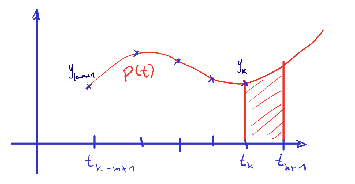
\includegraphics[width=5.96645021645022cm,height=3.08156237701692cm]{k1-10.pdf}}
\]
\begin{definition}
  \tmtextbf{(Adams-Bashforth-Verfahren)}
  
  \tmtextit{Zu AWP gem{\"a}{\ss} Def. 1.2 und {\"a}quidistantem Zeitgitter
  w{\"a}hlt man ein $m \in \mathbb{N}$.
  
  Seien $y_0, \ldots, y_{m - 1} \in \mathbb{R}^d$ geeignet gegeben.
  
  Setze $f_k \assign f (t_k, y_k)$ f{\"u}r $k \in \{ 0, \ldots, m - 1 \}$ und
  dazu $f_{k + 1} \assign f (t_{k + 1}, y_{k + 1})$.
  
  Dann definiere f{\"u}r $k \geq m - 1$:
  \begin{equation}
    y_{k + 1} \assign y_k + \tau \sum_{j = 1}^m \beta_j f_{k - m + j}
    \text{{\hspace{1.5em}}mit\quad} \beta_j \assign \int_0^1 \prod_{n = 1, n
    \neq j}^m \frac{m + s - n}{j - n}  \upright{d} s.
  \end{equation}}
\end{definition}

\begin{remark*}
  {\tmdummy}
  
  \begin{itemizedot}
    \item Alle $\beta_j$ sind von $\tau$ und $k$ unabh{\"a}ngig, also kann man
    die $\beta_j$ f{\"u}r gegebenes $m \in \mathbb{N}$ schon berechnen.
    
    \item Adams-Bashforth-Verfahren (AB-Verfahren) ist explizit. \ 
  \end{itemizedot}
\end{remark*}

\begin{example*}
  {\tmdummy}
  
  \begin{itemizedot}
    \item $m = 1$:
    
    Unter der Annahme, dass ein leeres Produkt $1$ liefert, gilt
    \[ \beta_1 = \int_0^1 \prod_{n = 1, n \neq 1}^1 \frac{1 + s - n}{j - n}
       \upright{d} s = \int_0^1 1 \upright{d} s = 1 \]
    und damit
    \[ y_{k + 1} = y_k + \tau f_{k - 1 + 1} = y_k + \tau f_k \]
    also erh{\"a}lt man das explizite Euler-Verfahren.
    
    \item $m = 2$:
    
    Es ist
    \[ \beta_1 = \int_0^1 \frac{2 + s - 2}{1 - 2} \upright{d} s = \frac{-
       1}{2}, \text{\qquad} \beta_2 = \int_0^1 \frac{2 + s - 1}{2 - 1}
       \upright{d} s = = \frac{3}{2} \]
    und somit
    \[ y_{k + 1} = y_k + \tau \left( \frac{3}{2} f_k - \frac{1}{2} f_{k - 1}
       \right) . \]
    \item $m = 4$:
    
    Es handelt sich um das ,,eigentliche Adams-Bashforth-Verfahren``, also
    \[ y_{k + 1} = y_k + \frac{\tau}{24} (55 f_k - 59 f_{k - 1} + 37 f_{k + 1}
       - 9 f_{k - 3}) . \]
  \end{itemizedot}
\end{example*}

\begin{remark*}
  \tmtextbf{(Weitere auf Integration beruhende Methoden)}
  \begin{itemizedot}
    \item Implizite Version von AB-Verfahren, also
    ``{\underline{\tmtextit{Adams-Moulton-Verfahren}}}``:
    
    Verwende eine weitere St{\"u}tzstelle, also
    \tmtextit{{\underline{einschlie{\ss}lich n{\"a}chstem Zeitpunkt}}} und
    erhalte eine Fixpunktgleichung:
    \begin{eqnarray*}
      y_{k + 1} & = & y_k + \tau \sum_{j = 1}^{m + 1} \beta_j f (t_{k - m +
      j}, y_{k - m + j})\\
      & = & y_k + \tau \sum_{j = 1}^m \beta_j f (t_{k - m + j}, y_{k - m +
      j}) + \tau \beta_{m + 1} f (t_{k + 1}, y_{k + 1})\\
      & = & y_k + \tau \sum_{j = 1}^m \beta_j \hspace{3em} f_{k - m + j}
      \hspace{2.2em} + \tau \beta_{m + 1} f (t_{k + 1}, y_{k + 1})
    \end{eqnarray*}
    mit $\{ \beta_j \}_{j = 1}^{m + 1}$ gerechnet gem{\"a}{\ss} (1.33), also
    aus $m + 1$ Punkten gerechnet.
    
    Eine M{\"o}glichkeit zur L{\"o}sung dieser Fixpunktgleichung ist das
    sogenannte
    ,,{\underline{\tmtextit{Pr{\"a}dikator-Korrektor-Verfharen}}}``, bei dem
    man das explizite AB-Verfahren zur Pr{\"a}dikation von $\hat{y}_{k + 1}$
    verwendet, und dann dies als Startwert f{\"u}r einen Korrektor-Schritt
    nimmt, d.h. 1 bis 2 Iteration eines Fixpunktverfahrens.
    
    \item Erweiterung auf Zeitpunkte {\underline{\tmtextit{vor}}} $t_k$, also
    \[ y_{k + 1} - y_{k - 1} = \int_{t_{k - 1} }^{t_{k + 1}} p (s) 
       \upright{d} s. \]
    \[ 
       \raisebox{-0.00225898963159056\height}{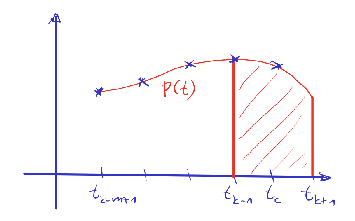
\includegraphics[width=5.96645021645022cm,height=3.71654860291224cm]{k1-11.pdf}}
    \]
    \begin{itemizeminus}
      \item Mit $p \in \mathbb{P}_{m - 1}$ Interpolation von $t \mapsto f (t,
      y (t))$ {\"u}ber $\{ t_i \}_{i = k - m + 1}^k$ ergibt
      \[ y_{k + 1} = y_{k - 1} + \tau \sum_{j = 1}^m \beta_j f_{k - m + j} \]
      und geeignete $\{ \beta_j \}_{j = 1}^m$, und das ist die
      ,,\tmtextit{{\underline{Nystrom-Methoden}}}``.
      
      \item Eine entsprechende implizite Version mit $p \in \mathbb{P}_m$
      Interpolation von $t \mapsto f (t, y (t))$ {\"u}ber $\{ t_i \}_{i = k -
      m + 1}^{k + 1}$ ist die
      ,,{\underline{\tmtextit{Milne-Simpson-Methoden}}}``.
    \end{itemizeminus}
  \end{itemizedot}
\end{remark*}

\begin{remark*}
  \tmtextbf{(Auf Differentiation beruhende Verfahren)}
  
  Die Idee dabei besteht in Polynominterpolation $q \in \mathbb{P}_m$ der
  Werte $\{ y_{k - m + j} \}_{j = 1}^{m + 1}$ mit unbekanntem Wert $y_{k +
  1}$, also
  \[ q (t) = \sum_{i = k - m + 1}^{k + 1} y_i L_i (t) \quad \text{mit\quad}
     L_i (t) = \prod_{l = k - m + 1, l \neq i}^{k + 1} \frac{t - t_l}{t_i -
     t_l} \]
  und somit gilt analog wie bei AB-Verfahren
  \[ q (t_k + s \tau) = \sum_{i = k - m + 1}^{k + 1} y_i  \prod_{l = k - m +
     1, l \neq i}^{k + 1} \frac{k + s - l}{i - l} = \sum_{j = 1}^{m + 1} y_{k
     - m + j} \prod_{n = 1, n \neq j}^{m + 1} \frac{m + n + s}{j - n} . \]
  {\hspace{1.7em}}Bei der Bedingung an dem unbekannten $y_{k + 1}$ gibt es
  zwei M{\"o}glichkeiten
  \begin{enumeratealpha}
    \item Bestimme $y_{k + 1}$ s.d. $q' (t_k) = f (t_k, y_k)$, d.h. $q'$
    erf{\"u}llt die DGL in $t_k$, also
    \begin{equation}
      q' (t_k) = \frac{1}{\tau} \frac{\partial}{\partial s} q (t_k + s \tau) |
      \nobracket_{s = 0} = \frac{1}{\tau} \sum_{j = 1}^{m + 1} y_{k - m + j}
      \left. \left( \frac{\partial}{\partial s} \prod_{n = 1, n \neq j}^{m +
      1} \frac{m - n + s}{j - n} \right) \right|_{s = 0} .
    \end{equation}
    {\hspace{1.7em}}Der Term $\alpha_j \assign \left. \left(
    \frac{\partial}{\partial s} \prod_{n = 1, n \neq j}^{m + 1} \frac{m - n +
    s}{j - n} \right) \right|_{s = 0}$ l{\"a}sst sich unabh{\"a}ngig von den
    $y_k$ im Voraus berechnen.
    
    Das Verfahren hat also die Gestalt
    \[ \sum_{j = 1}^{m + 1} \alpha_j y_{k - m + j} = \tau f (t_k, y_k) \]
    und falls $\alpha_{m + 1} \neq 0$, ist dies explizit nach $y_{k + 1}$
    aufl{\"o}sbar.
    
    \item Bestimme $y_{k + 1}$ s.d. $q' (t_{k + 1}) = f (t_{k + 1}, y_{k +
    1})$, d.h. $q'$ erf{\"u}llt die DGL in $t_{k + 1}$, also ergibt sich ein
    Verfahren der Gestalt
    \[ \sum_{j = 1}^{m + 1} \tilde{\alpha}_j y_{k - m + j} = \tau f (t_{k +
       1}, y_{k + 1}) \]
    mit $\tilde{\alpha}_j \assign \left. \left( \frac{\partial}{\partial s}
    \prod_{n = 1, n \neq j}^{m + 1} \frac{m - n + s}{j - n} \right) \right|_{s
    = 1}$.
    
    Diese Variante nennt man ,,{\underline{\tmtextit{Backward Difference
    Formulae}}}``, oder auch ,,\tmtextit{{\underline{BDF-Formeln}}}``.
  \end{enumeratealpha}
\end{remark*}

\begin{remark*}
  {\tmdummy}
  
  \begin{itemizedot}
    \item Im Prinzip kann man MSV beliebiger Ordnung definieren.
    
    \item Die Anlaufwerte (Startwerte) $y_1$, {\textdots}, $y_{m - 1}$ kann
    man mit einem ESV bestimmen, dessen Ordnung sinnvollerweise mindestens der
    Ordnung des MSV entsprechen sollte.
    
    \item Ein {\underline{\tmtextit{Vorteil von MSV}}} gegen{\"u}ber ESV
    besteht darin, dass man \tmtextit{{\underline{bei MSV nur eine
    $f$-Auswertung pro Iteration}}}. Dies ist insbesondere vorteilhaft, wenn
    die Auswertungen von $f$ teuer sind.
  \end{itemizedot}
\end{remark*}

\

\section{Randwertprobleme f{\"u}r ODEs}

Wir geben einen sehr knappen Einblick in Randwertprobleme (RWP) f{\"u}r
lineare ODEs ohne (ausf{\"u}hrliche) Beweise.

\begin{definition}
  \tmtextbf{(Inhomogenes lineares RWP)}
  
  \tmtextit{Sei $I = [a, b]$, $B_a$, $B_b \in \mathbb{R}^{d \times d}$, $A : I
  \rightarrow \mathbb{R}^{d \times d}$, $f \in C (I, \mathbb{R}^d)$, sowie $g
  \in \mathbb{R}^d$.
  
  Gesucht ist eine Funktion $y : I \rightarrow \mathbb{R}^d$ als L{\"o}sung
  von
  \begin{equation}
    \text{{\hspace{3em}}} \forall t \in I : \text{\quad} y' (t) - A (t) y (t)
    = f (t),
  \end{equation}
  \[ B_a y (a) + B_b y (b) = g. \]
  {\hspace{1.7em}}Die Gleichung (1.35) hei{\ss}t ein {\underline{Inhomogenes
  lineares RWP mit Randbedingung (RB)}} $B_a y (a) + B_b y (b) = g$. \ }
\end{definition}

Beachte: F{\"u}r $B_a = I$, $B_b = 0$ erhalten wir wieder ein lineares AWP.

\begin{definition}
  \tmtextbf{(Sturm-Liouville-Probleme)}
  
  \tmtextit{Sei $I = [a, b]$, $p \in C^1 (I, \mathbb{R}_{> 0})$, $q$, $r$, $f
  \in C (I, \mathbb{R})$, sowie $\alpha_0$, $\alpha_1$, $\beta_0$, $\beta_1$,
  $g_a$, $g_b \in \mathbb{R}$.
  
  Gesucht ist eine Funktion $y : I \rightarrow \mathbb{R}$ s.d. es gilt }
  \begin{equation}
    \text{{\hspace{3em}}} \forall t \in I : \text{\quad} - (p (t) y' (t))' + q
    (t) y' (t) + r (t) y (t) = f (t),
  \end{equation}
  \[ \alpha_1 y' (a) + \alpha_0 y (a) = g_a, \text{\quad} \beta_1 y' (b) +
     \beta_0 y (b) = g_b . \]
\end{definition}

\begin{remark*}
  {\tmdummy}
  
  \begin{itemizedot}
    \item Im Fall $q = 0$, $p = 1$, $r = 0$ und $x \assign t$ erhalten wir die
    {\underline{\tmtextit{Diffusionsgleichung}}}
    \[ \forall x \in [a, b] : \text{\quad} - y'' (x) = f (x), \]
    die beschreibt, wie sich Stoffkonzentration $y$ mit Quellterm $f$ im
    ruhenden Medium {\"o}rtlich ausbreitet, z.B. Tinte in Wasser, W{\"a}rme in
    Stab, etc.
    
    \item Die Funktion $p$ hei{\ss}t {\underline{\tmtextit{Diffusionsterm}}},
    $q$ {\underline{\tmtextit{Transportterm}}} oder
    {\underline{\tmtextit{Konvektionsterm}}}, $r$
    {\underline{\tmtextit{Reaktionsterm}}} und $f$
    {\underline{\tmtextit{Quellterm}}}. Eine allgemeine Bezeichnung f{\"u}r
    (1.36) lautet
    {\underline{\tmtextit{Konvektions-Reaktions-Diffusions-Gleichung}}}.
    
    \item Im Fall $\alpha_1 = \beta_1 = 0$ und $\alpha_0 \neq 0 \neq \beta_0$
    spricht man von der {\underline{\tmtextit{Dirichlet-Randbedingung}}}. Im
    Zusammenhang zur station{\"a}ren W{\"a}rmeleitung (vgl. Anfang des
    Kapitels) gibt die Dirichlet-Randbedingung die Temperaturen an Randpunkte
    vor.
    
    \item Im Fall $\alpha_0 = \beta_0 = 0$ und $\alpha_1 \neq 0 \neq \beta_1$
    spricht man von der {\underline{\tmtextit{Neumann-Randbedingung}}},
    insbesondere spricht man bei $y' (a) = 0 = y' (b)$ von
    {\underline{\tmtextit{isolierender Randbedingung}}}.
    
    \item {\underline{\tmtextit{SL-Problem ist ein Spezialfall vom
    inhomogenen linearen RWP}}}.
    
    Dies sieht man, wenn man das SL-Problem als System erster Ordnung
    schreibt:
    
    $y$ l{\"o}st (1.36), d.h.
    \[ - p' y' - p y'' + q y' + r y = f \text{\quad mit RB\quad}
       \left\{\begin{array}{l}
         \alpha_1 y' (a) + \alpha_0 y (a) = g_a\\
         \beta_1 y' (b) + \beta_0 y (b) = g_b
       \end{array}\right. \]
    \[ \Leftrightarrow \]
    $\left(\begin{array}{c}
      z_1\\
      z_2
    \end{array}\right) \assign \left(\begin{array}{c}
      y\\
      y'
    \end{array}\right)$ l{\"o}st
    \[ \left(\begin{array}{c}
         z_1'\\
         z_2'
       \end{array}\right) - \left(\begin{array}{cc}
         0 & 1\\
         \frac{r}{p} & \frac{q - p'}{p}
       \end{array}\right) \left(\begin{array}{c}
         z_1\\
         z_2
       \end{array}\right) = \left(\begin{array}{c}
         0\\
         - \frac{f}{p}
       \end{array}\right) \]
    \[ \text{\quad mit RB\quad} \left(\begin{array}{cc}
         \alpha_0 & \alpha_1\\
         0 & 0
       \end{array}\right) \left(\begin{array}{c}
         z_1 (a)\\
         z_2 (a)
       \end{array}\right) + \left(\begin{array}{cc}
         0 & 0\\
         \beta_0 & \beta_1
       \end{array}\right) \left(\begin{array}{c}
         z_1 (b)\\
         z_2 (b)
       \end{array}\right) = \left(\begin{array}{c}
         g (a)\\
         g (b)
       \end{array}\right), \]
    also ist $B_a \assign \left(\begin{array}{cc}
      \alpha_0 & \alpha_1\\
      0 & 0
    \end{array}\right)$, $B_b \assign \left(\begin{array}{cc}
      0 & 0\\
      \beta_0 & \beta_1
    \end{array}\right)$ und $g \assign \left(\begin{array}{c}
      g (a)\\
      g (b)
    \end{array}\right)$.
  \end{itemizedot}
\end{remark*}

Es stellt sich nat{\"u}rlich die Frage, ob die L{\"o}sungen zu inh. lin. RWP
bzw. zu SL-Problemen existieren oder im Fall Existenz eindeutig sind.

Wir kl{\"a}ren zun{\"a}chst die Eindeutigkeit von L{\"o}sung zu SL-Problem,
denn die Sturktur des Beweises wird sp{\"a}ter oft auftauchen.

\begin{theorem}
  \tmtextbf{(Eindeutigkeit von L{\"o}sung eines SL-Problems) }
  
  \tmtextit{Das SL-Problem gem{\"a}{\ss} Def. 1.40 mit Dirichlet-Randbedingung
  ($\alpha_1 = \beta_1 = 0$ und $\alpha_0 \neq 0 \neq \beta_0$) hat
  h{\"o}chstens eine L{\"o}sung $y \in C^2 ((a, b), \mathbb{R}) \cap C ([a,
  b], \mathbb{R})$, falls die folgenden drei Bedingungen erf{\"u}llt sind:
  \begin{itemizedot}
    \item $p$ ist ,,echt-positiv``, d.h. \ $\exists p_0 \in \mathbb{R} \forall
    t \in [a, b] : \text{\enspace} p (t) \geq p_0 > 0$,
    
    \item $p, q \in C^1$
    
    \item Die Daten erf{\"u}llen noch eine Ungleichung
    \[ p_0 + (b - a)^2 \min_{t \in [a, b]} \left( r (t) - \frac{1}{2} q' (t)
       \right) > 0. \]
  \end{itemizedot}}
\end{theorem}

\begin{proof}
  Es reicht zu zeigen, dass das zugeh{\"o}rige homogene Problem ($f = 0$, $g_a
  = g_b = 0$) nur triviale L{\"o}sung hat, d.h. sei $y$ eine L{\"o}sung von
  \begin{equation}
    - (p y')' + q y' + r y = 0
  \end{equation}
  mit $y (a) = y (b) = 0$, und wir zeigen $y = 0$.
  
  (Um Notation zu vereinfachren, schreiben wir bei Integranten $p$ statt $p
  (t)$, sofern es im Kontext klar ist.)
  \begin{enumerateroman}
    \item {\underline{Multiplizieren (1.37) mit $y$ und Integrieren {\"u}ber
    $[a, b]$}} ergibt
    \[ - \int_a^b (p y')' y \upright{d} t + \int_a^b q y' y \upright{d} t +
       \int_a^b r y^2 \upright{d} t = 0. \]
    {\hspace{1.7em}}{\underline{Partielle Integration}} beim 1. \& 2. Term
    liefert
    \begin{eqnarray*}
      - \int_a^b (p y')' y \upright{d} t & = & \int_a^b p y' y' \upright{d} t
      - [p y' y] | \nobracket_a^b\\
      \int_a^b q y' y \upright{d} t & = & - \int_a^b \frac{1}{2} q' y^2
      \upright{d} t + \left. \left[ \frac{1}{2} q y^2 \right] \right|_a^b
    \end{eqnarray*}
    wobei die beiden Auswertungsterme $0$ sind, da $y (a) = y (b) = 0$.
    
    Wir fassen die drei {\"u}brigen Integralterme zusammen und erhalten
    \[ \int_a^b p (y')^2 \upright{d} t + \int_a^b \left( r - \frac{1}{2} q'
       \right) y^2 \upright{d} t = 0. \]
    \item Absch{\"a}tzen der linken Seite nach Unten liefert
    \begin{eqnarray*}
      0 & = & \int_a^b p (y')^2 \upright{d} t + \int_a^b \left( r -
      \frac{1}{2} q' \right) y^2 \upright{d} t\\
      & \geq & \int_a^b p (y')^2 \upright{d} t + \min_{t \in [a, b]} \left( r
      - \frac{1}{2} q' \right) \int_a^b y^2 \upright{d} t\\
      & \geq & p_0 \int_a^b (y')^2 \upright{d} t + \min_{t \in [a, b]} \left(
      r - \frac{1}{2} q' \right) \int_a^b y^2 \upright{d} t
    \end{eqnarray*}
    wobei die 3. Zeile die ,,echte Positivit{\"a}t`` von $p$ genutzt hat.
    
    Also wir erhalten
    \begin{equation}
      p_0 \int_a^b (y')^2 \upright{d} t + \min_{t \in [a, b]} \left( r -
      \frac{1}{2} q' \right) \int_a^b y^2 \upright{d} t \leq 0.
    \end{equation}
    
    
    \item Hilfswerkzeug: ($1$ dimensionale) Poincar{\'e}-Ungleichung
    \[ \forall u \in C^1 ([a, b], \mathbb{R})  \text{mit } u (a) = 0 :
       \text{\qquad} \int_a^b u^2 \upright{d} t \leq (b - a)^2 \int_a^b (u')^2
       \upright{d} t. \]
    Beweis dazu:
    
    Es ist
    \begin{eqnarray*}
      u {(t)^2}  & = & \left( u (a) + \int_a^t u^{'} (s) \upright{d} s
      \right)^2\\
      & = & \left( \text{\quad} 0 \enspace + \int_a^t 1 \cdot u^{'} (s)
      \upright{d} s \right)^2\\
      & \leq & \left( \left( \int_a^t 1^2 \upright{d} s \right)^{\frac{1}{2}}
      \cdot \left( \int_a^t (u^{'})^2 \upright{d} s \right)^{\frac{1}{2}}
      \right)^2\\
      & = & \text{\qquad} \int_a^t 1  \upright{d} s \quad \cdot \text{\qquad}
      \int_a^t (u^{'})^2 \upright{d} s\\
      & \leq & \text{\qquad} \int_a^b 1  \upright{d} s \quad \cdot
      \text{\qquad} \int_a^b (u^{'})^2 \upright{d} s\\
      & = & \text{\qquad} (b - a) \quad \cdot \text{\qquad} \int_a^b
      (u^{'})^2 \upright{d} s
    \end{eqnarray*}
    wobei die 3. Zeile aus Cauchy-Schwarz-Ungleichung folgt, und somit gilt
    \[ \text{\qquad} \int_a^b u^2 \upright{d} t \leq (b - a) \max_{t \in [a,
       b]} u (t)^2 \leq (b - a)^2 \int_a^b (u^{'})^2 \upright{d} s. \]
    \item Anwendung von iii. auf $\int_a^b (y')^2 \upright{d} t$ ergibt
    \[ \int_a^b (y')^2 \upright{d} t \geq (b - a)^{- 2} \int_a^b y^2
       \upright{d} t \]
    und somit wird (1.38) zu
    \[ \left( p_0 (b - a)^{- 2} + \min_{t \in [a, b]} \left( r (t) -
       \frac{1}{2} q' (t) \right) \right) \int_a^b y^2 \upright{d} t \leq 0.
    \]
    {\hspace{1.7em}}Nach Voraussetzung ist der komplizierte Term positiv, und
    das Integral ist nicht negativ da Integrand nicht negativ, also muss
    $\int_a^b y^2 \upright{d} t = 0$ sein, und das bedeutet $y \equiv 0$.
  \end{enumerateroman}
\end{proof}

Wir bemerken hier, dass {\underline{\tmtextit{Multiplikation mit Testfunktion
und partielle Integration werden wesentliche Zutate f{\"u}r Finite Elemente}}}
im Kapitel 3 sein.

Die Existenzaussagen f{\"u}r SL-Probleme betrachten wir nicht separat,
sondern wir untersuchen jetzt die Existenz- und Eindeutigkeitsaussage f{\"u}r
allgemeine inhomogenen lineare RWP:

\begin{remark*}
  \tmtextbf{(Existenz \& Eindeutigkeit f{\"u}r allgemeine lineare RWP)}
  
  Sei ein inhomogenes lineares RWP gem{\"a}{\ss} Def. 1.39 gegeben, d.h.
  gesucht ist eine L{\"o}sung $y : I \rightarrow \mathbb{R}^d$ s.d.
  \[ \text{{\hspace{3em}}} \forall t \in I : \text{\quad} y' (t) - A (t) y
     (t) = f (t) \text{\quad} \wedge \text{\quad} B_a y (a) + B_b y (b) = g \]
  mit $I = [a, b]$, $B_a$, $B_b \in \mathbb{R}^{d \times d}$, $A : I
  \rightarrow \mathbb{R}^{d \times d}$, $f \in C (I, \mathbb{R}^d)$, sowie $g
  \in \mathbb{R}^d$.
  \begin{enumerate}
    \item Betrachte hierzu $d + 1$ AWP f{\"u}r Funktionen $u_0$, {\textdots},
    $u_d : I \rightarrow \mathbb{R}^d$
    \begin{equation}
      \begin{array}{lll}
        & u'_0 (t) - A (t) u_0 (t) = f (t), & u_0 (a) = 0\\
        & u'_i (t) - A (t) u_i (t) = 0, & u_i (a) = e_i
      \end{array}
    \end{equation}
    mit $i \in \{ 1, \ldots, d \}$ und $\{ e_i \}_{i = 1}^d$ den
    Einheitsvektoren.
    
    \item Jedes AWP in (1.39) ist eindeutig l{\"o}sbar nach
    Picard-Lindel{\"o}f und wir bilden mit den $d$ L{\"o}sungen $u_1$,
    {\textdots}, $u_d$ die Fundamentalmatrix
    \[ U (t) \assign \left(\begin{array}{ccc}
         u_1 (t) & \cdots & u_d (t)
       \end{array}\right) \in \mathbb{R}^{d \times d} . \]
    \item Die L{\"o}sungen zu $y' (t) - A (t) y (t) = f (t)$ bildet nach
    Analysis 3 bilden einen $d$-dimensionalen affinen L{\"o}sungsraum.
    
    Elemente davon sind genau in der Form
    \begin{equation}
      y (t) = u_0 (t) + \sum_{i = 1}^d s_i u_i (t) = : u_0 (t) + U (t) \cdot s
    \end{equation}
    mit Koeffizientenvektor $s \assign (s_i)_{i = 1}^d \in \mathbb{R}^d$, denn
    diese l{\"o}sen die DGL
    \begin{eqnarray*}
      y' (t) & = & \text{{\hspace{2.5em}}} u_0' (t) \hspace{2.5em} +
      \text{\quad} U' (t) s\\
      & = & f (t) + A (t) u_0 (t) + A (t) U (t) s\\
      & = & f (t) + A (t) (u_0 (t) + U (t) s)\\
      & = & f (t) + A (t) y (t) .
    \end{eqnarray*}
    \item Die Randbedingungen liefert Gleichung f{\"u}r $s$:
    \begin{eqnarray*}
      &  & B_a y (a) + B_b y (b) = g\\
      & \Leftrightarrow & B_a u_0 (a) + B_a U (a) s + B_b u_0 (b) + B_b U (b)
      s = g\\
      & \Leftrightarrow & B_a \quad 0 \quad + B_a \hspace{0.8em} I
      \hspace{0.8em} s + B_b u_0 (b) + B_b U (b) s = g\\
      & \Leftrightarrow & (B_a + B_b U (b)) s = g - B_b u_0 (b) .
    \end{eqnarray*}
    Falls $B_a + B_b U (b)$ invertierbar ist, dann erhalten wir
    \[ s = (B_a + B_b U (b))^{- 1} (g - B_b u_0 (b)) . \]
  \end{enumerate}
\end{remark*}

Das obige Ergebnis fassen wir in einem Satz zusammen:

\begin{theorem}
  \tmtextbf{(Existenz \& Eindeutigkeit von L{\"o}sung zu inh. lin. RWP)}
  
  \tmtextit{Ein inhomogenes lineares RWP gem{\"a}{\ss} Def. 1.39 besitzt eine
  eindeutige L{\"o}sung, g.d.w. die Matrix
  \[ Q \assign B_a + B_b U (b) \]
  invertierbar ist. }
\end{theorem}

Unsere {\"U}berlegungen von vorhin sind zwar konstruktiv, aber nicht numerisch
durchf{\"u}hrbar.

Um dies nachzuholen, f{\"u}hren wir die
{\underline{\tmtextit{Schie{\ss}verfahren}}} ein:

\begin{definition}
  \tmtextbf{(Einfach-Schie{\ss}verfahren)}
  
  \tmtextit{Sei ein allgemeines inhomogenes lineares RWP gem{\"a}{\ss} Def.
  1.39 gegeben.
  
  W{\"a}hle ein Gitter $\Delta$ auf $I = [a, b]$.
  
  F{\"u}r $j \in \{ 0, \ldots, d \}$ berechne mit ESV oder MSV approximative
  L{\"o}sung \ }
  \[ \forall k \in \{ 0, \ldots, K \} : \text{\quad} u_{j, k} \approx u_j
     (t_k) \]
  zu den $d + 1$ AWP in (1.39).
  
  Definiere die {\underline{\tmtextit{diskrete Fundamentalmatrix}}} zur
  Endzeit
  \[ U_{\tau} \assign \left(\begin{array}{ccc}
       u_{1, K} & \cdots & u_{d, K}
     \end{array}\right) \in \mathbb{R}^{d \times d} \]
  und damit die diskrete Schie{\ss}matrix
  \[ Q_{\tau} \assign B_a + B_b U_{\tau} . \]
  {\hspace{1.7em}}Falls $Q_{\tau}$ invertierbar ist, l{\"o}se das LGS nach
  $s_{\tau} \assign (s_{\tau, j})_{j = 1}^d \in \mathbb{R}^d$, also l{\"o}se
  \[ Q_{\tau} s_{\tau} = g - B_b u_{0, K} \]
  und erhalte eine approximative L{\"o}sung des RWP
  \[ \forall k \in \{ 0, \ldots, K \} : \text{\quad} y_k \assign u_{0, k} +
     \sum_{j = 1}^d s_{\tau, j} u_{j, k} . \]
\end{definition}

\begin{theorem}
  \tmtextbf{(Konvergenz vom Schie{\ss}verfahren)}
  
  \tmtextit{Falls RWP wohldefiniert ist, d.h. $Q$ invertierbar, so ist f{\"u}r
  gen{\"u}gend kleine $\tau \leq \tau_{\max}$ die diskrete Schie{\ss}matrix
  $Q_{\tau}$ invertierbar.
  
  Falls ESV / MSV f{\"u}r $\{ u_i \}_{i = 0}^d$ besitzt Ordnung $p$ nach Satz
  1.18, dann konvergiert das Einfach-Schie{\ss}verfahren mit Ordnung $p$. }
\end{theorem}

\begin{proof}
  (Skizze)
  
  Beim ESV haben wir gesehen, dass es f{\"u}r geeignete $C$, $\tilde{C} \in
  \mathbb{R}$ gilt
  \begin{equation}
    \| u_{j, k} - u_j (t_k) \| \leq C\mathbf{e}^{\tilde{C} (t_k - a)} \tau^p .
  \end{equation}
  {\hspace{1.7em}}Damit zeigt man, dass $\| U_{\tau} - U (t_k) \|$ und $\| Q -
  Q_{\tau} \|$ klein sind.
  
  Dann folgt mit LGS-Stabilit{\"a}t, dass $\| s - s_{\tau} \|$ ebenfalls
  klein ist und mit Stetigkeit von Norm auch $\| y_k - y (t_k) \|$ mit Ordnung
  $p$ konvergiert. 
\end{proof}

Wir bemerken hier, dass der Begriff ,,Schie{\ss}verfahren`` auf ballistischen
Anwendungen beruht.

\begin{remark*}
  \tmtextbf{(Erweiterungen)}
  \begin{itemizedot}
    \item {\underline{\tmtextit{Mehrfach-Schie{\ss}verfahren}}}
    
    Fehler in (1.41) k{\"o}nnte durch gro{\ss}e Intervalle $I$ ggf. sehr
    gro{\ss} sein.
    
    Idee: Intervalle $I$ wird in $M$ grobe Intervalle zerlegt und das RWP in
    Form von $M$ gekoppelten RWP formuliert.
    
    Dies f{\"u}hrt auf ein LGS f{\"u}r Koeffizienten $s_m \in \mathbb{R}^d$
    auf Teilintervallen mit $m \in \{ 1, \ldots, M \}$.
    
    Dieses LGS ist gr{\"o}{\ss}er als bei Einfach-Schie{\ss}verfahren, aber
    bessere Genauigkeit wird damit erreichbar.
    
    \item {\underline{\tmtextit{Nichtlineare RWP}}}
    
    Suche $y : I \rightarrow \mathbb{R}^d$ s.d.
    \[ \forall t \in I : \text{\qquad} y' (t) = f (t, y (t)) \quad \wedge
       \text{\quad} r (y (a), y (b)) = 0. \]
    {\hspace{1.7em}}Ansatz: Formuliere ein parametrisches AWP bzgl. ein $s \in
    \mathbb{R}^d$, also
    \[ \forall t \in I : \text{\qquad} y' (t, s) = f (t, y (t, s)) \quad
       \wedge \text{\quad} y (a, s) = s. \]
    und bestimme $s$ der Art, s.d. $F (s) \assign r (y (a, s), y (b, s)) = 0$
    wird.
    
    Also entsteht dadurch ein Nullstellenproblem f{\"u}r $F (s)$.
    
    Dies kann man z.B. mit
    \tmtextit{{\underline{Fixpunkt-Schie{\ss}verfahren}}} l{\"o}sen, d.h.
    w{\"a}hle geeignetes $s^{(0)} \in \mathbb{R}^d$ und setze
    \[ s^{(m + 1)} \assign s^{(m)} - C F (s^{(m)}) \]
    mit einer invertierbaren Matrix $C$.
    
    Dabei sind die Iterationen teuer, weil Auswertung von $F$ L{\"o}sung
    eines AWP erfordert, um $y (b, s)$ zu bestimmen.
    
    Speziell mit $C \assign D F$ erhalten wir das
    {\underline{\tmtextit{Newton-Schie{\ss}verfahren}}}. 
  \end{itemizedot}
\end{remark*}

\end{document}
